% ><><><><><><><><><><><><><><><><><><><><><><><><><><><><><><><><><><><><><><
%       Mines LaTeX Thesis Template. 
% ><><><><><><><><><><><><><><><><><><><><><><><><><><><><><><><><><><><><><><
% This template was written for pdfLaTex Compilers
\documentclass[letterpaper,10pt]{article} %% <-- INPUT: Font size below, change the number to 10, 11 or 12pt

% ------------------------------------------------- Packages & Setup
\usepackage{csm-thesis}         % Proper Thesis Formatting. This requires the 'csm-style-files' directory

\usepackage{array}              % For inserting large multi-page tables
\usepackage{longtable}

\usepackage[numbers]{natbib}    % For proper citations
\usepackage{hyperref}           % For referencing though out the document. Can change, look at user manual how to change
\usepackage{pdflscape}          % For inserting landscape-mode objects 
\usepackage{amsmath}            % For matrices

% ----- Needed by the journal chapters (quantum circuits, schematics, tables) -----
\usepackage{xcolor}             % Colors for the figures drawn in TeX
\usepackage{tikz}               % Schematic diagrams (graphicx is loaded by csm-thesis)
\usetikzlibrary{arrows.meta, fit, backgrounds, shapes.geometric, positioning, calc}
\usepackage{quantikz}           % Quantum circuit diagrams
\makeatletter\@ifundefined{ket}{\usepackage{braket}}{}\makeatother % \ket, if quantikz does not provide it
\usepackage{booktabs}           % \toprule, \midrule, \bottomrule

% ----- REVTeX/quantumarticle constructs from the Chapter 3 paper -----
% The thesis is single-column, so these two-column helpers are no-ops here.
% widetext widened content across a two-column page; here it shrinks it to fit
\newenvironment{widetext}{\small}{}
\providecommand{\onecolumngrid}{}
\providecommand{\twocolumngrid}{}
\providecommand{\squeezetable}{}

% ----- Notation and environments used by the journal chapters -----
\newtheorem{lemma}{Lemma}[section]      % "Lemma 3.1" (chapters are sections here)
\newenvironment{lemproof}{\par\noindent\emph{Proof.}\ }{\hfill$\blacksquare$\par\medskip}
\newcommand{\diag}{\operatorname{diag}}
\newcommand{\lamax}{\lambda_{\max}}
\newcommand{\Ht}{\widetilde{H}_1}
\newcommand{\At}{\widetilde{A}}
% NOTE: do not use \makecell (or any nested tabular) inside a table float; the
% template rejects it with "Caption must be above table". Use \shortstack instead.
% --------------------------------------------------------------------------------
\usepackage{listings}           % For inserting programming code
\usepackage{rotating}           % For inserting sideways tables and figures
\usepackage{lipsum}             % For dummy text. You can remove this once you have remove all of the example text. 

\usepackage{my-Equations}       % Where I define frequently used equations or symbols for easy use

% For using row-spanning and column-spanning in tables:
%\usepackage{multirow}


% For using helvetica instead of Computer Modern
% \usepackage{helvet}
% \renewcommand{\familydefault}{\sfdefault}
% ~~~~~~~~~~~~~~~~~~~~~~~~~~~~~~~~~~~~~~~~~~~~~~~~~~~~~ Place To Look For Figures
% This tells the pdf builder where to look for the figures that are added in the document
% you can add more paths if you wish, example:
% \graphicspath{{./figures/}{./figures/try-me}}
\graphicspath{{./figures/}}

% ><><><><><><><><><><><><><><><><><><><><><><><><><><><><><><><><><><><><><
%       GENERAL USER INFO: Title, Authors, Advisors...
% ><><><><><><><><><><><><><><><><><><><><><><><><><><><><><><><><><><><><><
% ~~~~~~~~~~~~~~~~~~~~~~~~~~~~~~~~~~~~~~~~~~~~~~~~~~~~~  TITLE
\title{
    Quantum Computing for Partial Differential\\%
    Equations and Inverse Problems
    }

% ~~~~~~~~~~~~~~~~~~~~~~~~~~~~~~~~~~~~~~~~~~~~~~~~~~~~~ PERSONAL INFORMATION
\degreetitle{Doctor of Philosophy} % Degree Title like Master of Science or Doctor of Philosophy
\discipline{Geophysics}             % Area of research, eg. Applied Physics
\department{School of Earth, Space and Planets} % Full unit name as printed, eg. Department of Physics

\author{Hoang Anh Nguyen}        % your NAME, don't forget your middle names.
\advisor{Dr. Ge Jin}                % your Advisor, put Dr. in front if they have a PhD them selves!
\coadvisor{Dr. Ali Tura}            % if you have a co-advisor, otherwise Comment out/remove the line
\dpthead{Dr. Big Boss}{Department Head Title}    % department head name & title. eg. \dpthead{Dr. Uwe Greife}{Professor and Department Head}

\begin{document}
% ><><><><><><><><><><><><><><><><><><><><><><><><><><><><><><><><><><><><><
%       FRONT MATTER
% ><><><><><><><><><><><><><><><><><><><><><><><><><><><><><><><><><><><><><
% If you do not want any of the following 'optional' items, either comment 
%   out those lines, or remove them from the document. Or if you do not have
%   any Figures, Tables, Symbols, or Abbreviations you can remove those lists.

\frontmatter                       % Leave this line here, it sets the formatting 
                                   % requirements for the front matter of the document
\maketitle\newpage                 % >>>>>>>>> Title Page (required) <<<<<<<<<
\makecopyright{\the\year}\newpage  % >>>>>>>>> Copyright Page (optional) <<<<<<<<< 
\makesubmittal\newpage             % >>>>>>>>> Signature Page (required) <<<<<<<<<

% >>>>>>>>>>>>>>>>>>>>>>>>>>>>> Abstract (required) <<<<<<<<<<<<<<<<<<<<<<<<<<<<<
\begin{abstract}
\input{chapter/i-abstract}
% you can also directly type your abstract here if you prefer.
\end{abstract} \newpage

% >>>>>>>>>>>>>>>>>>>>>>>>>>>>>>>>>>>>>>> <<<<<<<<<<<<<<<<<<<<<<<<<<<<<<<<<<<<<<<

\tableofcontents\newpage        % >>>>>>>>> Table of Contents (required) <<<<<<<<<<<
\listoffigures\newpage          % >>>>>>>>> List of Figures (if applicable) <<<<<<<<
\listoftables\newpage           % >>>>>>>>> List of Tables (if applicable) <<<<<<<<<

% >>>>>>>>>>>>>>>>>>>>>>> List of Symbols (if applicable) <<<<<<<<<<<<<<<<<<<<<<<
% \ShowSymbolFirst                      % un-comment to show the symbols on the left of the list.
\listofsymbols*                         % the * puts the list in alphabetical order
\listofsymbols{General Nomenclature}    % calling a sub list
\newpage

% >>>>>>>>>>>>>>>>>>>> List of Abbreviations (if applicable) <<<<<<<<<<<<<<<<<<<<
\listofabbreviations*                  % the * puts the list in alphabetical order
\newpage

% >>>>>> Define Your Symbols and Abbreviations In the File Under 'supporting-files'
\input{supporting-files/symbols-and-abbreviations}

% >>>>>>>>>>>>>>>>>>>>>>>>>> Acknowledgments (optional) <<<<<<<<<<<<<<<<<<<<<<<<<
\begin{acknowledgments}
I would like to thank and acknowledge $<$advisor$>$ $<$family$>$ $<$funding sources$>$ $<$committee$>$.
%Write an acknowledgement that is appropriate to you and your work. You may decide who you want to include.
\end{acknowledgments} \newpage

% >>>>>>>>>> Dedication (optional) <<<<<<<<<<
% >>>>>>>>>>>>>>>>>>>>>>>>>>>>>>>>>>>>>>> <<<<<<<<<<<<<<<<<<<<<<<<<<<<<<<<<<<<<<<
% >>>>>>>>>>>>>>>>>>>>>>>>>>>>>>>>>>>>>>> <<<<<<<<<<<<<<<<<<<<<<<<<<<<<<<<<<<<<<<
\begin{dedication}
For those that shall follow after.
\addsymbol{hello}{$\cdots$}     %<-- you can add symbols and abbreviations anywhere in the text but it is good to keep them organized in one spot!
\end{dedication}\newpage


% ><><><><><><><><><><><><><><><><><><><><><><><><><><><><><><><><><><><><><><><><
%                   BODY: All Chapters and Sections
% ><><><><><><><><><><><><><><><><><><><><><><><><><><><><><><><><><><><><><><><><
\bodymatter     % Leave this line here, it sets the formatting requirements for the front matter of the document

% You can directly add you chapter text into this document. But to keep organized you
% are advised to separate you chapters into their own files, as this example shows
\chapter{Introduction}\label{chap:introduction}

% TODO: motivation, research questions, contributions, and an outline of the dissertation.
This chapter is a placeholder for the introduction.

\chapter{Background}\label{chap:background}

% TODO: PDEs and inverse problems in geophysics; fundamentals of quantum computing.
This chapter is a placeholder for the background.

\chapter{Convolution Absorbing Boundaries for Explicit-Circuit Quantum Simulation of the Wave Equation}\label{chap:qawave}

\begin{center}
    A paper submitted to \emph{Quantum}.

    Hoang Anh Nguyen\footnote{Department of Geophysics, Colorado School of Mines, Golden, Colorado 80401, USA}$^,$\footnote{Primary researcher and author for correspondence}
\end{center}

\subsection{Abstract}

Explicit quantum circuits for the wave equation via Hamiltonian simulation
[Sato \emph{et al.}, Phys.\ Rev.\ Research \textbf{6}, 033246 (2024)] are
restricted to closed (Dirichlet/Neumann/periodic) domains, in which
outgoing waves reflect back into the computational region.  We add
absorbing boundaries of the convolution type---the
complex-frequency-shifted perfectly matched layer (CPML) implemented
through exponential-kernel memory variables---and make the resulting
non-unitary dynamics quantum-implementable by Schr\"odingerisation.  We
obtain three results.  (i)~Explicit gate-level circuits for the absorbing
evolution, obtained by extending the Bell-basis term-evolution circuit of
Sato \emph{et al.}\ to projector-valued operator strings and Trotterising
to second order, demonstrated end to end on 17--21 qubits with
$10^{-3}$--$10^{-2}$ accuracy against exact references.  (ii)~A structural
obstruction: the memory-form CPML generator has an irreducibly indefinite
Hermitian part, $\lamax(H_1)=\Theta(\sqrt{\sigma_{\max}c/h})$ under any
diagonal rescaling of the memory fields, which by the recovery threshold
of Jin, Liu, and Ma costs $e^{2\lamax T}$ in post-selection.  (iii)~A
remedy: a classically precomputed Lyapunov symmetrizer renders the
transformed generator dissipative, replacing the $T$-dependent penalty by
a $T$-independent conditioning factor, measured at
$\kappa_2(S)=4.0\times10^{2}$--$8.6\times10^{2}$ at shift
$\epsilon=10^{-2}$ on grids with up to $n=4096$ unknowns, saturating under mesh refinement.  The measured
crossover times $T^{*}=\ln\kappa^{2}/(2\lambda^{+})\approx 7$--$16$ are
short: beyond them the symmetrized recovery wins by 4--26 orders of
magnitude in post-selection cost and, at the longest horizons tested, is
the only working recovery.
% ======================================================================
\subsection{Introduction}
\label{ch3:sec:intro}

Quantum algorithms for partial differential equations (PDEs) divide into
oracle-based constructions, which assume block-encoded or sparse-access
operators \cite{costa2019wave,novikau2023qsvt}, and the explicit-circuit
line initiated for hyperbolic problems by Sato \emph{et
al.}~\cite{sato2024hamiltonian}, in which every gate of the time-stepping
circuit is written down and the cost is dominated by a number of
elementary operations polynomial in the register size.  Explicit-circuit constructions for wave-type equations published to date
operate on \emph{closed} domains: Dirichlet, Neumann, or periodic
boundaries, for which the semi-discrete generator is skew-Hermitian and
the evolution is genuinely
unitary~\cite{sato2024hamiltonian,bosch2025sources}; the extension to
nonconservative systems~\cite{sato2025nonconservative} admits a bulk
damping term $\zeta(x)\,\partial_t u$ via a linear combination of
Hamiltonian simulations, but its boundaries remain closed walls and its
demonstrations are confined to the undamped acoustic and uniform heat
equations.  Scattering and radiation problems,
however, are posed on open domains; truncating the domain with hard walls
reflects every outgoing wave back into the region of interest.  Classical
solvers handle this with absorbing layers, the de facto standard being the
perfectly matched layer (PML) and its convolutional,
complex-frequency-shifted variant
(CPML)~\cite{roden2000cpml,komatitsch2007unsplit,collino2001pml,duru2022pmlreview}.
Absorption is dissipation: the generator acquires a non-trivial Hermitian
part, and the dynamics ceases to be unitary.

Schr\"odingerisation~\cite{jin2023schrodingerisation} is a general route
for running such non-unitary linear dynamics on a quantum computer: the
warped phase-space transform turns $\dot z = Az$ into a genuine
Hamiltonian evolution on one extra register, at the price of a
post-selected recovery slice.  \ref{ch3:fig:pipeline} summarises the
resulting four-step structure of this work.

\begin{figure}[tb]
  \centering
  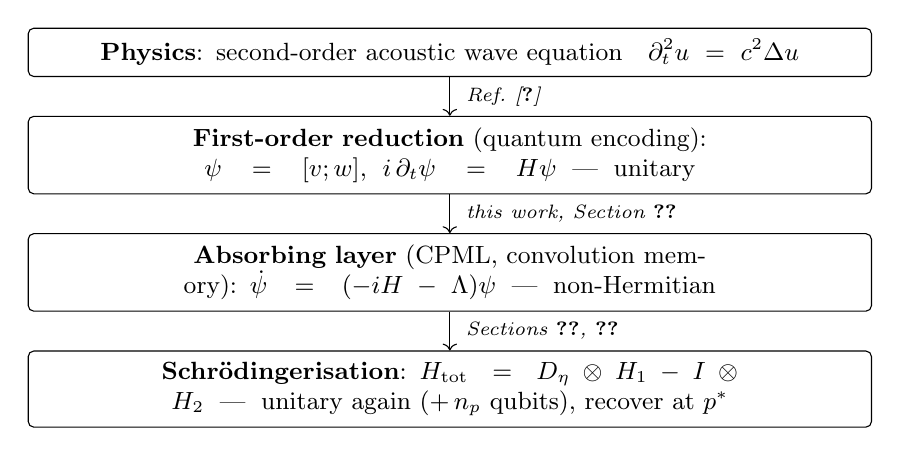
\begin{tikzpicture}[
      box/.style={draw, rounded corners=2pt, align=center,
                  inner sep=4pt, font=\small, text width=0.86\linewidth},
      lab/.style={font=\scriptsize\itshape, anchor=west},
      node distance=14pt]
    \node[box] (b1) {\textbf{Physics}: second-order acoustic wave
      equation\quad $\partial_t^2 u = c^2\Delta u$};
    \node[box, below=of b1] (b2) {\textbf{First-order reduction}
      (quantum encoding): $\psi=[v;w]$,\;
      $i\,\partial_t\psi = H\psi$ \;---\; unitary};
    \node[box, below=of b2] (b3) {\textbf{Absorbing layer} (CPML,
      convolution memory): $\dot\psi = (-iH-\Lambda)\psi$ \;---\;
      non-Hermitian};
    \node[box, below=of b3] (b4) {\textbf{Schr\"odingerisation}:
      $H_{\mathrm{tot}} = D_\eta\otimes H_1 - I\otimes H_2$ \;---\;
      unitary again ($+\,n_p$ qubits), recover at $p^{*}$};
    \draw[->] (b1) -- node[lab] {\;Ref.~\cite{sato2024hamiltonian}} (b2);
    \draw[->] (b2) -- node[lab] {\;this work, Section~\ref{ch3:sec:generators}} (b3);
    \draw[->] (b3) -- node[lab] {\;Sections~\ref{ch3:sec:schro},
      \ref{ch3:sec:circuits}} (b4);
  \end{tikzpicture}
  \caption{The four-step structure: second-order acoustic physics,
  first-order quantum encoding, convolution absorbing layer applied in
  that first-order form, and Schr\"odingerisation restoring unitarity.
  The cost of step three---the indefiniteness quantified by
  Lemma~\protect\ref{ch3:lem:threshold}---and its remedy (the Lyapunov symmetrizer)
  are the subject of Section~\protect\ref{ch3:sec:symmetrizer}.}
  \label{ch3:fig:pipeline}
\end{figure}  The programme now spans artificial boundary
conditions for the time-dependent Schr\"odinger
equation~\cite{jin2024abc}, inhomogeneous terms and the recovery-threshold
theory~\cite{jin2024recovery}, ill-posed problems~\cite{jin2024illposed},
Maxwell's equations~\cite{jin2023maxwell,ma2024maxwellcircuits}, elastic
waves~\cite{jin2025elastic}, gate-level circuits for parabolic
problems~\cite{hu2024quantum,jin2024heat}, query-optimal
formulations~\cite{jin2025queries}, and implicit-explicit integrators
for multiscale dynamics including the bulk-damped telegraph
equation~\cite{hu2026imex}.  What it does not yet contain is an
absorbing boundary for a classical wave-type equation, at either matrix or
circuit level.

\subsubsection{Related work and positioning}
\label{ch3:sec:related}

The positioning below was verified by a full-text literature review
through June 2026.\footnote{Adversarially cross-checked sweep over
published and preprinted work, 2023--2026; all primary claims below were
confirmed against the full texts of the cited papers.}

\noindent\textbf{The core niche is open.}  No published or preprinted work
through June 2026 combines any absorbing boundary (PML, CPML, complex
absorbing potential, sponge, or Dirichlet-to-Neumann map) for
\emph{classical wave-type equations} with Schr\"odingerisation or any
other unitarisation, at matrix or circuit level.  Jin and
Zhang~\cite{jin2025elastic} (elastic waves) state verbatim that
non-periodic boundaries ``remain an open issue'' left ``to the future.''
Maxwell circuits exist only for perfect-electric-conductor
boundaries~\cite{ma2024maxwellcircuits} and for impedance boundaries at
matrix level~\cite{jin2023maxwell}; the 2026 circuit
papers~\cite{liang2026structure,guseynov2026robin}
(Robin/Neumann/Dirichlet) contain no absorbing-boundary content.
Two 2025 works corroborate this independently.  B\"osch \emph{et
al.}~\cite{bosch2025sources}, simulating lossless wave equations by
Hamiltonian simulation, state that owing to their ``fundamentally
nonenergy conserving nature'' absorbing boundaries and PMLs are ``not
straightforward to implement\ldots within the HS framework,'' and resort
to approximate \emph{random} boundaries that scramble, rather than
absorb, outgoing energy.  Sato \emph{et
al.}~\cite{sato2025nonconservative} admit spatially varying bulk damping
$\zeta(x)\ge0$ in an LCHS formulation, but the resulting Hermitian part
is semidefinite by construction---the diagonal sponge/CAP case that
Lemma~\ref{ch3:lem:threshold} explicitly excludes---no layer-localised
damping or absorbing-layer construction appears, and no damped-wave
circuit is demonstrated.

\noindent\textbf{PML plus Schr\"odingerisation per se is prior art} for the
time-dependent Schr\"odinger equation~\cite{jin2024abc}, at
query-complexity level and without circuits.  Our contribution is
therefore framed as \emph{wave-type equations plus explicit circuits}.

\noindent\textbf{The recovery threshold is established theory}
\cite[Thm.~3.1]{jin2024recovery}, and an indefinite boundary-augmented
Hermitian part was already handled through that threshold for the heat
equation \cite[Remark~1]{jin2024heat}.  Our delta is the
\emph{structural} result: Lemma~\ref{ch3:lem:threshold} proves that the
indefiniteness of CPML memory forms cannot be removed by any diagonal
rescaling and quantifies its rate, $\Theta(\sqrt{\sigma_{\max}c/h})$.

\noindent\textbf{Diagonal similarity preconditioning is prior art.}  Liang and
Liu~\cite{liang2026structure} use a diagonal transform to enforce a
positive-semidefinite Hermitian part before applying a
linear-combination-of-Hamiltonian-simulation algorithm to parabolic
problems.  This is the foil that sharpens our symmetrizer contribution:
Lemma~\ref{ch3:lem:threshold} proves that diagonal transforms are
\emph{insufficient} for CPML generators; the full (non-diagonal) Lyapunov
symmetrizer of Section~\ref{ch3:sec:symmetrizer} is both necessary and
sufficient.

\noindent\textbf{Bell-basis circuits for non-unitary PDEs are prior art}
\cite{hu2024quantum,jin2024heat}.  Our circuit delta is narrower and is
framed accordingly: projector-valued operator strings for separated
multi-field (block) Hamiltonians, the two-level symmetrised splitting, and
the absorbing-boundary application at 17--21 qubits
(Section~\ref{ch3:sec:circuits}).

\subsubsection{Contributions}

Ordered by verified novelty:
\begin{enumerate}
\item the first absorbing boundaries for wave-type equations in any
  unitarisation framework, closing the open problem stated in
  Ref.~\cite{jin2025elastic};
\item the threshold lemma (Lemma~\ref{ch3:lem:threshold}) and the Lyapunov
  symmetrizer that circumvents it, with the diagonal-insufficiency
  contrast to Ref.~\cite{liang2026structure};
\item end-to-end validated explicit circuits, extending the Bell-basis
  constructions of Refs.~\cite{sato2024hamiltonian,hu2024quantum} to
  projector-valued block structure, with gold-standard classical
  validation.
\end{enumerate}

% ======================================================================
\subsection{Background}
\label{ch3:sec:background}

\subsubsection{The wave equation as Hamiltonian simulation}
\label{ch3:sec:wave}

Following Ref.~\cite{sato2024hamiltonian}, the wave equation
$\partial_t^2 u = c^2\Delta u$ is first-order-reduced through
$\psi = [v;\,w]$ with $v=\partial_t u$ and $w = i c\,\partial_x u$
(discretely, $w = icDu$), so that $i\,\partial_t\psi = H\psi$ with
\begin{equation}
  H \;=\; \begin{bmatrix} 0 & D \\ D^{\dagger} & 0 \end{bmatrix},
  \label{ch3:eq:waveH}
\end{equation}
where $D$ is the forward-difference operator and
$D^{\dagger}=-D_{\mathrm{b}}$ its negative backward counterpart.  Mixed
Dirichlet/Neumann boundary conditions emerge from the operator products
(the conventions of Ref.~\cite{sato2024hamiltonian}, verified numerically
in our implementation).  In two dimensions we use the separated-block form
$\psi = [v;\,w_x;\,w_y]$---one block per field, in the style of Eq.~(32)
of Ref.~\cite{sato2024hamiltonian} with $d=3$---instead of the
complex-combined two-block form, because per-direction damping requires
separated gradient components.

\subsubsection{The convolutional perfectly matched layer}
\label{ch3:sec:cpml}

The CPML stretches each coordinate by the complex-frequency-shifted (CFS)
factor
\begin{equation}
  s(\omega) \;=\; \kappa + \frac{\sigma}{\alpha + i\omega},
  \label{ch3:eq:cfs}
\end{equation}
which in the time domain replaces every spatial derivative by a causal
convolution with an exponential kernel~\cite{roden2000cpml},
\begin{equation}
  \partial_x f \;\longrightarrow\; \frac{1}{\kappa}\,\partial_x f
    + \zeta * \partial_x f, \qquad
  \zeta(t) = -\frac{\sigma}{\kappa^{2}}\,
    e^{-(\sigma/\kappa+\alpha)t}\,\theta(t).
  \label{ch3:eq:kernel}
\end{equation}
Each convolution is carried by one memory field obeying the local ODE
\begin{equation}
  \partial_t \phi \;=\; -\Bigl(\frac{\sigma}{\kappa}+\alpha\Bigr)\phi
    \;-\; \frac{\sigma}{\kappa^{2}}\,\partial_x f .
  \label{ch3:eq:memoryode}
\end{equation}
The damping profile is polynomially graded inside a layer of
$n_{\mathrm{pml}}$ points, $\sigma(d) = \sigma_{\max}(d/L)^{m}$ with
$\sigma_{\max} = -(m{+}1)\,c\ln R_0/(2L)$~\cite{collino2001pml}; we use
the standard recipe $m=2$, $R_0=10^{-3}$ with the parameter conventions of
Komatitsch and Martin~\cite{komatitsch2007unsplit}.  The profile is
sampled at the staggered locations where each field effectively lives
($v$ at integer nodes, $w$ at half-cells).  This stagger is load-bearing:
an ablation shows that unstaggered sampling degrades the measured
reflection by factors of 120--235.

\subsubsection{Schr\"odingerisation}
\label{ch3:sec:schro}

Write the semi-discrete absorbing dynamics as $\dot z = Az$ and split
$A = H_1 + iH_2$ with $H_1=(A+A^{\dagger})/2$ and
$H_2=(A-A^{\dagger})/(2i)$, both Hermitian.  Only $H_1$ obstructs
unitarity: $\tfrac{d}{dt}\|z\|^{2} = 2\,z^{\dagger}H_1z$, so $e^{At}$ is
unitary precisely when $H_1=0$, whereas $iH_2$ is already skew-Hermitian.
The warped transform $w(t,p)=e^{-p}z(t)$ trades that obstruction for one
extra dimension: because $\partial_p w = -w$, the offending term can be
rewritten as $H_1 w = -H_1\partial_p w$, giving
\begin{equation}
  \partial_t w \;=\; -H_1\partial_p w + iH_2 w .
  \label{ch3:eq:warped}
\end{equation}
The rewrite is applied to the $H_1$ term alone---$iH_2$ needs no
repair---and that is precisely what it buys: $\partial_p$ is
skew-Hermitian, hence so is $-H_1\otimes\partial_p$, and the enlarged
generator is skew-Hermitian in full.  A Fourier series in $p$, under
which $\partial_p$ acts as multiplication by $i\eta_k$ with $\eta_k$ the
$k$th grid frequency, decouples Eq.~\eqref{ch3:eq:warped} into unitary
evolutions per mode~\cite{jin2023schrodingerisation},
\begin{equation}
  \hat w_k(T) \;=\; e^{-iT(\eta_k H_1 - H_2)}\,\hat w_k(0),
  \label{ch3:eq:permode}
\end{equation}
i.e.\ a Hamiltonian simulation of
$H_{\mathrm{tot}} = D_\eta\otimes H_1 - I\otimes H_2$ on the system
register plus one $p$ register of $n_p$ qubits.  Since $e^{-p}$ is not
square-integrable on $p<0$, the profile is extended to the left half-line
by a normalisable $g$; the initial data $w(0,p)=g(p)\,z(0)$ is then a
product state across the two registers.  The
solution is recovered from a slice,
\begin{equation}
  z(T) \;=\; e^{p^{*}} w(T,p^{*}),
  \qquad
  p^{*} \;\ge\; \lambda^{+}_{\max}(H_1)\,T,
  \label{ch3:eq:recovery}
\end{equation}
where the threshold on $p^{*}$ is Theorem~3.1 of
Ref.~\cite{jin2024recovery}.  The kinked profile $g(p)=e^{-|p|}$ is only
$O(\Delta p)$ accurate; the $C^{1}$ cubic profile of
\cite[Remark~4.9]{jin2024recovery} restores $O(\Delta p^{2})$ while
keeping $g(p)=e^{-p}$ for $p\ge0$, leaving Eq.~\eqref{ch3:eq:recovery}
unchanged.

% ======================================================================
\subsection{Absorbing generators}
\label{ch3:sec:generators}

\subsubsection{One dimension: exact collapse of the convolution}
\label{ch3:sec:1d}

With $\kappa=1$, $\alpha=0$ the convolution collapses \emph{exactly} (for
data supported outside the layer) to block-diagonal damping,
\begin{equation}
  \dot\psi = A\psi, \qquad
  A \;=\; -iH - \diag(\sigma_v,\, \sigma_w),
  \label{ch3:eq:1dcollapse}
\end{equation}
so $H_1 = -\diag(\sigma)\preceq 0$ and the recovery
threshold~\eqref{ch3:eq:recovery} is unconditional ($\lambda^{+}=0$, any small
$p^{*}>0$ is valid).  The proof is the memory ansatz
$\phi = -\sigma v/\gamma$, which satisfies the memory
ODE~\eqref{ch3:eq:memoryode} identically for data supported outside the
layer; we verify the collapse numerically to $6\times10^{-13}$.  The
general CFS memory form (two extra block qubits) is provided for
$\kappa>1$ or $\alpha>0$.

\subsubsection{Two dimensions: memory form and classical validation}
\label{ch3:sec:2d}

In 2D the damping acts per direction, so the state uses the
separated-block form padded to eight blocks (three extra block qubits),
\begin{equation}
  \bigl[\,v;\; w_x;\; w_y;\; \phi_{vx};\; \phi_{vy};\;
        \phi_{x};\; \phi_{y};\; 0\,\bigr],
  \label{ch3:eq:blocks}
\end{equation}
with the memory injections masked to the layer strips.  Corners need no
special treatment---both directions' memory fields are simultaneously
active, the structural advantage of unsplit CPML over split
formulations~\cite{roden2000cpml}.  Long-time stability is a serious
concern for PMLs in
general~\cite{becache2003stability,becache2004longtime,duru2022pmlreview};
here we measure $\max\operatorname{Re}\operatorname{eig}(A) = 0$ to
round-off across all tested configurations.

\emph{Gold-standard validation.}  Comparing the truncated domain against
a $4\times$ enlarged reference, the true reflection is $3.4\times10^{-4}$
(1D, $n_{\mathrm{pml}}=12$) and $2.8\times10^{-4}$ (2D $32\times32$,
$n_{\mathrm{pml}}=8$), at the floor reported by Komatitsch and
Martin~\cite{komatitsch2007unsplit}.

\emph{Convergence} [1D gold standard, $N=128$ versus an $N=512$
reference, plateau over $T\in\{100,120,140\}$ with plateau spread
$<10^{-9}$, i.e.\ fully converged; \ref{ch3:fig:convergence}(a,b)]:
\begin{itemize}
\item versus $n_{\mathrm{pml}}$ at $R_0=10^{-3}$: $6.7\times10^{-4}$ (4),
  $2.6\times10^{-4}$ (6), $2.6\times10^{-4}$ (8), $3.4\times10^{-4}$ (12),
  $4.2\times10^{-4}$ (16)---\emph{non-monotonic}, with a minimum at
  $n_{\mathrm{pml}}\approx6$--$8$.  The two contributions are the
  discrete transition error, which decreases with layer width, and the
  wall-return reflection, which \emph{increases toward the design value
  from below}: node sampling of the polynomial profile overestimates
  $\int\sigma\,dx$ by a factor $1+O(1/n_{\mathrm{pml}})$, so the
  effective round-trip reflection is
  $R_{\mathrm{eff}}=R_0^{\,\Sigma\sigma h/\!\int\!\sigma}$
  ($R_0^{1.38}=7.1\times10^{-5}$ at $n_{\mathrm{pml}}=4$ rising to
  $R_0^{1.09}=5.2\times10^{-4}$ at $16$); for
  $n_{\mathrm{pml}}\ge8$ the measured reflection equals this
  prediction within $5$--$20\%$, i.e.\ the layer performs at design,
  converging to $R_0$ from below [\ref{ch3:fig:convergence}(a)].
  Jointly rescaling the staggered profile pair so the discrete sum
  matches the design integral (\texttt{calibration='discrete'},
  Appendix~\ref{ch3:appD:validation}) makes the realised reflection flat at
  $0.81$--$1.08\,R_0$ over the whole sweep---a one-line calibration fix
  that applies to classical CPML codes as well;
\item versus $R_0$ at $n_{\mathrm{pml}}=12$: $4.5\times10^{-3}$
  ($10^{-2}$), $3.4\times10^{-4}$ ($10^{-3}$), $4.3\times10^{-5}$
  ($10^{-4}$)---tracking the design reflection $R_0$ within a factor
  ${\sim}2.3$ over two decades.  The Collino--Tsogka amplitude
  formula~\cite{collino2001pml} is predictive in this discretisation.
\end{itemize}

\begin{figure}
  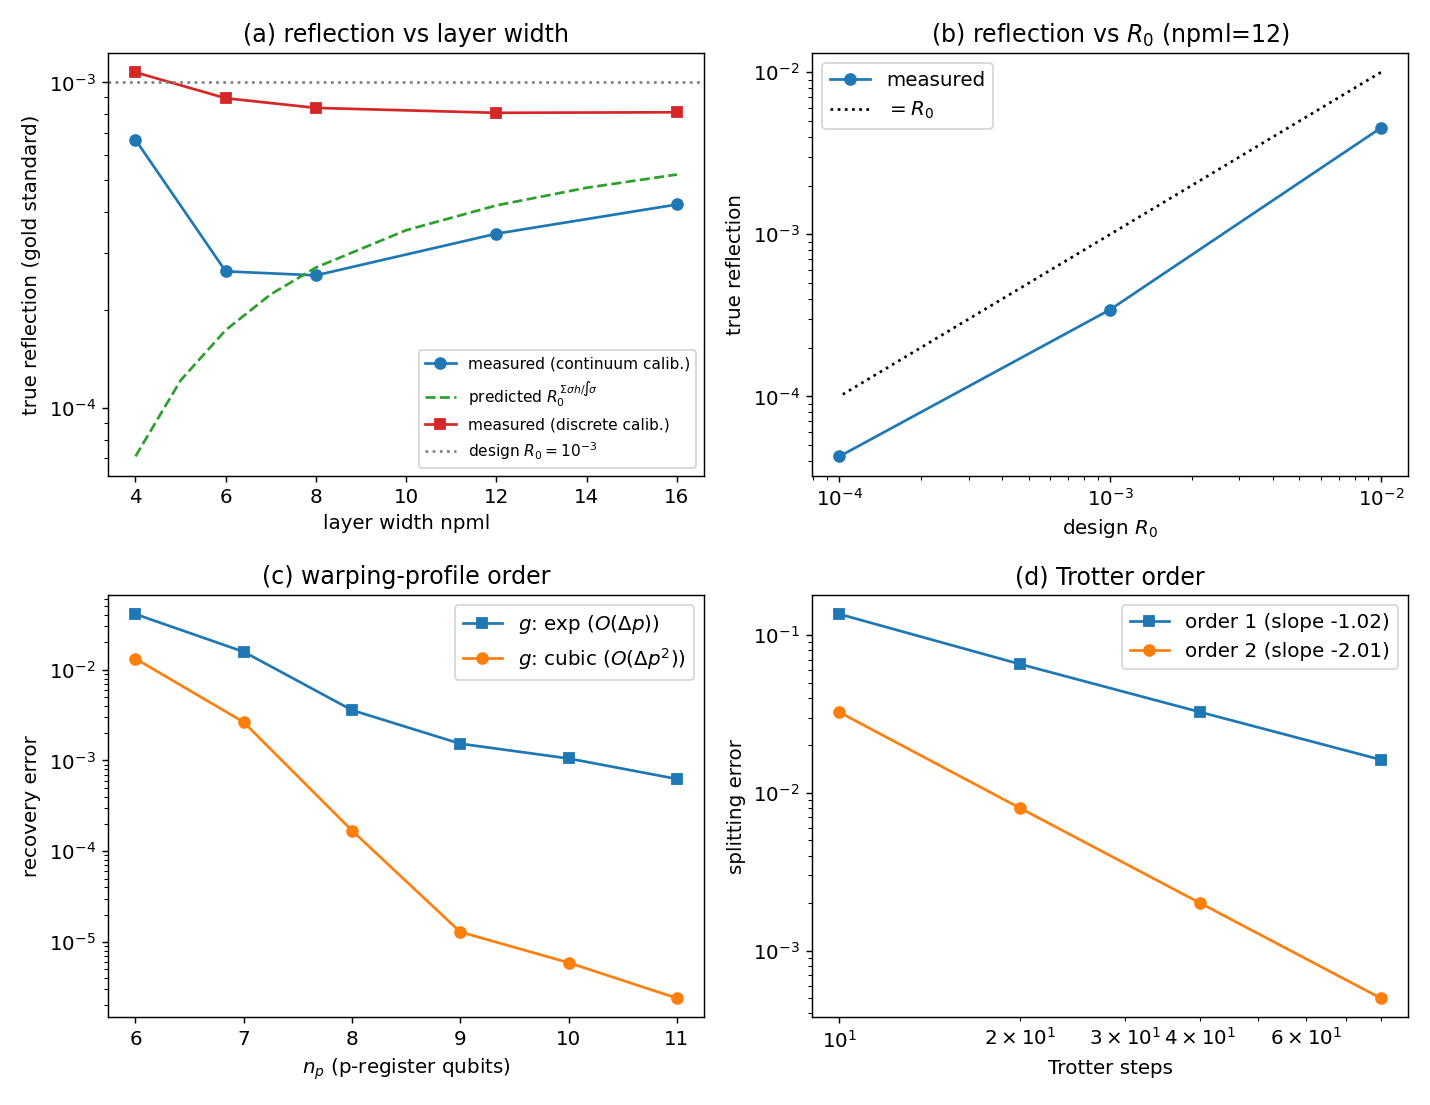
\includegraphics[width=\linewidth]{chapter3/paper_P1_convergence.png}
  \caption{Classical and Schr\"odingerisation convergence.
  (a)~Gold-standard reflection (truncated domain versus $4\times$
  reference) versus layer width $n_{\mathrm{pml}}$ at design reflection
  $R_0=10^{-3}$.  The curve is non-monotonic: the transition error falls
  with layer width while the wall return rises toward the design $R_0$
  from below, because node sampling of the polynomial profile
  over-damps thin layers (dashed curve: the predicted discrete
  wall-return $R_{\mathrm{eff}}=R_0^{\,\Sigma\sigma
  h/\!\int\!\sigma}$, which the measurement tracks within
  $5$--$20\%$ for $n_{\mathrm{pml}}\ge8$).  Red squares: the
  discretely calibrated profile pair (Appendix~\protect\ref{ch3:appD:validation}),
  for which the realised reflection is flat at the design value.
  (b)~Reflection versus $R_0$ at $n_{\mathrm{pml}}=12$: the measured
  reflection tracks the Collino--Tsogka design value within a factor
  ${\sim}2.3$ over two decades.
  (c)~Recovery error versus $p$-register size $n_p$ for the kinked
  $e^{-|p|}$ warping profile [$O(\Delta p)$] and the $C^{1}$ cubic
  profile [$O(\Delta p^{2})$] of Ref.~\protect\cite{jin2024recovery}, 1D CPML
  benchmark.
  (d)~Trotter splitting error versus step count at orders 1 and 2
  (fitted slopes $-1.02$ and $-2.01$), measured against the exact
  Schr\"odingerised evolution to isolate the splitting error.}
  \label{ch3:fig:convergence}
\end{figure}

\subsubsection{The recovery-threshold obstruction}
\label{ch3:sec:lemma}

The memory form pays a price.  The injection column ($\gamma$ on one
side) and the memory-source row ($\sigma\partial_x/\gamma$ on the other)
of each memory field are structurally asymmetric, and this asymmetry
cannot be scaled away.  Throughout this section
$\beta_j = \sigma_j/\kappa_j+\alpha_j\ge0$ denotes the CFS decay rate at
node $j$; we set the wave speed $c=1$ (so the stencil entries obey
$|D_{ji}|=1/h$), the general rate restoring a factor of $c$.

% Reconciled 2026-06-11: the (w_i,phi_j) coupling is one-directional
% (A[w,phi]=0), so the entry s lands in H_1 as s/2 and the eigenvalue of
% [[0,s/2],[s/2,-beta]] is (sqrt(beta^2+s^2)-beta)/2 — both pairs are
% governed by the same f.  The lemma statement now matches the proof.
\begin{lemma}[diagonal irreducibility]
\label{ch3:lem:threshold}
Let $A$ be the memory-form CPML generator of Section~\ref{ch3:sec:2d} and let
$G=\diag(\gamma_j)>0$ be any diagonal rescaling of the memory fields.
Let $s_j$ denote the magnitude of the memory-source coupling
($s_j\sim\sigma_j/(\gamma_j h)$ for the difference stencil).  Then the
Hermitian part $H_1(G)$ of the rescaled generator satisfies
\begin{equation}
  \lamax\bigl(H_1(G)\bigr) \;\ge\;
  \max_j\, \max\bigl\{\, f(\gamma_j,\beta_j),\; g(s_j,\beta_j) \,\bigr\}
  \;>\; 0,
  \label{ch3:eq:lemmabound}
\end{equation}
with $f(\gamma,\beta) = \bigl(\sqrt{\beta^{2}+\gamma^{2}}-\beta\bigr)/2$,
arising from the $2\times2$ principal submatrix
$\bigl[\begin{smallmatrix} 0 & \gamma/2 \\ \gamma/2 & -\beta
\end{smallmatrix}\bigr]$
on a $(v_j,\phi_j)$ pair by Cauchy interlacing, and
$g(s,\beta) = f(s,\beta)$ from a $(w_i,\phi_j)$ pair (the one-directional
coupling entry $s$ enters $H_1$ as $s/2$, so both pairs are governed by
the same $f$).  Optimising $\gamma$ against the two bounds gives
\begin{equation}
  \lamax(H_1) \;=\; \Theta\!\left(\sqrt{\sigma_{\max}\,c/h}\right)
  \qquad \text{as } h\to0,
  \label{ch3:eq:lemmarate}
\end{equation}
independent of the scaling.
\end{lemma}

The full proof is given in Appendix~\ref{ch3:app:proof}.  Its consistency
check is instructive: the collapsed 1D form of Section~\ref{ch3:sec:1d} has
\emph{no} injection pair (the memory is eliminated and the damping is
diagonal), so the lemma does not apply---and indeed
$H_1=-\diag(\sigma)\preceq0$ there.

\emph{Consequence.}  By the threshold of Eq.~\eqref{ch3:eq:recovery}
\cite[Thm.~3.1]{jin2024recovery}, recovery requires
$p^{*}\ge\lambda^{+}T$ with $\lambda^{+}\equiv\lamax^{+}(H_1)$, and the
post-selection probability of the recovery window scales as
$e^{-2p^{*}} = e^{-2\lambda^{+}T}$.  Numerically: at $\sigma_{\max}=0.5$
on an $8\times8$ grid, $\lambda^{+}=0.683$; recovery below the threshold
is $O(1)$ wrong, while above it the error drops to $2\times10^{-3}$
relative ($10^{-4}$ with $n_p=11$); see \ref{ch3:fig:threshold}.  The
sponge/CAP alternative (diagonal damping $\sigma_x+\sigma_y$, four
blocks) has $H_1\preceq0$ unconditionally at the price of matched-layer
quality.

% ----------------------------------------------------------------------
% CPML versus sponge at matched resources (end of Sec. III "The
% recovery-threshold obstruction"; replaces the [[CPML vs sponge at
% matched resources --- pending sweeps]] todo).
% Source of every number: paper/experiments/cpml_vs_sponge.py
%   -> paper/experiments/cpml_vs_sponge_results.json (run 2026-06-11).
% Labels prefixed cmp: to avoid collisions.
% ----------------------------------------------------------------------

\emph{CPML versus sponge at matched resources.}  A matched-resource
sweep quantifies this tradeoff: both absorbers on the same $32\times32$
grid with equal layer widths $n_{\mathrm{pml}}\in\{4,8,12\}$ and
default parameters, each measured against one shared $4\times$ enlarged
($128\times128$) hard-wall reference by the gold-standard protocol of
Section~\ref{ch3:sec:2d}, the reflection being the maximum interior error over
$T\in\{8,16,24,32,40\}$ (\ref{ch3:cmp:tab:matched}).  At equal layer
budget the CPML reaches its discrete wall-return level of
$2.7\times10^{-4}$ by $n_{\mathrm{pml}}=8$ [consistent with the
$2.8\times10^{-4}$ gold-standard value of Section~\ref{ch3:sec:2d}], while the
sponge stays at the percent level, improving only from
$6.2\times10^{-2}$ to $3.6\times10^{-2}$ across the sweep---a quality
gap of a factor of $170$ at $n_{\mathrm{pml}}=8$ ($130$ at $12$).  The
quantum-side cost inverts the ranking.  The sponge has $\lambda^{+}=0$
exactly, so its recovery post-selects at the $T$-independent
$e^{2p^{*}}\approx1.2$ (default slice $p^{*}\approx0.11$); the CPML
pays $e^{2\lambda^{+}T}$, with $\lambda^{+}=0.93$--$1.54$ tracking the
$\Theta(\sqrt{\sigma_{\max}c/h})$ rate of Lemma~\ref{ch3:lem:threshold} to
within $5\%$---already $7\times10^{7}$ at $T=8$ and $1.6\times10^{39}$
at $T=40$ for $n_{\mathrm{pml}}=8$.  Neither absorber dominates at
matched resources: the sponge trades two orders of magnitude in
reflection for an essentially free recovery, and the CPML trades an
exponentially growing post-selection penalty for matched-layer
accuracy---precisely the penalty that the symmetrizer of
Section~\ref{ch3:sec:symmetrizer} replaces by a $T$-independent conditioning
factor.

\begin{table}[tb]
\caption{CPML versus sponge at matched resources: $32\times32$ grid,
equal layer width $n_{\mathrm{pml}}$, default parameters [$m=2$,
$R_0=10^{-3}$, Collino--Tsogka amplitudes
$\sigma_{\max}=2.59/1.30/0.86$ at $n_{\mathrm{pml}}=4/8/12$].
Reflection is the gold-standard interior error against a single shared
$4\times$ enlarged ($128\times128$) hard-wall reference, maximised over
$T\in\{8,16,24,32,40\}$ ($\lVert z_0\rVert=1$).
$\lambda^{+}=\lamax^{+}(H_1)$ sets the CPML post-selection penalty
$e^{2\lambda^{+}T}$ (quoted at $T=40$) and tracks
$\sqrt{\sigma_{\max}}$ to within $5\%$; the sponge has
$\lambda^{+}=0$, post-selecting at the $T$- and
$n_{\mathrm{pml}}$-independent $e^{2p^{*}}=1.2$ for the default
recovery slice $p^{*}=0.11$.}
\label{ch3:cmp:tab:matched}
\begin{tabular}{lllll}
\toprule
 & \multicolumn{2}{c}{Reflection (max over $T$)} &
   \multicolumn{2}{c}{CPML recovery cost} \\
\cline{2-3}\cline{4-5}
$n_{\mathrm{pml}}$ & CPML & sponge & $\lambda^{+}(H_1)$ &
$e^{2\lambda^{+}T}$, $T{=}40$ \\
\midrule
4  & $4.2\times10^{-3}$ & $6.2\times10^{-2}$ & 1.54 & $2.2\times10^{53}$ \\
8  & $2.7\times10^{-4}$ & $4.7\times10^{-2}$ & 1.13 & $1.6\times10^{39}$ \\
12 & $2.8\times10^{-4}$ & $3.6\times10^{-2}$ & 0.93 & $1.5\times10^{32}$ \\
\bottomrule
\end{tabular}
\end{table}


\begin{figure}
  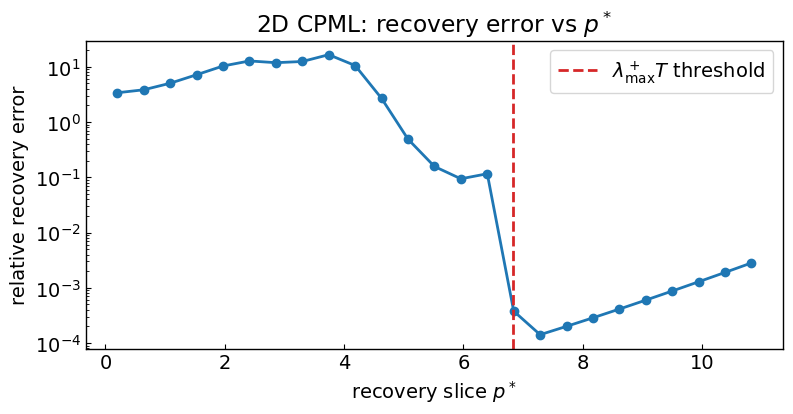
\includegraphics[width=\linewidth]{chapter3/fig4_2d_recovery_threshold.png}
  \caption{The recovery threshold in action (2D CPML, $8\times8$ grid,
  $\sigma_{\max}=0.5$, $T=10$).  Relative recovery error versus the slice
  position $p^{*}$: below the threshold $p^{*}=\lambda^{+}T$ (dashed
  line, $\lambda^{+}=0.683$) the recovered state is $O(1)$ wrong; just
  above it the error drops by four orders of magnitude, then grows
  slowly as $e^{p^{*}}$ amplifies the $p$-grid discretisation floor.}
  \label{ch3:fig:threshold}
\end{figure}

\subsubsection{The Lyapunov symmetrizer}
\label{ch3:sec:symmetrizer}

A matrix $W>0$ solving the Lyapunov inequality
$WA + A^{\dagger}W\preceq0$ gives, with $S=W^{1/2}$, a transformed
generator $\At = SAS^{-1}$ whose Hermitian part satisfies
\begin{equation}
  \Ht \;=\; \tfrac12\, S^{-1}\bigl(WA + A^{\dagger}W\bigr)S^{-1}
  \;\preceq\; 0
  \label{ch3:eq:congruence}
\end{equation}
by congruence.  Recovery of $\tilde z = Sz$ is then valid at any
$p^{*}>0$, and $z = S^{-1}\tilde z$ is recovered classically (or folded
into the readout).  Since $A$ is only marginally stable (interior modes
are neutral), we construct $W$ from the $\epsilon$-shifted generator:
\begin{equation}
  A_\epsilon = A - \epsilon I, \qquad
  A_\epsilon^{\dagger}W + WA_\epsilon = -I, \qquad
  S = W^{1/2},
  \label{ch3:eq:lyapunov}
\end{equation}
the shift being undone classically by the factor $e^{\epsilon T}$.  An
exact identity follows (Proposition~\ref{ch3:appE:prop} in
Appendix~\ref{ch3:appE:symmetrizer}: congruence gives
$\mathrm{Herm}(SA_\epsilon S^{-1})=-W^{-1}/2$ exactly; verified to better
than $10^{-11}$ relative in all 18 measured configurations): the
transform of the \emph{original} $A$ has
\begin{equation}
  \lamax(\Ht) \;=\; \epsilon - \frac{1}{2\lamax(W)} \;\approx\; \epsilon,
  \label{ch3:eq:identity}
\end{equation}
while the transform of $A_\epsilon$ has $\Ht\preceq0$ strictly.  We
therefore use the shifted transform; the undo factor
$e^{\epsilon T}\le e^{0.4}$ over the horizons tested is trivial.

\begin{table}
\caption{Lyapunov-symmetrizer conditioning across all measured
configurations [grids $(n_x,n_y)$ qubits per dimension, i.e.\ $8\times8$,
$16\times8$, $16\times16$ points; $n$ is the full state dimension
including the eight blocks].  $\lambda^{+}=\lamax^{+}(H_1)$ is the
indefiniteness of the untransformed generator;
$\kappa_2(S)=\sqrt{\operatorname{cond}_2(W)}$ the conditioning of the
symmetrizer; $\lamax(\Ht^{(\epsilon)})$ the (strictly negative) largest
Hermitian-part eigenvalue of the $\epsilon$-shifted transform
$SA_\epsilon S^{-1}$; and $T^{*}=\ln\kappa^{2}/(2\lambda^{+})$ the
crossover time beyond which the symmetrizer beats the direct
above-threshold recovery.  All Lyapunov residuals are
$\le1.4\times10^{-14}$ (relative).}
\label{ch3:tab:kappa}
\begin{tabular}{llllllll}
\toprule
Grid & $n$ & $\sigma_{\max}$ & $\epsilon$ & $\lambda^{+}(H_1)$ &
$\kappa_2(S)$ & $\lamax(\Ht^{(\epsilon)})$ & $T^{*}$ \\
\midrule
$8\times8$ & 512 & 0.5 & $10^{-2}$ & 0.683 & $4.0\times10^{2}$ & $-4.6\times10^{-6}$ & 8.8 \\
$8\times8$ & 512 & 0.5 & $10^{-3}$ & 0.683 & $3.0\times10^{3}$ & $-8.1\times10^{-8}$ & 11.7 \\
$8\times8$ & 512 & 0.5 & $10^{-4}$ & 0.683 & $1.1\times10^{4}$ & $-6.0\times10^{-9}$ & 13.6 \\
$8\times8$ & 512 & 1.0 & $10^{-2}$ & 0.927 & $5.1\times10^{2}$ & $-5.2\times10^{-6}$ & 6.7 \\
$8\times8$ & 512 & 1.0 & $10^{-3}$ & 0.927 & $2.9\times10^{3}$ & $-1.6\times10^{-7}$ & 8.6 \\
$8\times8$ & 512 & 1.0 & $10^{-4}$ & 0.927 & $9.8\times10^{3}$ & $-1.4\times10^{-8}$ & 9.9 \\
$16\times8$ & 1024 & 0.5 & $10^{-2}$ & 0.687 & $5.1\times10^{2}$ & $-3.0\times10^{-6}$ & 9.1 \\
$16\times8$ & 1024 & 0.5 & $10^{-3}$ & 0.687 & $7.0\times10^{3}$ & $-1.5\times10^{-8}$ & 12.9 \\
$16\times8$ & 1024 & 0.5 & $10^{-4}$ & 0.687 & $3.1\times10^{4}$ & $-8.0\times10^{-10}$ & 15.0 \\
$16\times8$ & 1024 & 1.0 & $10^{-2}$ & 0.956 & $7.5\times10^{2}$ & $-2.4\times10^{-6}$ & 6.9 \\
$16\times8$ & 1024 & 1.0 & $10^{-3}$ & 0.956 & $7.0\times10^{3}$ & $-2.8\times10^{-8}$ & 9.3 \\
$16\times8$ & 1024 & 1.0 & $10^{-4}$ & 0.956 & $2.7\times10^{4}$ & $-1.8\times10^{-9}$ & 10.7 \\
$16\times16$ & 2048 & 0.5 & $10^{-2}$ & 0.694 & $5.7\times10^{2}$ & $-2.4\times10^{-6}$ & 9.1 \\
$16\times16$ & 2048 & 0.5 & $10^{-3}$ & 0.694 & $9.9\times10^{3}$ & $-7.7\times10^{-9}$ & 13.3 \\
$16\times16$ & 2048 & 0.5 & $10^{-4}$ & 0.694 & $6.6\times10^{4}$ & $-1.7\times10^{-10}$ & 16.0 \\
$16\times16$ & 2048 & 1.0 & $10^{-2}$ & 0.972 & $8.6\times10^{2}$ & $-1.9\times10^{-6}$ & 6.9 \\
$16\times16$ & 2048 & 1.0 & $10^{-3}$ & 0.972 & $1.2\times10^{4}$ & $-8.7\times10^{-9}$ & 9.7 \\
$16\times16$ & 2048 & 1.0 & $10^{-4}$ & 0.972 & $6.3\times10^{4}$ & $-3.4\times10^{-10}$ & 11.4 \\
\bottomrule
\end{tabular}
\end{table}

\begin{table}
\caption{End-to-end recovery tradeoff: direct versus symmetrized
recovery, errors
$\lVert z_{\mathrm{rec}}-e^{AT}z_0\rVert_2/\lVert e^{AT}z_0\rVert_2$.
``Small $p^{*}$'' is the library-default slice three grid points above
zero.  For the untransformed system above threshold,
$p^{*}=\lambda^{+}T+1$ and the post-selection penalty is $e^{2p^{*}}$;
entries marked ``--'' exceed the $p$-domain
($\lambda^{+}T+1>p_{\max}$).  The symmetrized column uses the
$\epsilon$-shifted transform at $\epsilon=10^{-3}$ recovered at the same
small $p^{*}$, with the $T$-independent penalty
$\kappa_2^{2}(S)$ of \protect\ref{ch3:tab:kappa}.  The $16\times16$ run uses a
reduced $p$ register ($n_p=8$), which sets its higher error floor.}
\label{ch3:tab:tradeoff}
\resizebox{\linewidth}{!}{%
\begin{tabular}{llllllll}
\toprule
 & & \multicolumn{4}{c}{Untransformed} & \multicolumn{1}{c}{Symmetrized ($\epsilon=10^{-3}$)} \\
\cline{3-6}\cline{7-7}
Configuration & $T$ & err.\ (small $p^{*}$) & $p^{*}\!\ge\!\lambda^{+}T$ &
err.\ (above thr.) & penalty $e^{2p^{*}}$ & err.\ (small $p^{*}$) \\
\midrule
$8\times8$ ($\sigma_{\max}=0.5$, $n_p=11$) & 10 & $3.4$ & 7.8 & $1.2\times10^{-4}$ & $6.3\times10^{6}$ & $1.2\times10^{-6}$ \\
 & 20 & $8.3$ & 14.7 & $2.4\times10^{-1}$ & $5.4\times10^{12}$ & $2.4\times10^{-6}$ \\
 & 40 & $2.6\times10^{1}$ & -- & -- & -- & $4.4\times10^{-6}$ \\
$8\times8$ ($\sigma_{\max}=1.0$, $n_p=11$) & 10 & $7.2$ & 10.3 & $2.2\times10^{-2}$ & $8.4\times10^{8}$ & $2.1\times10^{-5}$ \\
 & 20 & $1.6\times10^{1}$ & 19.6 & $3.0\times10^{2}$ & $1.0\times10^{17}$ & $2.3\times10^{-5}$ \\
 & 40 & $2.9\times10^{1}$ & 38.1 & $7.3\times10^{15}$ & $1.2\times10^{33}$ & $3.5\times10^{-5}$ \\
$16\times8$ ($\sigma_{\max}=0.5$, $n_p=10$) & 10 & $2.5$ & 7.9 & $1.1\times10^{-4}$ & $7.4\times10^{6}$ & $4.2\times10^{-6}$ \\
 & 20 & $4.8$ & 14.8 & $4.5\times10^{-1}$ & $6.7\times10^{12}$ & $6.0\times10^{-6}$ \\
 & 40 & $1.3\times10^{1}$ & -- & -- & -- & $1.1\times10^{-5}$ \\
$16\times16$ ($\sigma_{\max}=0.5$, $n_p=8$) & 10 & $2.0$ & 8.0 & $1.3\times10^{-2}$ & $9.2\times10^{6}$ & $1.1\times10^{-4}$ \\
 & 20 & $5.6$ & 15.0 & $7.5\times10^{1}$ & $1.0\times10^{13}$ & $5.2\times10^{-4}$ \\
 & 40 & $2.5\times10^{1}$ & -- & -- & -- & $3.8\times10^{-3}$ \\
\bottomrule
\end{tabular}%
}
\end{table}

\emph{Measured results} [grids $8\times8$, $16\times8$, $16\times16$
($n=512$--$2048$), $\sigma_{\max}\in\{0.5,1.0\}$,
$\epsilon\in\{10^{-2},10^{-3},10^{-4}\}$; Lyapunov residuals
$\le1.4\times10^{-14}$; \ref{ch3:tab:kappa} and \ref{ch3:tab:tradeoff},
\ref{ch3:fig:symmetrizer}]:
\begin{itemize}
\item \emph{End-to-end recovery at the default small $p^{*}$}
  ($\epsilon=10^{-3}$): transformed errors
  $1.2\times10^{-6}$--$3.5\times10^{-5}$ on the configurations with
  $n_p\in\{10,11\}$, essentially flat in $T$ over $T\in\{10,20,40\}$; the
  $16\times16$ run with a reduced $p$ register ($n_p=8$) gives
  $1.1\times10^{-4}$--$3.8\times10^{-3}$, consistent with its
  $O(\Delta p^{2})$ floor.  The untransformed system at the same $p^{*}$
  returns $O(1)$--$O(10)$ garbage growing with $T$.
\item \emph{The direct above-threshold method is worse than its nominal
  $e^{2\lambda^{+}T}$ cost}: at $T=20$ it degrades (errors $0.24$--$0.45$
  at $\sigma_{\max}=0.5$) and at $T=40$ it explodes (error up to
  $7\times10^{15}$ at $p^{*}=38$) because $e^{p^{*}}$ amplifies the
  $p$-grid floor.  At long $T$ the symmetrizer is not merely cheaper---it
  is the only working recovery.
\item \emph{Conditioning}:
  $\kappa_2(S)=4.0\times10^{2}$--$8.6\times10^{2}$ at $\epsilon=10^{-2}$
  (the recommended setting), flat in $\sigma_{\max}$, scaling as
  ${\sim}\epsilon^{-0.6\,\text{to}\,-1.0}$---and \emph{saturating} in
  $n$: extending the measurement to $n=4096$ gives
  $\kappa_2(S)=564.5$ at $\epsilon=10^{-2}$ versus $566.9$ at $n=2048$
  (local slope $-0.006$; over the full range $n=512$--$4096$ the fitted
  power-law exponent drops from $0.25$ to $0.16$ with degrading fit
  quality, i.e.\ a power law is the wrong model because $\kappa$ is
  flattening).  $\lambda^{+}$ itself saturates ($0.683\to0.694$ over
  $8\times$ in $n$) and $\lambda_{\min}(W)$ stays at $0.66$--$0.68$, so
  the $\kappa$ growth is driven entirely by
  $\lambda_{\max}(W)\sim1/(2\epsilon)$: the conditioning is
  $\epsilon$-controlled, not grid-controlled, and the symmetrizer cost
  does not blow up under mesh refinement.  The eigenvector symmetrizer
  $W=(VV^{\dagger})^{-1}$ is four to six orders of magnitude worse
  conditioned ($\kappa_2\sim3\times10^{8}$) and fails outright on
  near-defective configurations---the Lyapunov route is the right
  construction.
\item \emph{Tradeoff}:
  $T^{*}=\ln\kappa^{2}/(2\lambda^{+})=6.7$--$16.0$ across all
  configurations; at $T=20$ the symmetrizer wins by 4--9 orders of
  magnitude in post-selection cost, at $T=40$ by 16--26 orders.  $T^{*}$
  grows only logarithmically with $\kappa$, hence very weakly with grid
  size.
\end{itemize}

\emph{Structure and compressibility of $S$.}  We measured the structure
of $S$ directly and tested 25 approximate symmetrizers (distance-banded,
magnitude-thresholded, block-pattern, identity-plus-low-rank, hybrid,
and inverse-side-banded families) for dissipativity and end-to-end
recovery on the $n=512$ and $n=1024$ systems.  Three findings.
(i)~Identity-plus-low-rank is \emph{ruled out}: the correction
$E=S-\alpha I$ is numerically full rank (995 of 1024 singular values
above $10^{-2}$ of the top), and $\lamax(\tilde H_1)$ stays at the
\emph{untransformed} $\lambda^{+}=0.67$ for ranks $8$--$64$---no
few-term LCU implementation of $S$ exists.  (ii)~Strict sparsification
preserving $\lamax(\tilde H_1)\le\epsilon$ requires essentially the
full active support ($\approx48$--$51\%$ of entries; on the remaining
``dead'' indices---interior memory and padding, $30$--$50\%$ of the
space---$S$ is exactly a multiple of the identity, which is free
structure).  (iii)~\emph{Moderate compression works} once the residual
$\lambda_b$ of an approximate $S_b$ is absorbed as an additional shift
(undone by $e^{\lambda_b T}\le e^{2.6}\approx14$ at the worst measured
$\lambda_b=0.066$, $T=40$): magnitude thresholding at $35\%$ density
recovers to $8.7\times10^{-6}$ ($T=10$) and $5.4\times10^{-5}$
($T=40$); a rank-$32$-plus-band-$8$ hybrid at $26\%$ reaches
$1.3\times10^{-5}$ and $6.6\times10^{-4}$ (all $n=1024$; the
conditioning of every usable $S_b$ stays ${\sim}5\times10^{2}$, equal
to the exact $S$).  The energy of $E$ is $99.6\%$ concentrated on
layer-strip index pairs.  The implementation route is therefore
block-encoding of a ${\sim}35\%$-dense operator (times the free
dead-index identity factor), not a local circuit or a short LCU; at
current theory the symmetrizer is best used as classical pre/\allowbreak
post-processing, and a structured-ansatz Lyapunov construction (solving
for $W$ within a polynomially parametrised operator family) is the open
problem these measurements sharpen.

\emph{Honest limitations.}  The construction requires a dense $O(n^{3})$
classical precomputation of $W$, $S$, $S^{-1}$; the fate of the sparse
quantised-tensor-train (QTT) term structure under the dense similarity
(Trotter circuits for $\At$) is not assessed; the $\kappa$ scaling
beyond $n=4096$ is extrapolation (though saturating); the compression
study is at $n\le1024$.

\begin{figure}
  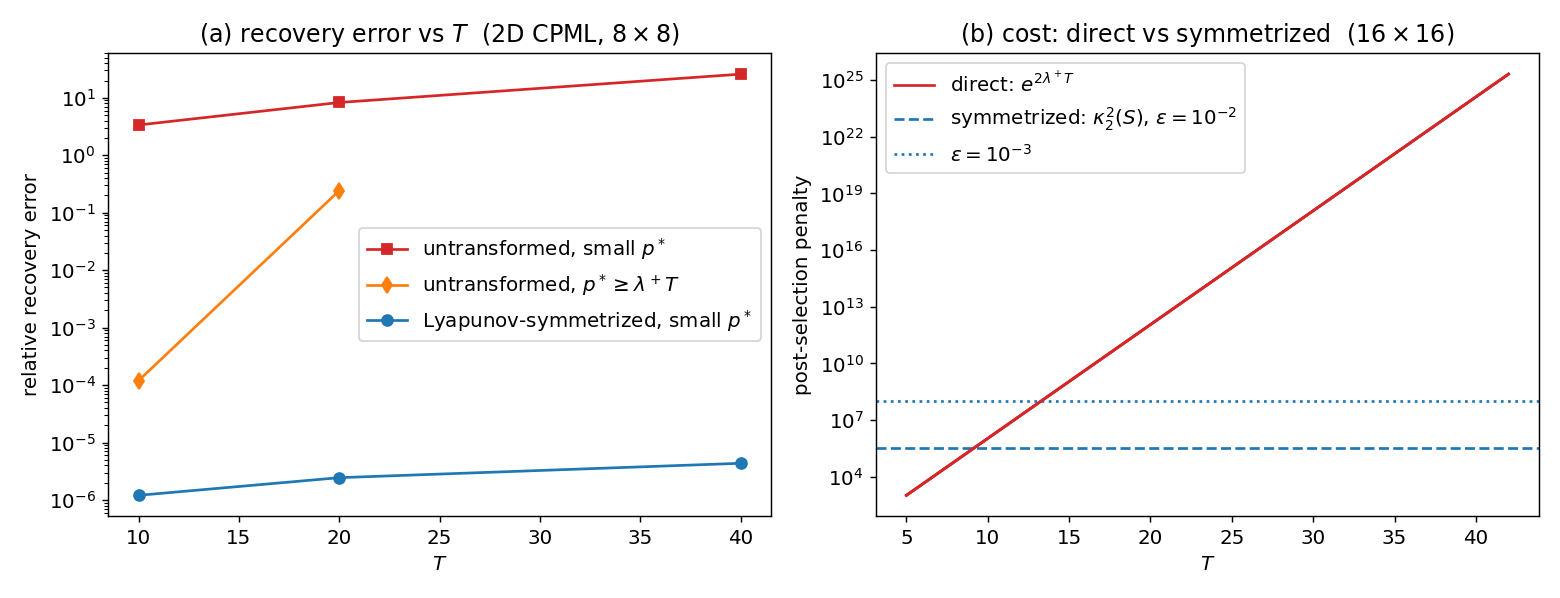
\includegraphics[width=\linewidth]{chapter3/paper_P2_symmetrizer.png}
  \caption{The Lyapunov symmetrizer.  (a)~Relative recovery error versus
  evolution time $T$ for the 2D CPML system ($8\times8$ grid,
  $\sigma_{\max}=0.5$): untransformed recovery at the default small
  $p^{*}$ (squares) is $O(1)$ garbage; untransformed recovery above the
  threshold $p^{*}\ge\lambda^{+}T$ (diamonds) degrades with $T$ as
  $e^{p^{*}}$ amplifies the $p$-grid floor and leaves the admissible
  $p$-domain entirely by $T=40$; the Lyapunov-symmetrized recovery at the
  same small $p^{*}$ (circles, $\epsilon=10^{-3}$, shifted transform)
  stays at the $10^{-6}$ level, essentially flat in $T$.
  (b)~Post-selection cost on the $16\times16$ grid: the direct
  $e^{2\lambda^{+}T}$ penalty (solid) against the $T$-independent
  symmetrizer penalty $\kappa_2^{2}(S)$ at $\epsilon=10^{-2}$ (dashed)
  and $10^{-3}$ (dotted); the crossovers are the $T^{*}$ values of
  \protect\ref{ch3:tab:kappa}.}
  \label{ch3:fig:symmetrizer}
\end{figure}

% ======================================================================
\subsection{Explicit circuits}
\label{ch3:sec:circuits}

\subsubsection{Projector-extended Bell-basis term evolution}
\label{ch3:sec:projector}

The circuit of Sato \emph{et al.}~\cite{sato2024hamiltonian}
exponentiates ladder-string terms (alphabet $\{I,\sigma_{01},
\sigma_{10}\}$) via a Bell-basis change followed by one multi-controlled
$R_z$; Hu, Jin, Liu, and Zhang~\cite{hu2024quantum} extended the
framework to non-unitary PDE dynamics via Schr\"odingerisation, and Jin,
Liu, and Yu~\cite{jin2024heat} built gate-level circuits for the heat
equation with physical boundaries.  Relative to these we add the
\emph{projector} extension: strings containing
$z=\lvert0\rangle\langle0\rvert$ and $o=\lvert1\rangle\langle1\rvert$
(block projectors of separated multi-field systems) enter as plain
$0$-/$1$-controls; the Bell rotation outside the projected subspace is
undone exactly, so the circuit implements
$e^{-i\,\delta t\,(cP+\mathrm{h.c.})}$ for projector-valued $P$.
\ref{ch3:fig:circuits}(a) shows the compiled circuit for a
representative projector-containing term of the separated 2D wave
Hamiltonian, and \ref{ch3:fig:circuits}(b) the full Schr\"odingerised
pipeline it slots into.

\begin{figure}[tb]
  \centering
  \makebox[0pt][r]{(a)\hspace{0.96\linewidth}}\\[-0.5ex]
  \resizebox{\linewidth}{!}{%
  \begin{quantikz}[row sep={0.62cm,between origins}, column sep=0.22cm]
    \lstick{$q_0\;(\sigma_{10})$} & \qw & \targ{} & \qw & \qw
      & \ctrl{1} & \qw & \qw & \targ{} & \qw & \qw \\
    \lstick{$q_1\;(\sigma_{01})$} & \targ{} & \qw & \qw & \qw
      & \octrl{3} & \qw & \qw & \qw & \targ{} & \qw \\
    \lstick{$q_2\;(I)$} & \qw & \qw & \qw & \qw
      & \qw & \qw & \qw & \qw & \qw & \qw \\
    \lstick{$q_3\;(I)$} & \qw & \qw & \qw & \qw
      & \qw & \qw & \qw & \qw & \qw & \qw \\
    \lstick{$q_4\;(\sigma_{00})$} & \qw & \qw & \qw & \qw
      & \octrl{1} & \qw & \qw & \qw & \qw & \qw \\
    \lstick{$q_5\;(\sigma_{01},\,\mathrm{piv.})$}
      & \ctrl{-4} & \ctrl{-5} & \gate{P(\lambda)} & \gate{H}
      & \gate{R_z(2\gamma\,\delta t)} & \gate{H} & \gate{P(-\lambda)}
      & \ctrl{-5} & \ctrl{-4} & \qw
  \end{quantikz}}\\[1.2ex]
  \makebox[0pt][r]{(b)\hspace{0.96\linewidth}}\\[-0.5ex]
  \resizebox{\linewidth}{!}{%
  \begin{quantikz}[row sep={0.95cm,between origins}, column sep=0.18cm]
    \lstick{sys} & \qwbundle{n_s} & \gate{\lvert\psi_0\rangle} & \qw
      & \gate[2]{e^{+i\frac{\Delta t}{2}\eta\Sigma}}
      & \gate{e^{-i\Delta t H}}
      & \gate[2]{e^{+i\Delta t\,\eta\Sigma}}
      & \ \ldots\
      & \gate{e^{-i\Delta t H}}
      & \gate[2]{e^{+i\frac{\Delta t}{2}\eta\Sigma}}
      & \qw & \qw \\
    \lstick{$p$} & \qwbundle{n_p} & \gate{\lvert g\rangle}
      & \gate{\mathrm{QFT}^{\dagger}} & {} & \qw & {}
      & \ \ldots\
      & \qw & {} & \gate{\mathrm{QFT}} & \meter{p^{*}}
  \end{quantikz}}
  \caption{Explicit circuits.  (a)~Bell-basis evolution
  $e^{-i\,\delta t\,(cP+\mathrm{h.c.})}$ of the projector-containing
  term $P=\sigma_{01}\otimes\sigma_{00}\otimes I\otimes I\otimes
  \sigma_{01}\otimes\sigma_{10}$ of the separated 2D wave Hamiltonian
  (string \texttt{mzIImp}, qubit $q_k$ carrying string character $5-k$;
  $\lambda=\arg c$, $\gamma=|c|$; $\lambda=0$ for the real wave-equation
  coefficients): \textsc{cnot}s rotate the ladder qubits to the Bell
  basis, and the single multi-controlled $R_z$ carries the block
  projector $\sigma_{00}$ ($q_4$) as an \emph{open-circle}
  $0$-control---the entire compilation rule of
  Section~\protect\ref{ch3:sec:projector}.  The gate sequence is unitarily identical to
  the library-compiled circuit (verified to machine precision).
  (b)~The Schr\"odingerised pipeline (Section~\protect\ref{ch3:sec:circuit}) on bundled
  registers: product-state preparation
  $\lvert g\rangle\otimes\lvert\psi_0\rangle$, $\mathrm{QFT}^{\dagger}$
  on the $p$ register, Strang-split steps alternating the Bell wave
  circuit $e^{-i\Delta t H}$ with the diagonal damping phases
  $e^{+i\Delta t\,\eta\Sigma}$ (half steps at the ends), closing
  $\mathrm{QFT}$, and recovery by measuring the $p$ register,
  post-selecting the slice at $p^{*}$, and rescaling classically by
  $e^{p^{*}}$.}
  \label{ch3:fig:circuits}
\end{figure}

Due diligence (full-text check of both papers): neither
Ref.~\cite{hu2024quantum} nor Ref.~\cite{jin2024heat} circuitises
projector-containing strings---both use only the
$\{I,\sigma_{01},\sigma_{10}\}$ alphabet.  We confirmed this at code
level in the published companion notebook of
Ref.~\cite{hu2024quantum}: its term circuit ($W_j$) implements the
contiguous ladder pattern with rotations controlled uniformly on all
lower qubits (an all-or-nothing $X$-conjugation flag serving the
periodic corner terms), with no per-qubit $0$-/$1$-control selection
(the nilpotent shift needs no
projector guards in scalar single-field problems, and
Ref.~\cite{jin2024heat} routes boundary data into source terms precisely
to avoid non-Toeplitz structure).  Ref.~\cite{sato2025nonconservative}
comes closest: its symbolic operator algebra over
$\{I,\sigma_{00},\sigma_{11},\sigma_{01},\sigma_{10}\}$ produces
projector factors from boundary-truncated shifts and piecewise-constant
coefficients, and poly-depth Trotterisation is asserted by citation to
Ref.~\cite{sato2024hamiltonian}; but no gate-level compilation rule for
the projector factors and no projector-term circuit is given.  A caveat
we state explicitly: the
abstract class $\lvert a\rangle\langle b\rvert + \lvert b\rangle\langle
a\rvert$ over basis states in Lemma~1 of
Refs.~\cite{sato2024hamiltonian,hu2024quantum} implicitly \emph{contains}
Hermitian-paired projector strings as an existence statement; our
contribution is the explicit alphabet extension and compilation rule
(projector factor $\to$ $0$-/$1$-control) and its application to
multi-field block-coupled systems, not a new diagonalisation principle.
The extension is backward compatible.  Unitary-level validation: the
error is pure per-step Trotter error $0.50\,\delta t^{2}$ with no phase
offset.  This unlocks the separated 2D wave Hamiltonian
(\texttt{zm}/\texttt{mz} block couplings) needed for per-direction
absorbing layers.

\subsubsection{The Schr\"odingerised circuit}
\label{ch3:sec:circuit}

The full pipeline is
\begin{equation}
\begin{split}
  \mathrm{init}(g\otimes\psi_0)
  \;\to\; \mathrm{QFT}^{\dagger}_p
  \;\to\; [\text{Trotter steps}] \\
  \;\to\; \mathrm{QFT}_p
  \;\to\; \text{slice at } p^{*}.
\end{split}
  \label{ch3:eq:pipeline}
\end{equation}
Each step (diagonal $H_1$) factorises into the wave circuit (the Bell
construction of Section~\ref{ch3:sec:projector} on the system register) and a
diagonal damping phase with entries $e^{+i\,\delta t\,\eta_k\sigma_j}$.
Both Trotter levels are symmetrised (Strang outer; palindromic term order
inner), with measured clean second order: errors
$4\times10^{-2}\to10^{-2}\to2.7\times10^{-3}$ at $50/100/200$ steps on 17
qubits.

\emph{Fitted orders} [1D benchmark, error versus the exact
Schr\"odingerised evolution to isolate the splitting;
\ref{ch3:fig:convergence}(d)]: slope $-1.02$ (order~1), $-2.01$ (order~2
with both levels symmetrised); against the full matrix-exponential
reference the order-2 error saturates at the $p$-discretisation floor, as
expected.  \emph{Warping-profile order} [recovery error versus $n_p$,
fixed 1D PML case; \ref{ch3:fig:convergence}(c)]: $e^{-|p|}$ slope
${\sim}{-1}$ in $\Delta p$ ($4.1\times10^{-2}\to6.3\times10^{-4}$ over
$n_p=6$--$11$); $C^{1}$ cubic ${\sim}{-2}$
($1.3\times10^{-2}\to2.4\times10^{-6}$), confirming Remark~4.9 of
Ref.~\cite{jin2024recovery} in this setting.

\subsubsection{End-to-end demonstrations}
\label{ch3:sec:demos}

\begin{itemize}
\item 1D CPML, 14 qubits (6 system $+$ 8 $p$), 60 steps, $T=30$:
  recovered solution within $7\times10^{-4}$ of the exact non-unitary
  evolution.
\item 2D sponge, $8\times8$ grid, 17 qubits, $T=10$:
  $2.7\times10^{-3}$ at 200 steps (\ref{ch3:fig:gate17}).
\item 2D sponge, $32\times32$ grid, 21 qubits (12 system $+$ 9 $p$), up
  to 240 steps (983 native operations per step): errors
  $7.7\times10^{-3}$ / $1.7\times10^{-2}$ / $1.4\times10^{-2}$ at
  $T=8/16/24$; energy decays from $0.97$ to $1.25\times10^{-3}$
  (absorption complete); nine minutes of statevector simulation
  (\ref{ch3:fig:gate21}).
\end{itemize}
Qubit accounting: the absorbing overhead is $+1$ (sponge) or $+2$ (CPML)
block qubits plus $n_p\approx8$--$10$ for the $p$ register; $n_p$ depends
only logarithmically on $T$, the damping rate, and the target accuracy.

\begin{figure}
  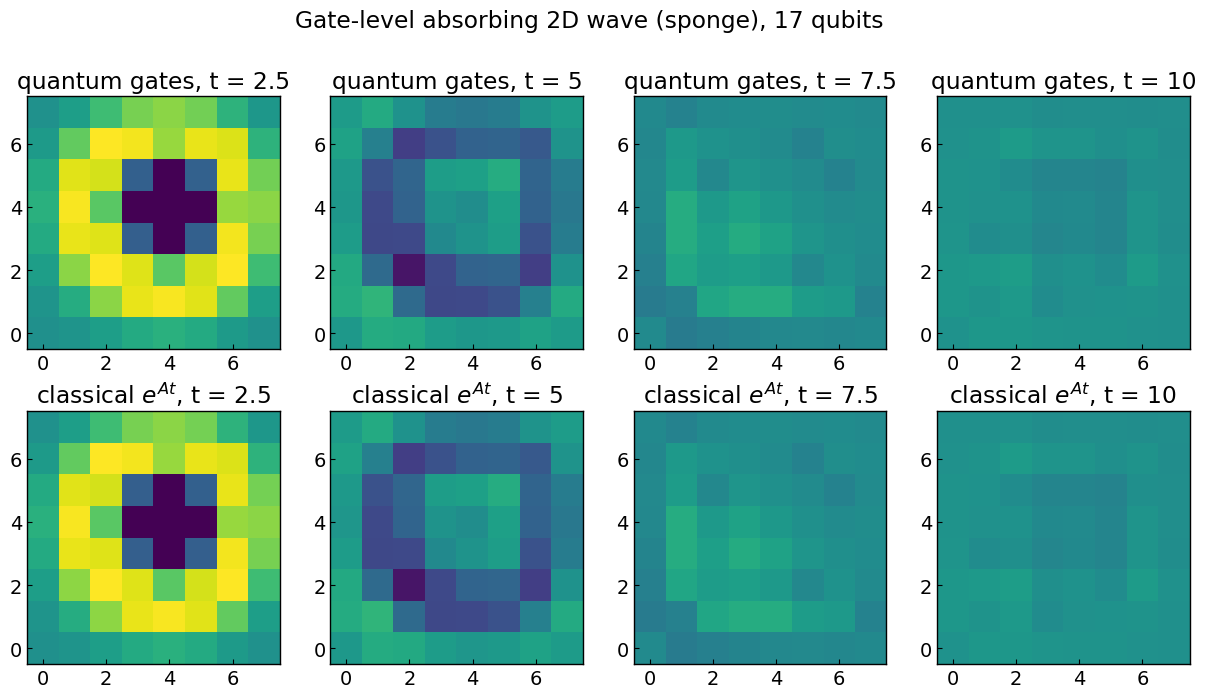
\includegraphics[width=\linewidth]{chapter3/fig5_2d_gate_level_simulation.png}
  \caption{Gate-level absorbing 2D wave evolution (sponge layer,
  $8\times8$ grid, 17 qubits $=$ 6 grid $+$ 2 block $+$ 9 $p$-register).
  Top row: snapshots of the recovered field from the Trotterised quantum
  circuit at $t=2.5,5,7.5,10$.  Bottom row: the exact non-unitary
  reference $e^{At}\psi_0$.  The expanding pulse is absorbed in the
  boundary layer with no visible reflection; snapshot errors are at the
  $10^{-3}$ level (Section~\protect\ref{ch3:sec:demos}).}
  \label{ch3:fig:gate17}
\end{figure}

\begin{figure}
  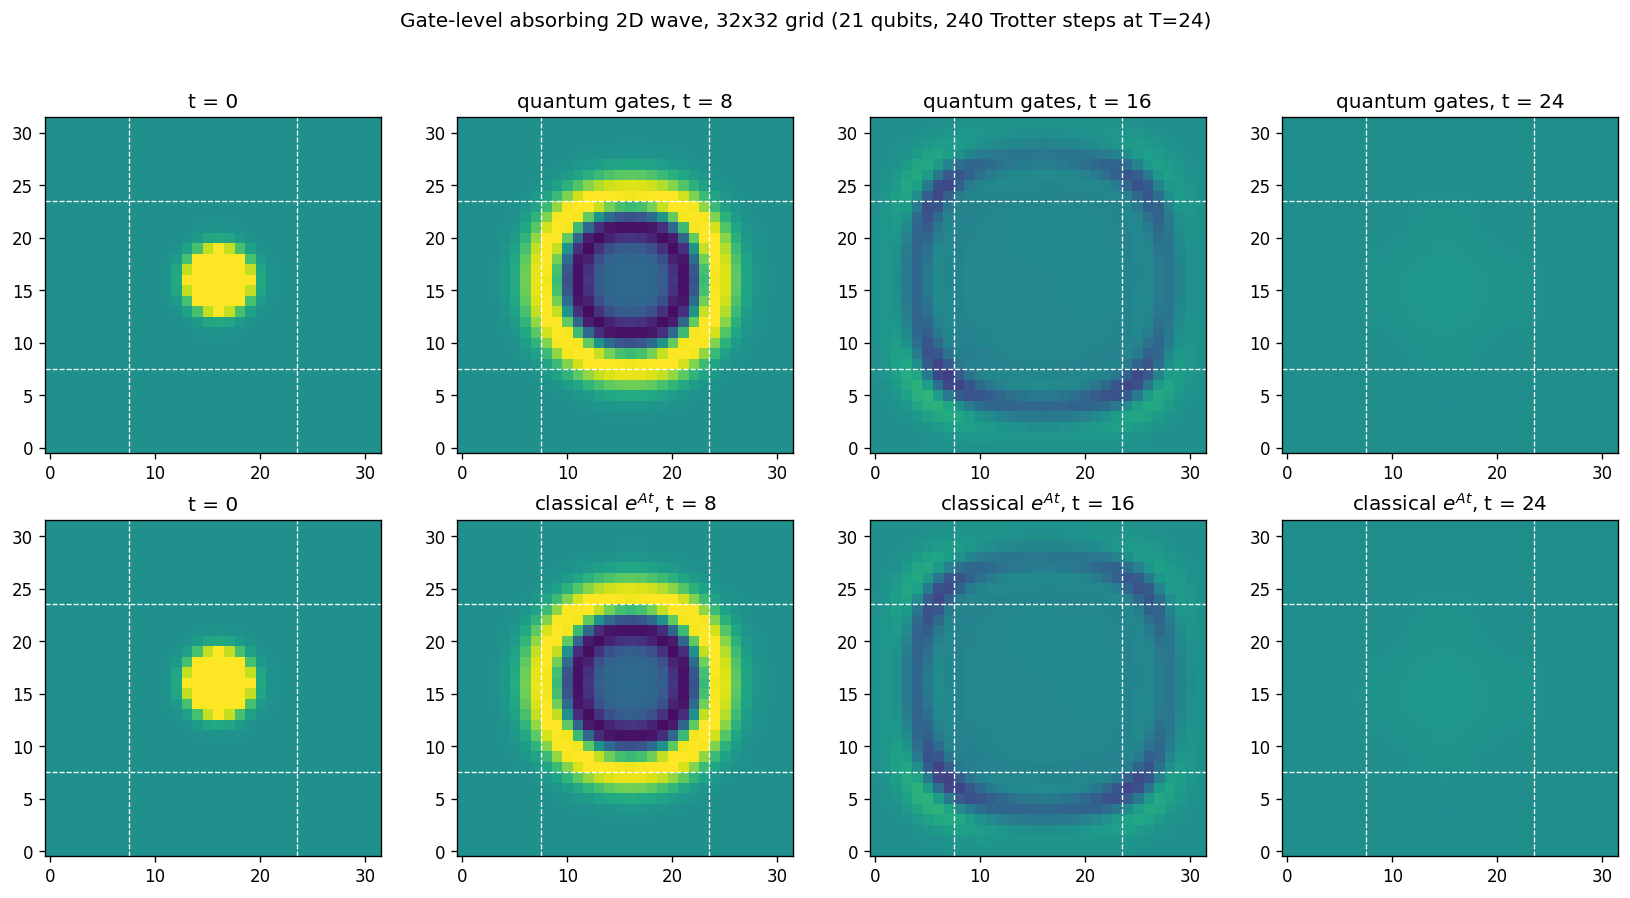
\includegraphics[width=\linewidth]{chapter3/fig6_2d_gate_level_32x32.png}
  \caption{Gate-level absorbing 2D wave evolution at scale: $32\times32$
  grid, 21 qubits (12 system $+$ 9 $p$-register), up to 240 second-order
  Trotter steps (983 native operations per step).  Top row: recovered
  field from the quantum circuit at $t=0,8,16,24$ (dashed lines mark the
  absorbing-layer strips).  Bottom row: exact reference $e^{At}\psi_0$.
  The outgoing ring is absorbed across the layer; the total energy decays
  from $0.97$ to $1.25\times10^{-3}$, and the recovered field matches the
  reference to $7.7\times10^{-3}$--$1.7\times10^{-2}$.}
  \label{ch3:fig:gate21}
\end{figure}

% ======================================================================
\subsection{Complexity}
\label{ch3:sec:complexity}

Term counts inherit the QTT structure of the difference operators:
$2n_x+2$ terms in 1D and $4n_x+4$ in 2D ($n_x=n_y$), exactly linear in
the register size (fitted slopes $4.000/2.000$, intercepts $4/2$).
Transpiled to the $\{\mathrm{CX},u\}$ basis, one Strang wave step costs
$217/459/834/1343$ operations for $n_{\mathrm{sys}}=6/8/10/12$; a
power-law fit gives exponent $2.63$ with $r^{2}=0.99997$
(\ref{ch3:fig:gatecounts})---convincingly polynomial, and in fact
asymptotically quadratic: the term count is linear in $n$ and the
ancilla-free V-chain multi-controlled-$R_z$ is linear in its control
count, so ops/step $=O(n^{2})$.  The constants are fixed by the
measurements.  The per-step cost in the
$\{\textsc{cx}, U\}$ basis is reproduced to $0.03\%$
($r^{2}=0.9999999$) by the quadratic
\begin{equation}
  G_{\mathrm{step}}(n) \;=\; 16.7\,n^{2} - 112.7\,n + 293,
  \label{ch3:eq:stepcost}
\end{equation}
whose structure is transparent: a Strang step exponentiates $2n$
Hermitian-paired terms ($4n_x+4$ at $n=2n_x+2$), each one Bell basis
change plus one multi-controlled $R_z$ whose ancilla-free V-chain cost
is \emph{exactly} $32k-31$ elementary operations for $k\ge8$ controls
(measured), linear in $k$; with the QTT ladder structure averaging
$\bar k\approx n/4$ controls per term, the leading coefficient is
$2n\cdot32\,\bar k/n^{2}\approx16.7$.  The total gate count is steps
$\times$ ops/step with steps $= T/\delta t$ and $\delta t$ set by the
second-order bound $\delta t = \sqrt{\varepsilon_{\mathrm{tr}}/(C_2
T)}$, where $C_2$ is the Strang error constant of the slope-$(-2)$ fits
of \ref{ch3:fig:convergence}(d):
\begin{equation}
  G_{\mathrm{total}}
  \;=\; \sqrt{\frac{C_2\,T^{3}}{\varepsilon_{\mathrm{tr}}}}\;
        G_{\mathrm{step}}(n)
  \;=\; O\!\left(\frac{T^{3/2}}{\sqrt{\varepsilon_{\mathrm{tr}}}}\;
        n^{2}\right),
  \label{ch3:eq:totalcost}
\end{equation}
plus the damping diagonal per step and two $\mathrm{QFT}(n_p)$; the
power-law fit across the measured range reads $n^{2.63}$ because the
subleading terms of Eq.~\eqref{ch3:eq:stepcost} have not yet decayed at
$n\le12$.

\emph{Caveat (honest).}  The damping factor is a single native
\texttt{diagonal} instruction on the simulator, but a \emph{generic}
diagonal on $n$ qubits synthesises to $\Theta(2^{n})$ elementary gates:
we measure a CX count of exactly $2^{n}-2$ and totals within 15\% of the
$2^{n+1}-3$ synthesis bound.  For hardware the structure must be
exploited: the diagonal is $D_\eta\otimes\Sigma$ with $\eta$ linear in
the $p$ index and $\sigma$ a degree-$m$ polynomial profile on the layer
strips, so phase-polynomial constructions give $\mathrm{poly}(n)$
circuits, and the logic-minimisation synthesis of piecewise-constant
diagonal operators of Ref.~\cite{sato2025nonconservative}
(Espresso-compressed projector strings with matrix-product-state
coefficient oracles) provides an existing $\mathrm{poly}(n)$ toolbox
directly applicable to the strip-wise polynomial $\sigma$ profiles;
making this explicit is deferred to future work.

\begin{figure}
  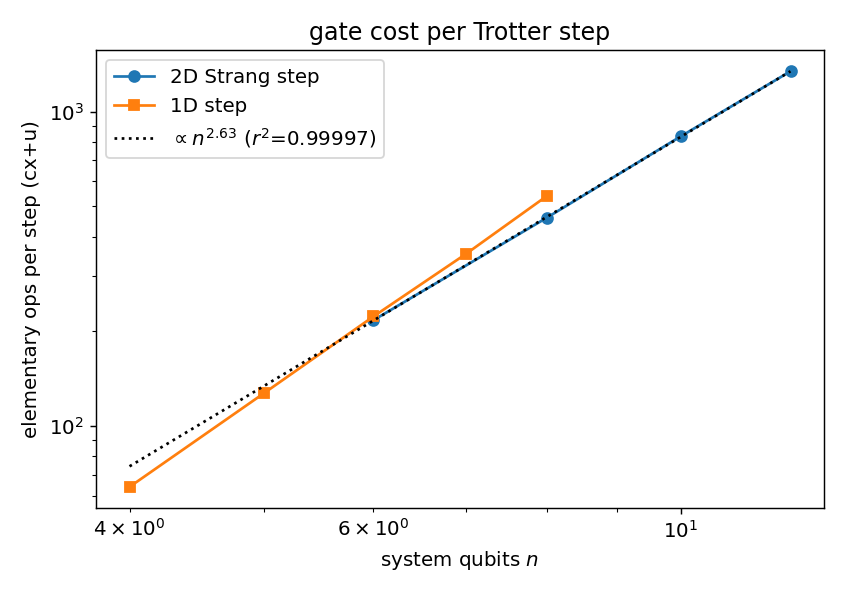
\includegraphics[width=\linewidth]{chapter3/paper_P3_gatecounts.png}
  \caption{Gate cost per Trotter step after transpilation to the
  $\{\mathrm{CX},u\}$ basis, versus the number of system qubits $n$: 1D
  steps (squares) and 2D Strang steps (circles).  The dotted line is the
  power-law fit $\propto n^{2.63}$ ($r^{2}=0.99997$) to the 2D series;
  the term count itself is exactly linear in $n$ (Section~\protect\ref{ch3:sec:complexity}).}
  \label{ch3:fig:gatecounts}
\end{figure}

% ======================================================================
\subsection{Discussion and outlook}
\label{ch3:sec:discussion}

The $\lambda^{+}$ obstruction of Lemma~\ref{ch3:lem:threshold} is generic for
auxiliary-field absorbers---memory variables, auxiliary-differential-equation
formulations, split fields---because the injection/source asymmetry is
structural rather than an artefact of one discretisation.  The Lyapunov
symmetrizer is the corresponding general remedy, and its
quantum-implementable variants (block-encoding $S$, structured or banded
approximate symmetrizers) are open.  Natural next steps include a
hardware experiment in the style of Ref.~\cite{sato2024hamiltonian};
quantum-signal-processing or qubitisation in place of Trotter (and the
query-optimal Schr\"odingerisation formulation of
Ref.~\cite{jin2025queries}); CPML for Maxwell's equations
\cite{jin2023maxwell,ma2024maxwellcircuits}; and smoother warping
profiles (error-function or numerically optimal) beyond the $C^{1}$ cubic.

\medskip
\noindent\emph{Code and data availability.}  The implementation
(\texttt{lib/absorbing.py}, \texttt{lib/schrodingerisation.py}), all
experiment scripts and JSON result files
(\texttt{paper/experiments/}), and the executed demonstration notebook
are available in the accompanying repository at
\url{https://github.com/x-repos/qawave-cpml}.

% ======================================================================


\subsection{Proof of Lemma~\protect\ref{ch3:lem:threshold}}
\label{ch3:app:proof}

Fix a layer node $j$ with $\sigma_j>0$ and a stencil neighbour $i$ such
that the difference entry satisfies $|D_{ji}|=1/h$ (wave speed $c=1$;
the general case restores a factor $c$ in Eq.~\eqref{ch3:eq:lemmarate}).
Write $\beta=\sigma_j/\kappa_j+\alpha_j\ge0$ for the CFS decay rate,
$\gamma$ for the injection coefficient, and
$s=\sigma_j|D_{ji}|/(\kappa_j^{2}\gamma)$ for the memory-source
magnitude.  Let $G=\diag(g)>0$ be \emph{any} positive diagonal
similarity, and set
\begin{equation}
  u=\frac{g_{v_j}}{g_{\phi_j}}, \qquad
  t=\frac{g_{\phi_j}}{g_{w_i}}, \qquad
  \rho=u\,t=\frac{g_{v_j}}{g_{w_i}}.
  \label{ch3:eq:scalings}
\end{equation}
The transformed generator $\At = GAG^{-1}$ has unchanged diagonal, and
the three relevant coupling families scale as follows.
\begin{enumerate}
\item[(i)] \emph{Injection pair} $(v_j,\phi_j)$: entry $u\gamma$, reverse
  entry $0$, so $\Ht$ contains the principal $2\times2$ submatrix
  \begin{equation}
    \begin{bmatrix} 0 & u\gamma/2 \\ \bar u\bar\gamma/2 & -\beta
    \end{bmatrix}
    \;\Longrightarrow\;
    \lamax(\Ht) \ge f(|u|\gamma,\beta),
  \end{equation}
  with $f(x,\beta):=\bigl(\sqrt{\beta^{2}+x^{2}}-\beta\bigr)/2$.
\item[(ii)] \emph{Memory-source pair} $(w_i,\phi_j)$: entry $t\,s$
  analogously, giving $\lamax(\Ht)\ge f(|t|s,\beta)$.
\item[(iii)] \emph{Physical wave pair} $(v_j,w_i)$: elementwise,
  $\At[v,w]=-iD_{ji}\,\rho$ and $\At[w,v]=+iD_{ji}/\rho$ (using that $D$
  is real and $D^{\dagger}=-D_{\mathrm{b}}$), so
  \begin{equation}
  \begin{split}
    \Ht[v_j,w_i] &= \frac{iD_{ji}}{2}\bigl(\rho^{-1}-\rho\bigr) \\
    \Longrightarrow\quad
    \lamax(\Ht) &\ge \frac{|D_{ji}|}{2}\,\bigl|\rho^{-1}-\rho\bigr|.
  \end{split}
  \end{equation}
\end{enumerate}
All three are lower bounds on $\lamax(\Ht)$ by Cauchy interlacing (the
eigenvalues of any principal submatrix interlace those of the full
Hermitian matrix).

\emph{Case analysis.}  If $|\rho|\le1/2$ then
$|\rho^{-1}-\rho|\ge3/2$, so (iii) gives $\lamax(\Ht)\ge3/(4h)$.
Otherwise $|\rho|>1/2$ implies
\begin{equation}
  |u\gamma|\cdot|t\,s| \;=\; |\rho|\,\gamma s \;>\; \frac{\gamma s}{2}
  \;=\; \frac{\sigma_j|D_{ji}|}{2\kappa_j^{2}},
\end{equation}
hence
$\max(|u|\gamma,\,|t|s)\ge\sqrt{\sigma_j/(2h\kappa_j^{2})}$ and
(i)--(ii) give
$\lamax(\Ht)\ge f\bigl(\sqrt{\sigma_j/(2h\kappa_j^{2})},\,\beta\bigr)$.
Therefore, for every positive diagonal scaling,
\begin{equation}
  \lamax(\Ht) \;\ge\; \min\left\{\frac{3}{4h},\;
  \frac{\sqrt{\beta^{2}+\sigma_j/(2h\kappa_j^{2})}-\beta}{2}\right\},
  \label{ch3:eq:appbound}
\end{equation}
which is $\Theta\bigl(\sqrt{\sigma_j/h}\bigr)$ as $h\to0$ (the second
branch is the minimum once $\sigma_j/(2h)\gg\beta^{2}$, i.e.\ for any
fixed profile and small $h$).  The bound is independent of $\gamma$ and
of the scaling $G$.  The explicit balanced choice
$\gamma^{*}=\sqrt{2\sigma_{\max}/h}$ attains the same rate from above:
measured $\lambda^{+}=0.68$--$0.97$ across our configurations, versus the
lower bound $0.18$ at the $8\times8$, $\sigma_{\max}=0.5$ parameters---the
bound is a rate, not a sharp constant. \hfill$\blacksquare$

\medskip
\emph{Consistency check.}  The collapsed 1D form
(Section~\ref{ch3:sec:1d}) has no injection pair: the memory is eliminated and
the damping is diagonal, so the lemma does not apply---and indeed
$H_1=-\diag(\sigma)\preceq0$ there.

\chapter{Seismic Traveltime Inversion with Quantum Annealing}\label{chap:seismic-qa}

\begin{center}
    A paper published in \emph{Scientific Reports}\footnote{Nguyen, H. A. and Tura, A. Seismic traveltime inversion with quantum annealing. \emph{Scientific Reports}, 15, 17984 (2025). \href{https://doi.org/10.1038/s41598-025-01188-8}{https://doi.org/10.1038/s41598-025-01188-8}}.

    Hoang Anh Nguyen\footnote{Department of Geophysics, Colorado School of Mines, Golden, Colorado 80401, USA\label{note:ch3-mines}}$^,$\footnote{Primary researcher and author for correspondence}
    and Ali Tura$^{\ref{note:ch3-mines}}$
\end{center}

\subsection{Abstract}

This study demonstrates the application of quantum computing based quantum annealing to seismic traveltime inversion, a critical approach for inverting highly accurate velocity models. The seismic inversion problem is first converted into a Quadratic Unconstrained Binary Optimization problem, which the quantum annealer is specifically designed to solve. We then solve the problem via quantum annealing method. The inversion is applied on a synthetic velocity model, presenting a carbon storage scenario at depths of 1000-1300 meters. As an application example, we also show the capacity of quantum computing to handle complex, noisy data environments. This work highlights the emerging potential of quantum computing in geophysical applications, providing a foundation for future developments in high-precision seismic imaging.

\subsection{Introduction}

Quantum computing is an emerging field with significant promise for various scientific and engineering disciplines. As we stand at the frontier of this technological revolution, early-stage research in quantum computing is crucial for the advancement of geophysics. Numerous studies have begun to explore the integration of quantum computing within this field, highlighting its immense and revolutionary potential \cite{moradi18}. For instance, quantum annealers can perform well in solving tomography optimization problems \cite{sarkar18}.  The quantum computing is applied for binary-value full waveform inversion, addressing issues related to velocity variations \cite{greer20}. In the frequency domain, the seismic wave equation can be reduced to a system of linear equations, allowing for the application of quantum annealing \cite{kumar22}. Furthermore, it has been shown that quantum annealing impedance inversion with L1 norm regularization can dramatically enhance accuracy and anti-noise capabilities \cite{wang24}.

A quantum annealer is a specific type of quantum computer designed to solve optimization problems \cite{Yulianti22}.
The quantum annealing process in quantum annealers can find the minimum energy state of a system, corresponding to the optimal solution of a given problem \cite{MCGEOCH20}. This process is achieved by utilizing quantum fluctuations, allowing the system to tunnel through energy barriers \cite{crosson16}. While there are various types of models in quantum computing \cite{nimbe21,Lu2023}, this particular feature allows quantum annealing to efficiently explore complex energy landscapes, making them particularly well-suited for solving optimization problems.

Most previous attempts to address seismic problems using quantum annealers have primarily involved relatively simple models \cite{Alulaiw15, Albino22}. For conventional approach by classical computers, the cross-well seismic inversion between boreholes can be computationally expensive \cite{mcmechan83}, necessitating the development of new methods to tackle these challenges. Therefore, in this study, we aim to advance this line of research by applying quantum annealing to a complex problem: Seismic traveltime inversion of the velocity model between two boreholes. Our focus is on developing an inversion strategy that can accurately invert the velocity model with noisy data despite the limitation of the quantum hardware, specifically targeting carbon storage scenarios at depths of 1000-1300 meters. We use quantum annealer at D-Wave Advantage System, which has at least 5000 qubits \cite{mcgeoch2020d}. Clearly, this travel-time inversion method can be applied to other acquisition geometries and data such as surface seismic, vertical seismic profile (VSP), earthquake or micro seismic data.

\subsection{Results}

We start the quantum annealing inversion process with exact traveltime data without noise and constant initial velocity model \(v_{ini}\) of 3475 m/s. The initial model and the results of the inverted model \(v_{inv}\) at each iteration obtained after the first 9 iterations indicate rapid convergence (\ref{fig:ch3-result10loops}). Notably, in the first iteration, the carbon storage area is immediately identified with high precision.

\begin{figure}[!ht]
\centering
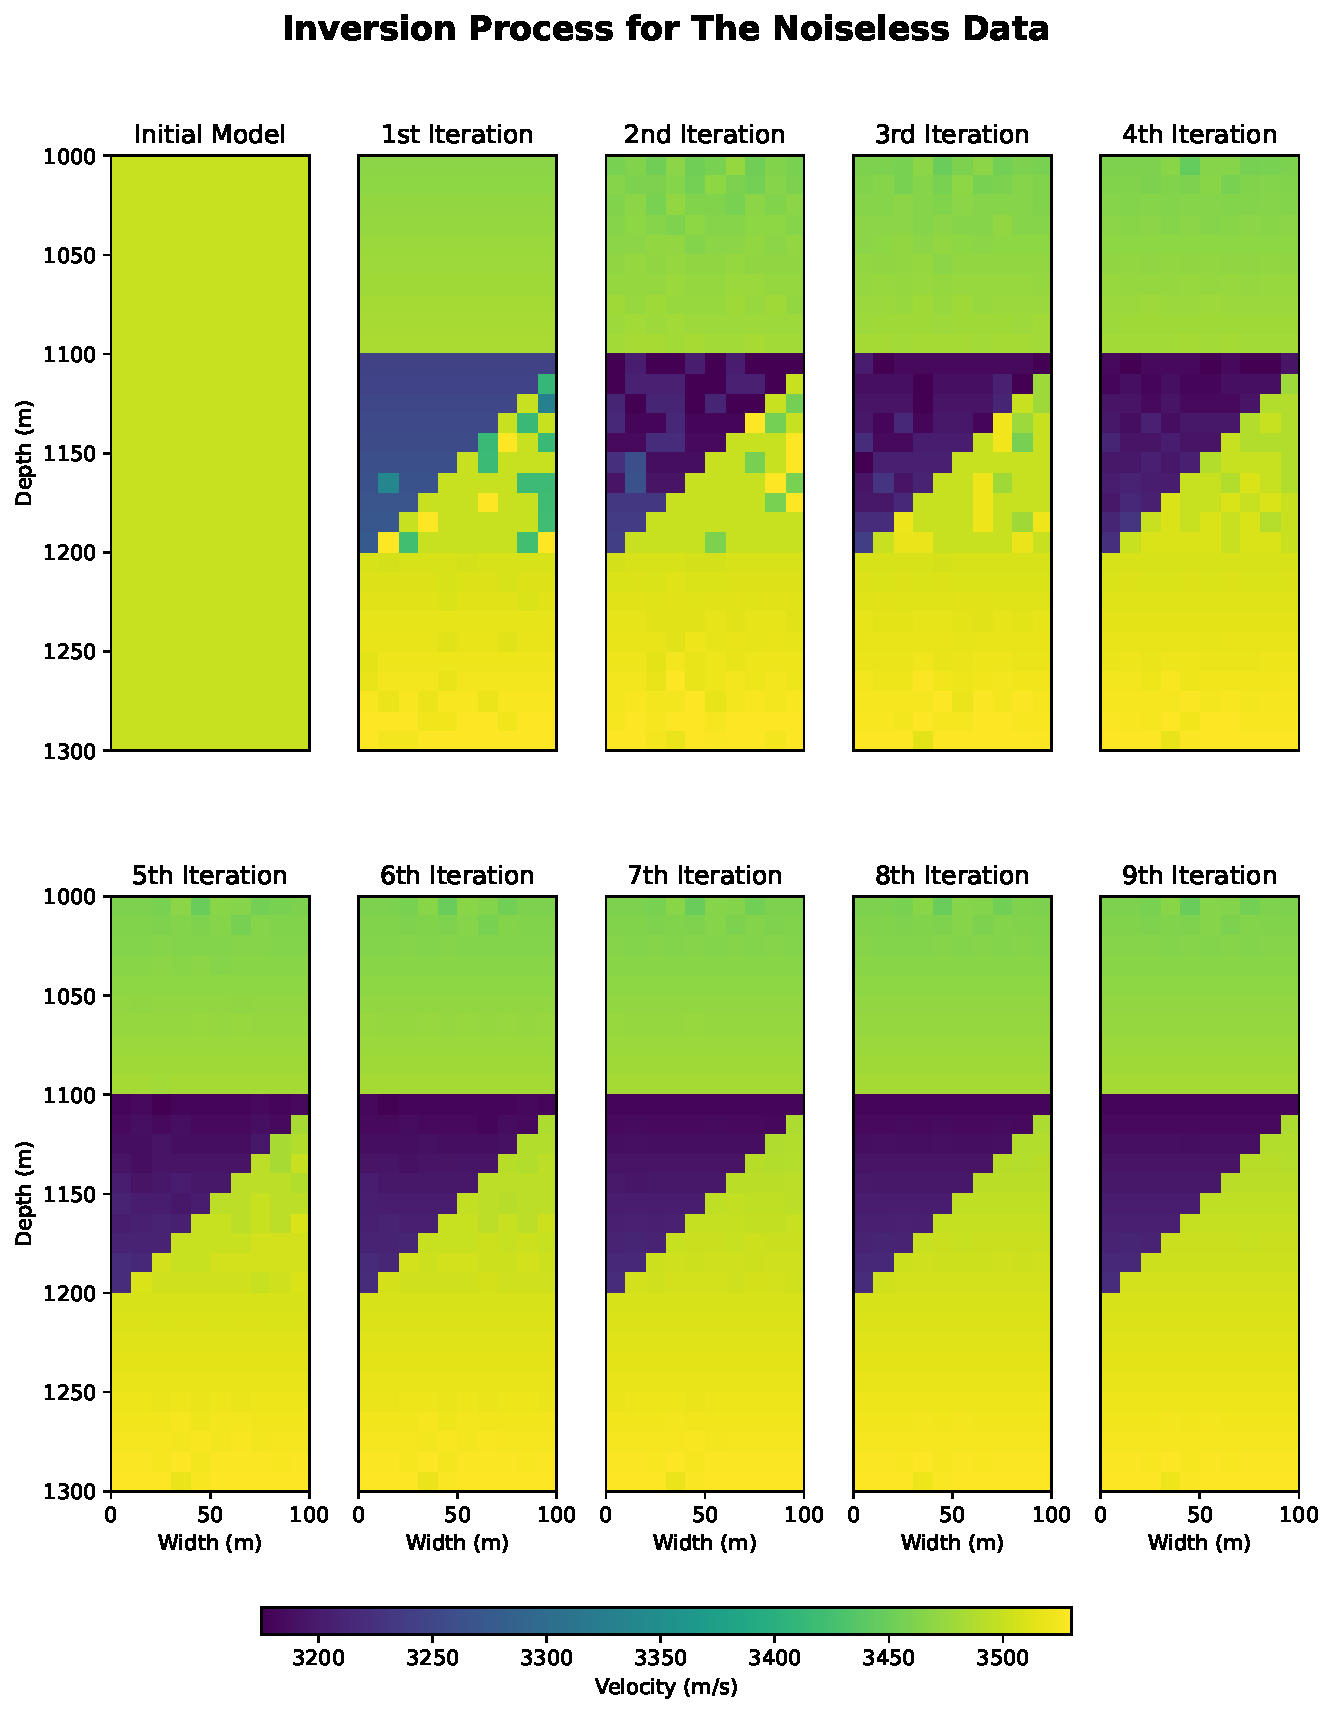
\includegraphics[width=0.9\linewidth]{chapter4/result10loops.pdf}
\caption{The starting model \(v_{ini}\) and the inverted velocity model \(v_{inv}\) over the first 9 iterations with exact, noise-free traveltime data.}
\label{fig:ch3-result10loops}
\end{figure}

The component-wise relative errors \({e}_{ij}\) between the true \(v_{true, ij}\) and final inverted velocity model \(v_{final, ij}\) after 10 iterations is shown in \ref{fig:ch3-result-diff}. The component-wise relative errors are calculated by \({e}_{ij} = |v_{inv, ij} - v_{true, ij}| / |v_{true, ij}|\). The most significant errors occurs in the shallow and deep regions with weakest constraints, yielding a maximum relative error value of about 0.326\%. In contrast, the carbon storage area, spanning depths from 1100 to 1200 m, demonstrates exceptionally low errors due to the high ray coverage. The high-accuracy result underscores the effectiveness of the quantum annealing approach to the traveltime inversion.

\begin{figure}[!ht]
\centering
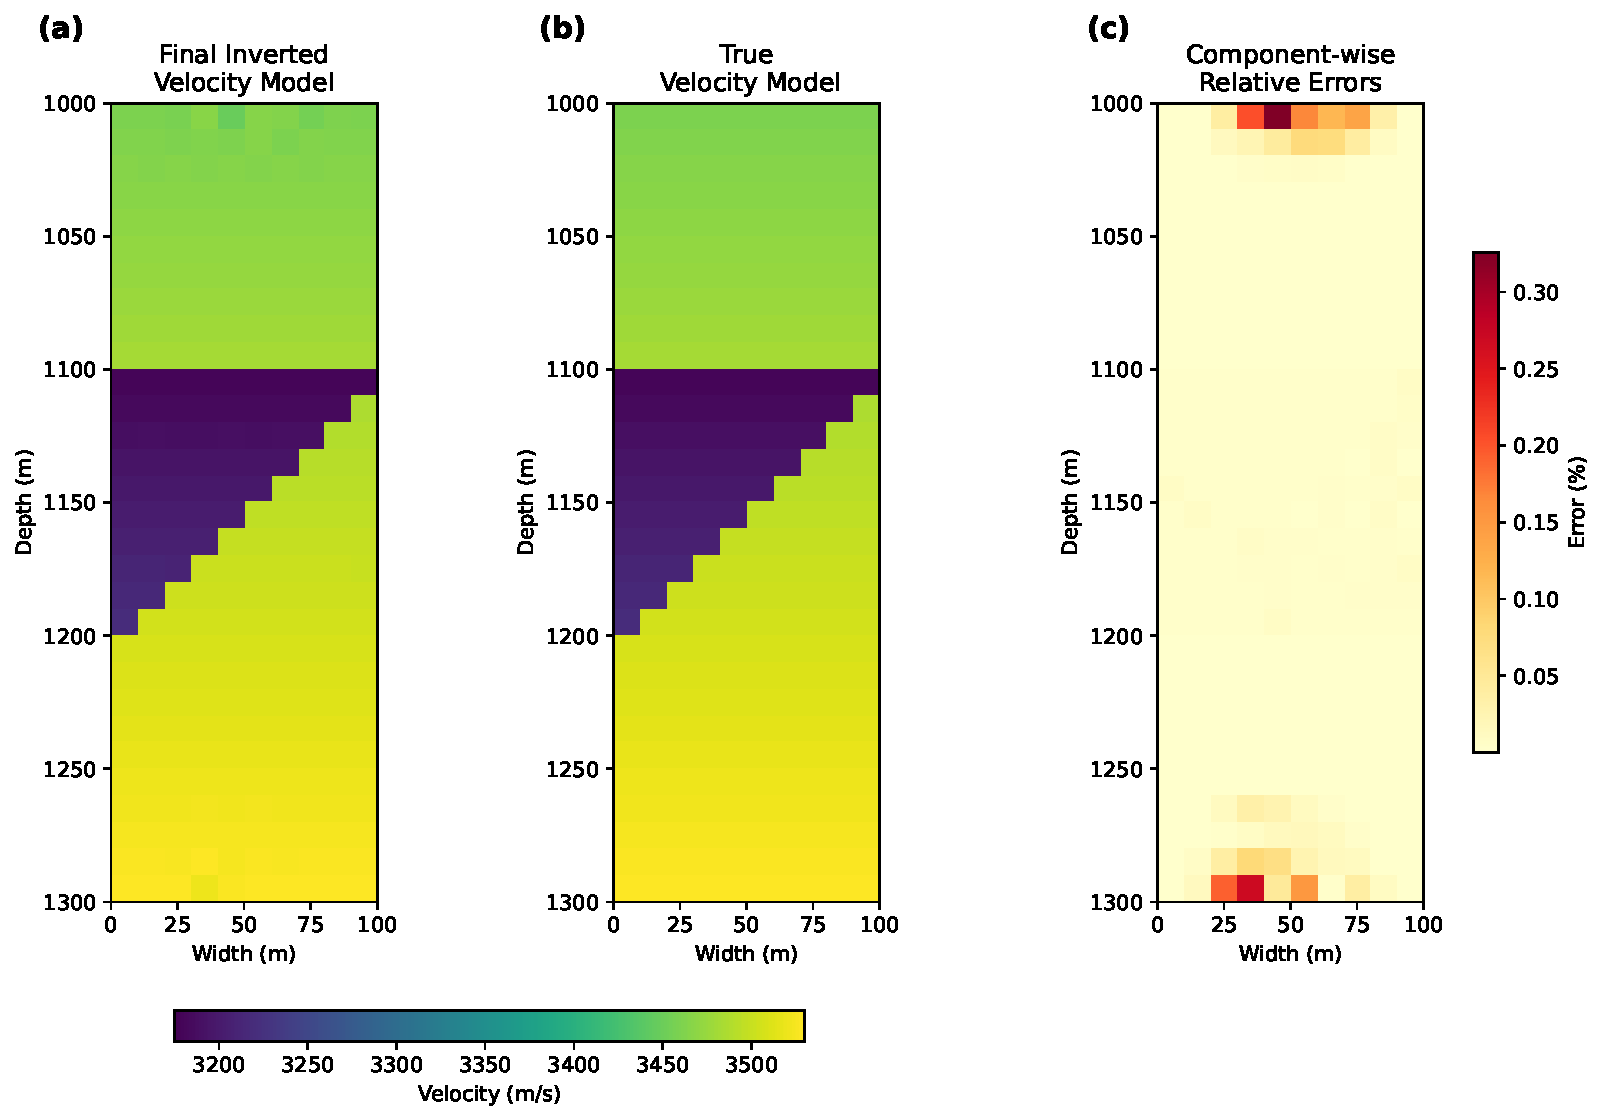
\includegraphics[width=0.9\linewidth]{chapter4/result_diff.pdf}
\caption{Velocity models and error: (a) final noiseless inverted model after 10 iterations \(v_{inv, ij}\), (b) true model \(v_{true, ij}\), and (c) the component-wise relative errors \(e_{ij}\) between the final inverted and true velocity model.}
\label{fig:ch3-result-diff}
\end{figure}

For seismic traveltime inversion problem, the quantum annealing method and the classical linear least squares approach produce similar levels of error under ideal conditions, where data is free of noise \cite{Souza22}. However, real-world data often contain random noise, making it essential to assess the robustness of these methods under realistic conditions. Since we use the first-arrival traveltime, the data is relatively clean \cite{Daley2008}. Therefore, we introduce the random noise in a range from 1\% to 5\% into the synthetic data. We compare the outcomes of the Tikhonov regularization least squares, serving as the standard method, with that of the quantum annealing method.

\begin{figure}[!ht]
\centering
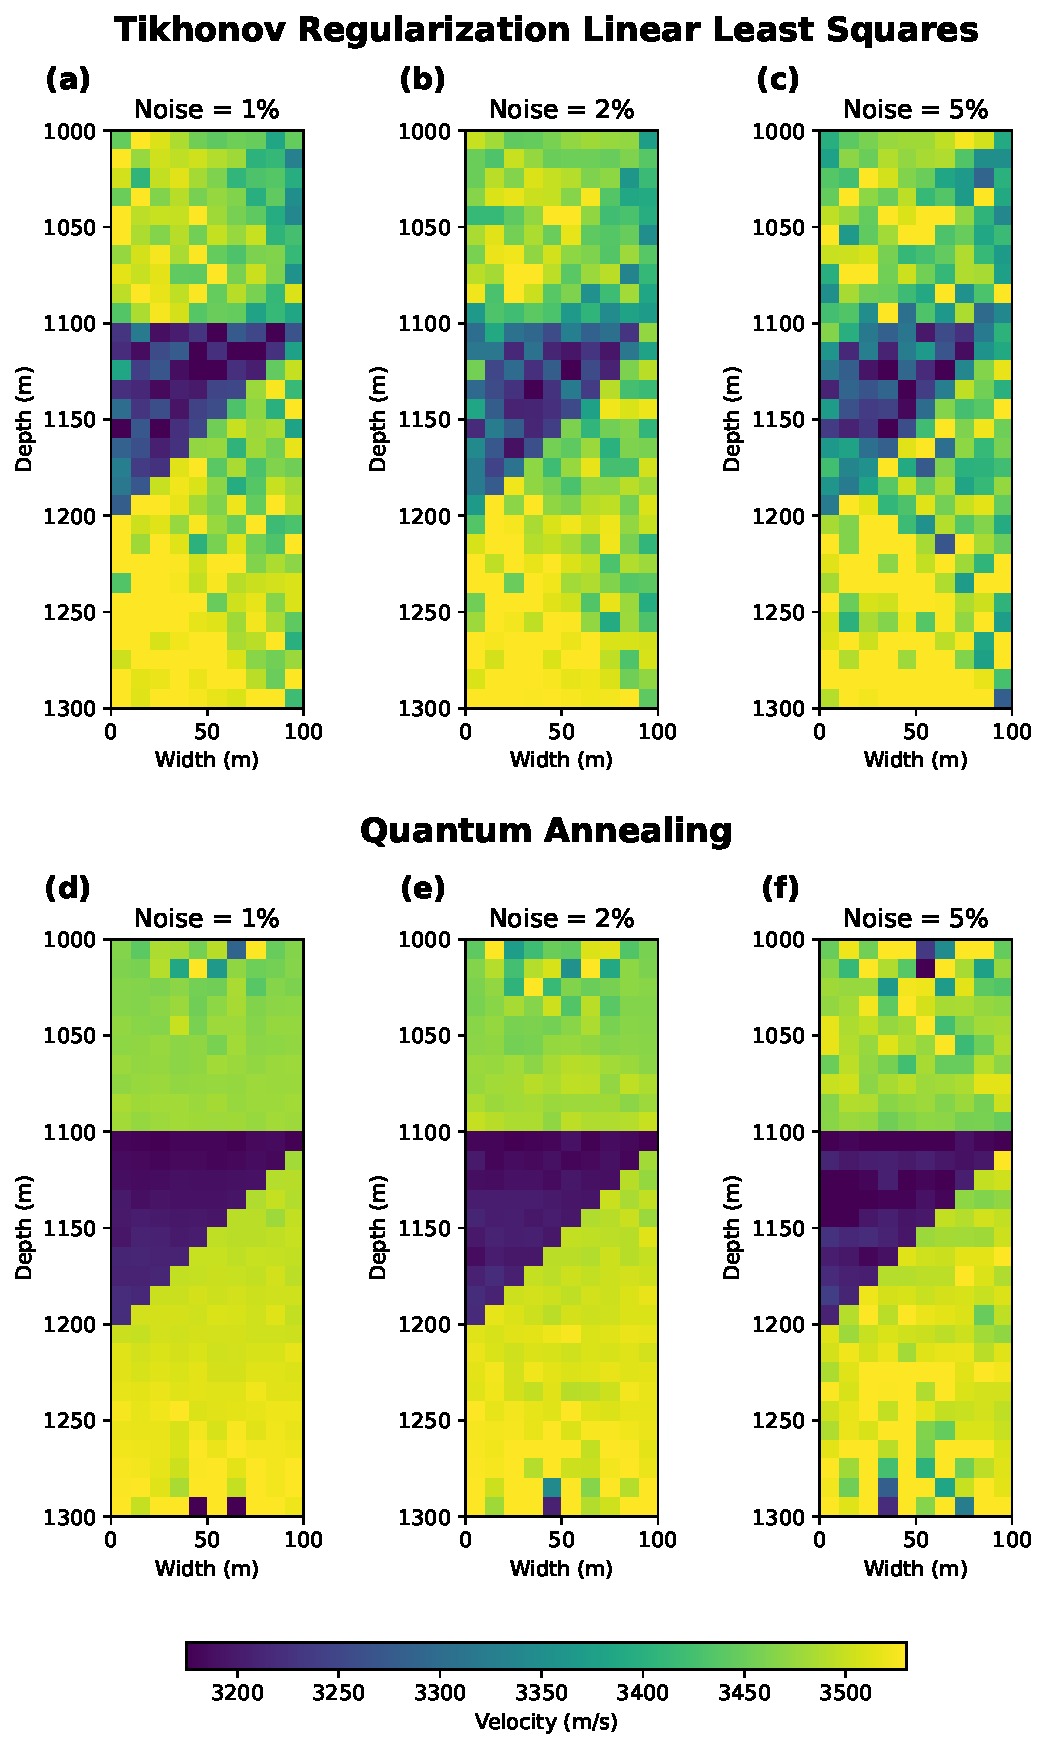
\includegraphics[width=0.7\linewidth]{chapter4/combined_velocity_inversions.pdf}
\caption{Traveltime inversion results with different noisy data using linear least squares (a, b, c) and quantum annealing method (d, e, f)}
\label{fig:ch3-noise-comparison}
\end{figure}

The results reveal a stark contrast in the sensitivity of these methods to noise. In this problem, the Tikhonov regularization linear least squares method is sensitive to noise (\ref{fig:ch3-noise-comparison}a, b, c). At the noise level of 1\% of the traveltime, while this method can identify the region of carbon storage, the deviation of the inverted model from true model is considerable. As the noise level increases to  2\% and 5\% of the traveltime, the linear least squares method almost fails to accurately determine the velocity model. This significant sensitivity limits its effectiveness in processing noisy seismic data, posing challenges for practical applications.
In contrast, with the same noise, the quantum annealing method is more robust (\ref{fig:ch3-noise-comparison}d, e, f). At the 1\% noise level, the differences between the noise-free model and the results obtained are small. Differences start to appear primarily in shallow and deep areas where there is less constraint. Remarkably, at the 5\% noise level, the quantum annealing method still effectively reproduces the velocity model. In areas with high ray coverage, these differences are small. This analysis underscores the potential of quantum annealing method for handling noisy seismic data more effectively than the classical linear least squares method.

\subsection{Discussion}

In this study, we demonstrate several advancements to enhance the robustness and accuracy of seismic traveltime inversion results using the quantum annealing method. A significant improvement involves incorporating non-uniform source and receiver spacing. By using non-uniform spacing, we achieve better ray coverage of both shallow and deep regions, thereby increasing the overall accuracy of the final inverted velocity model.

The initial problem is broken down into smaller sub-problems, we also introduce the boundary \(L\) during the inversion process for better constraint and accommodating hardware limitations. While this paper does not utilize parallel processing, solving these sub-problems independently enables parallel execution, which can significantly reduce computational time.

For practical applications where noise is an unavoidable factor, our method demonstrates a remarkable ability to handle noisy data effectively and is highly suitable for the ill-conditioned problems, maintaining high efficiency and accuracy. The key advantage of the quantum annealing method is its ability to locate the global minimum of the objective function more effectively than classical methods, which are often trapped in local minima. Quantum tunneling allows the quantum system to explore a broader solution space and tunnel barriers that would hinder classical optimization methods \cite{Finnila94}. This method can result in more accurate and reliable inversion outcomes, particularly in complex and heterogeneous environments. The quantum annealer solves problems using principles of quantum mechanics, which inherently depend on the operating environment of the machine. Consequently, running the same problem multiple times may yield slightly different results because of the probabilistic nature of quantum computations \cite{Delgado11, Hevia21}. However, we expect the advancements in quantum technology will decrease this variability and also reduce computational time.

\subsection{Conclusion}

The integration of quantum annealing in seismic traveltime inversion represents a potentially major advancement in geophysics. We utilise the open-access D-Wave Advantage quantum annealer to solve the inversion problem for a synthetic velocity model, representing a carbon storage scenario.
The quantum annealing recursive method can give a good inverted velocity result after 10 iterations. Notably, the quantum method outperforms the classical linear least squares method in dealing with noisy data, where classical methods sometimes struggle. Despite promising results, the current state of quantum computing is not without its challenges. The slight variability in the results due to quantum noise \cite{Li_2020, Franca2021, Leon21} requires multiple runs to ensure reliable results. However, these challenges are expected to diminish as advances in quantum technology continue. This study suggests that quantum annealing could revolutionize seismic inversion processes, offering more accurate solutions in scenarios where traditional methods are computationally intensive or even infeasible. As quantum computing matures, its applications in geophysics are likely to expand, encompassing more complex and larger-scale problems. This research not only underscores the potential of quantum annealing in seismic inversion but also sets the stage for future exploration into other areas of inverse problems. We expect that continued development of quantum computing technologies promises to unlock new capabilities, possibly making it an indispensable tool for new challenges.

\subsection{Methods}

\subsubsection{Quantum Annealing}

Quantum computing is rapidly emerging as a pivotal area of scientific and technological advancement, attracting considerable investment and interest due to its profound potential \cite{britt17, moller17, coccia24}. Unlike classical computers that use bits, which exist only in states of 0 or 1, quantum computers employ quantum bits, or qubits. Qubits possess unique properties such as superposition, entanglement, and interference \cite{qiao18, neeley10, loft20}, enabling them to perform certain complex computations beyond the capabilities of classical computers \cite{Feld19, Neukart17}. Qubits can be constructed from various physical systems such as photons, trapped atoms, nuclear magnetic resonance, quantum dots, dopants in solids, and superconductors \cite{ladd10}. Previous research \cite{baldassi18, Denchev16,albash18, Nakata2014, Senekane21} has provided evidence that quantum computing possibly surpasses classical computers in terms of processing speed and efficiency for certain problems.

The quantum annealing process facilitates the finding of the global minimum of a cost function efficiently. This process can be described using the real-time Schr\"odinger equation \cite{morita08}:
\begin{equation}
i \hbar \frac{d}{dt} |\Psi(t)\rangle = H(t)|\Psi(t)\rangle
\label{eq:ch3-schrodinger}
\end{equation}
where \(| \cdot \rangle \)  is the ket of the Dirac notation \cite{Dirac_1939}, \(i\) is the imaginary unit, \( t \) is time, \( \hbar\) is the reduced Planck's constant, \( \Psi(t) \) is the wave function, \(|\Psi(t)\rangle \) is the quantum state vector, \( H \) is the Hamiltonian representing the total energy of the quantum system \cite{Griffiths_Schroeter_2018, Shankar1994}. If \(\hbar\) is set as 1, \Eqref{eq:ch3-schrodinger} becomes:
\begin{equation}
i \frac{d}{dt} |\Psi(t)\rangle = H(t)|\Psi(t)\rangle
\label{eq:ch3-schrodinger-hbar1}
\end{equation}

The Hamiltonian in quantum annealing can be composed of two components \cite{rajak23, biswas17}:
\begin{equation}
H(t) = A(t) H_0 + B(t) H_1
\end{equation}
where \( H_0 \) is the initial Hamiltonian, representing a system with an initial ground state. \( H_1 \) is the final Hamiltonian, whose ground state encodes the solution to the optimization problem. \( A(t) \) and \( B(t) \) are time-dependent coefficients. \( A(t) \) and \( B(t) \) are set in a range of 0 to 1 so that \( A(t_0) \gg B(t_0) \) at the initial time \( t_0 \) and \( B(t_1) \gg A(t_1) \) at the final time \( t_0 \). During the process, \( A(t) \) monotonically decreases, while \( B(t) \) monotonically increases. At the start of the annealing process, \( H(t) \approx H_0 \). At the end of the annealing process, \( H(t) \approx H_1 \). Thus, the system transitions from the ground state of \( H_0 \) to the ground state of \( H_1 \). If \( H(t) \) changes sufficiently slowly, the state evolves adiabatically \cite{hauke20}.

The problems are then often mapped onto a Quadratic Unconstrained Binary Optimization (QUBO) or Ising model \cite{willsch22}:
\begin{equation}
\text{QUBO:} \quad \min_{x_j = 0,1} \left( \sum_{j \leq k} x_j Q_{jk} x_k + C_1 \right)
\label{eq:ch3-qubo}
\end{equation}
\begin{equation}
\text{Ising:} \quad \min_{s_j = \pm1} \left( \sum_j h_j s_j + \sum_{j < k} J_{jk} s_j s_k + C_2 \right)
\label{eq:ch3-ising}
\end{equation}
where \(j, k\) are indices, ranging over all qubits. In the QUBO model (\Eqref{eq:ch3-qubo}), \(Q_{jk}\) is the QUBO matrix with values \(Q_{jk} \in \mathbb{R}\). The binary variable vector is \(\mathbf{x}\) with \(x_j \in \{0, 1\}\). In the Ising model (\Eqref{eq:ch3-ising}), the problem is defined by the biases \(h_j \in \mathbb{R}\) and the couplers \(J_{jk} \in \mathbb{R}\), and the binary variable vector is \(\mathbf{s}\) with \(s_j \in \{-1, 1\}\). \(C_1\) and \(C_2\) are constants which do not affect the solution of the optimization problem. The Ising model and the QUBO model are mathematically equivalent, allowing them to be translated into each other. This equivalence provides a flexible approach to problem-solving, enabling the conversion of problems between these models based on the requirements and available tools. There are also tools, such as \texttt{ToQUBO.jl}, designed to convert standard problems into the QUBO format \cite{toqubo23}. In this paper, we utilize the quantum annealer from D-Wave Advantage Systems \cite{mcgeoch2020d} to employ direct quantum processing unit (QPU) methods for seismic travel inversion.

\subsubsection{Seismic Data Acquisition}

We construct a velocity model representing carbon storage applications, as shown in \ref{fig:ch3-ray-coverage}a. This model spans a depth range from 1000 m to 1300 m and extends 100 m horizontally. The size of the grid cell for this model is 10 x 10 m. Within this model, the carbon storage structure is depicted as a wedge, starting from 1100 m and reaching a maximum depth of 1200 m. The velocity model is constructed with varying velocities to reflect real-world geological conditions. The average velocity within the carbon storage area ranges from 3180 to 3220 m/s, which is about 11\% lower than the surrounding background velocity, which ranges from 3530 to 3640 m/s. Furthermore, the velocities increase with depth.

\begin{figure}[!ht]
    \centering
    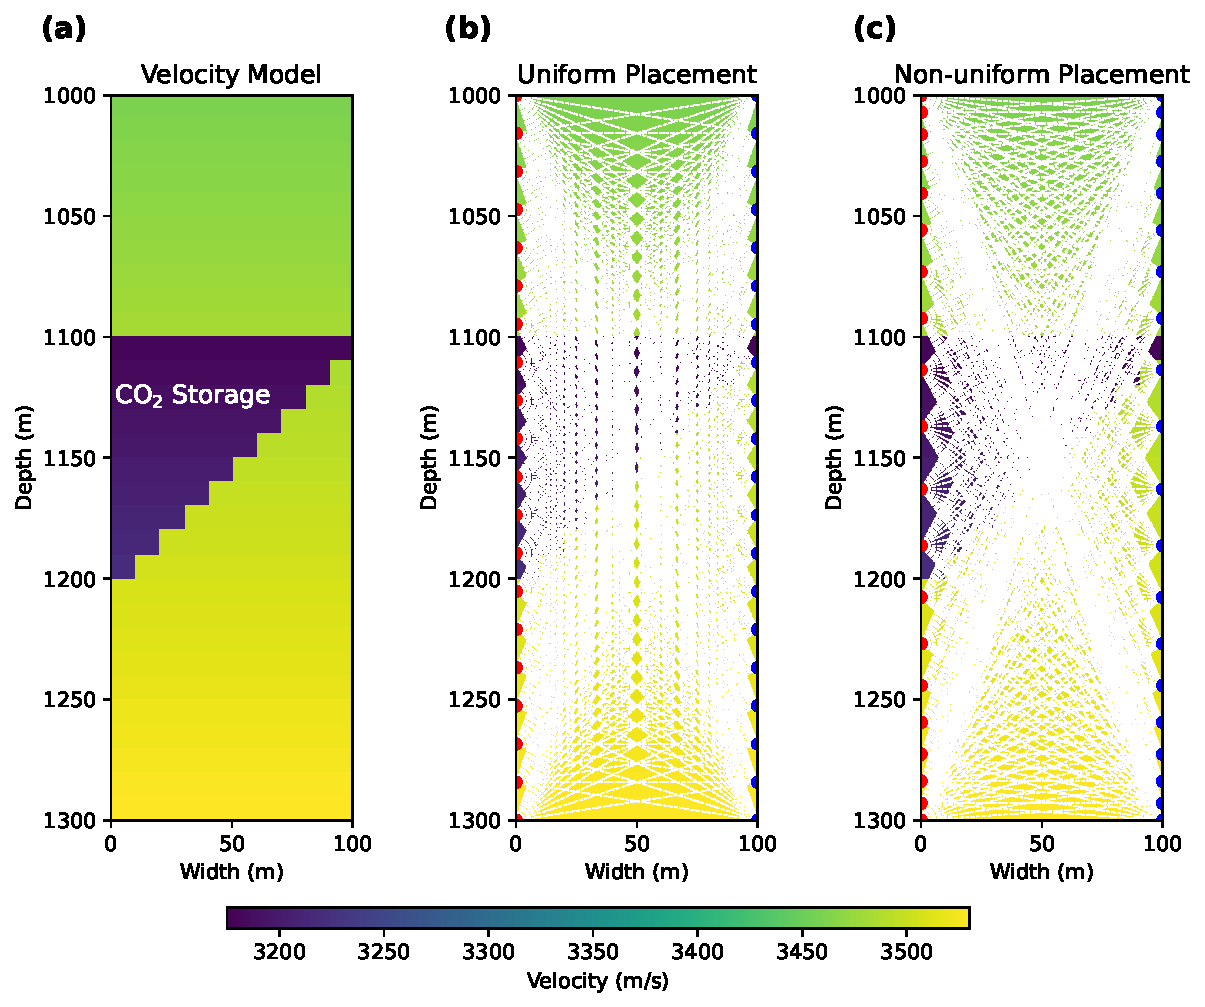
\includegraphics[width=0.8\linewidth]{chapter4/ray_coverage.pdf}
    \caption{The carbon storage velocity model and ray coverage patterns. Red dots are sources, blue dots are receivers, and white lines represent the ray paths. (a) The synthetic velocity model with a wedge-shaped low-velocity carbon storage formation. (b) Ray coverage from sources and receivers placed in a uniform grid within two boreholes. (c) Ray coverage from sources and receivers placed in a non-uniform pattern, enhancing coverage and constraints for the quantum annealing process.}
    \label{fig:ch3-ray-coverage}
\end{figure}

The uniform placement (\ref{fig:ch3-ray-coverage}b) is commonly used in seismic data acquisition for simplicity in boreholes. However, this approach results in significantly lower ray coverage in the shallow and deep sections compared to the middle section. To address these limitations, in our survey, 20 pairs of sources and receivers are non-uniformly deployed within two boreholes (\ref{fig:ch3-ray-coverage}c).
The non-uniform deployment is designed to introduce more constraints for the quantum annealing process, thereby improving the overall accuracy of the seismic inversion. The sources and receivers of non-uniform placement are distributed according to a quadratic polynomial distribution.

\subsubsection{Transforming Ray Equations to QUBO}

The set of ray equations can be represented as \cite{mcmechan83}:
\begin{equation}
\mathbf{D} \mathbf{s} = \mathbf{T},
\label{eq:ch3-ray-system}
\end{equation}
where $\mathbf{D}$ is the matrix of distance increments $d_j$, $\mathbf{s}$ is the slowness vector, and $\mathbf{T}$ is the travel time vector. The size of $\mathbf{D}$ can be very large, therefore solving for $\mathbf{s}$ through matrix operations on $\mathbf{D}$ is computationally intensive. This challenge is exacerbated by the relatively sparse and random distribution of elements within $\mathbf{D}$. Consequently, alternative methods are required to solve these problems efficiently while maintaining accuracy. Quantum annealers can provide quantum metaheuristic algorithms to address this issue. \Eqref{eq:ch3-ray-system} can be solved by minimizing the objective function:
\begin{equation}
f(\mathbf{s}) = \left\| \mathbf{D} \mathbf{s} - \mathbf{T} \right\|^2_2.
\label{eq:ch3-objective}
\end{equation}
The objective function \( f(\mathbf{s}) \) computes the difference between the observed travel times and those predicted by the model given a slowness vector $\mathbf{s}$. Minimizing this function ensures that the model's predictions align as closely as possible with the observed data, thus achieving an optimal fit.
Quantum annealers offer a direct approach to solving binary objective functions \cite{Omalley16}:
\begin{equation}
f(\mathbf{q}) = \left\| \mathbf{A}^d \mathbf{q} - \mathbf{b} \right\|^2_2.
\label{eq:ch3-binary-objective}
\end{equation}
In this formulation, $\mathbf{q}$ is a binary vector, $\mathbf{A}^d$ is a real-valued matrix, and $\mathbf{b}$ is a real-valued vector. Because quantum computers are designed to solve QUBO problems, transforming real-valued variables to binary values is essential. However, the number of binary variables $n_{\text{binary}}$ increases with the number of bits $R$ used for fixed-point approximation, and it is related to the number of real-valued variables $n_{\text{real}}$ as $n_{\text{binary}} = n_{\text{real}} \times R$.
Higher values of $R$ yield greater accuracy in representing the floating-point numbers, but the current limitations of quantum computer hardware restrict the number of qubits available. To address this issue without excessively increasing the number of binary variables, the initial velocity guess, variable boundaries \cite{Souza22} and recursive methods \cite{rogers20} are employed. The initial guess and the boundaries are used to rescale the range of the slowness vector $\mathbf{s}$ to a new vector $\mathbf{x}$ such that $x_i \in [0, 2)$, facilitating easier binary representation. Recursive methods are then applied to enhance the precision of floating-point divisions. These methods iteratively refine the estimate of $\mathbf{s}$, reducing the error at each step.
The initial objective function \Eqref{eq:ch3-objective} can be reformulated as:
\begin{equation}
f(\mathbf{x}) = \left\| \mathbf{D} \mathbf{x} - \mathbf{b} \right\|^2_2,
\end{equation}
where $\mathbf{b} = \left(\mathbf{T} + L \mathbf{I} - \mathbf{D} \mathbf{s}_0 \right) / L$, $L$ is the variable boundaries, $\mathbf{s}_0$ is the initial guess of the slowness vector, and $\mathbf{I}$ is the identity vector. The slowness vector $\mathbf{s}$ is then in the range of $[\mathbf{s}_0 - L \mathbf{I}; \mathbf{s}_0 + L \mathbf{I}]$. This range ensures that the solution space is adequately covered. To express this as a binary objective function, $x_i$ is represented in binary form using the $R$ bit fixed-point approximation:
\begin{equation}
x_i = \sum_{r=0}^{R-1} 2^{-r} q_r,
\label{eq:ch3-fixed-point}
\end{equation}
where $q_r \in \{0, 1\}$ is the value of the $r$-th bit. This transformation is essential for harnessing the computational power of quantum annealers, which are inherently designed to solve binary optimization problems. The new matrix $\mathbf{A}^d$ in \Eqref{eq:ch3-binary-objective} is derived from $\mathbf{D}$ and $R$ such that $\mathbf{D} \mathbf{x} = \mathbf{A}^d \mathbf{q}$. The QUBO matrix $Q_{ij}$ in \Eqref{eq:ch3-qubo} is then constructed from the given matrix $\mathbf{D}$ and the calculated vector $\mathbf{b}$ \cite{Omalley16,borle19}:
\begin{align}
Q_{jj} &= \sum_i A_{ij} (A_{ij} - 2b_j) , \\
Q_{jk} &= 2 \sum_i A_{ij} A_{ik} .
\end{align}
The QUBO matrix is directly input into the Quantum Processing Unit (QPU). The system utilizes \texttt{DWaveSampler()} to employ a D-Wave system as the sampler. Subsequently, \texttt{EmbeddingComposite()} manages the mapping between the problem and the D-Wave system's numerically indexed qubits, a process known as minor-embedding \cite{dwave23}.

In this study, we perform traveltime inversion using \(R=3\) for 10 iterations with quantum annealing. The total number of real-valued variables of the problem is 300. Due to quantum hardware limitations, we break down the model into 30 layers with 10 variables each. This division reduces the complexity of each sub-problem, making it manageable for the quantum processor and allowing for better control of the boundary \(L\). Since the problem from \Eqref{eq:ch3-ray-system} is depth-independent, we simplify the process by adjusting the system's coordinates at each iteration. The approach ensures that each layer is treated independently, reducing the overall complexity of the inversion. By implementing these techniques, we can efficiently solve large-scale traveltime inversion problems using quantum annealers.

\subsubsection{Tikhonov Regularization Linear Least Squares Inversion}

For ill-conditioned problems, small changes in \(\mathbf{D}\) or \(\mathbf{T}\) can lead to significant variations in the results \cite{Deif1986}. To mitigate the effects of noise in the data, we employ Tikhonov regularization methods. The new objective function (\Eqref{eq:ch3-objective}) can be expressed as a general regularized form \cite{fierro1997}:
\begin{equation}
f_\lambda(\mathbf{s}) = \| \mathbf{D} \mathbf{s} - \mathbf{T} \|_2^2 + \lambda g(\mathbf{s}),
\end{equation}
where \(\lambda\) is the regularization parameter controlling the trade-off between the data fidelity term \(\| \mathbf{D} \mathbf{s} - \mathbf{T} \|_2^2\) and the regularization term \(g(\mathbf{s})\). The Tikhonov regularization is flexible and allows different types of regularization functions. The standard Tikhonov regularization with \( L_2 \)-norm is in the form:
\begin{equation}
f_\lambda(\mathbf{s}) = \| \mathbf{D} \mathbf{s} - \mathbf{T} \|_2^2 + \lambda \|\mathbf{s}\|_2^2
\end{equation}
where \( \|\mathbf{s}\|_2^2 = \mathbf{s}^T \mathbf{s} \) penalizes large values in the solution. Another form is the first-order Tikhonov regularization with a smoothness regularization:
\begin{equation}
f_\lambda(\mathbf{s}) = \| \mathbf{D} \mathbf{s} - \mathbf{T} \|_2^2 + \lambda \| D_1 \mathbf{s} \|_2^2
\end{equation}
where \( D_1 \) is the first-order difference operator which enforces smooth variation in \( \mathbf{s} \) by penalizing large first derivatives. Similarly, second-order Tikhonov regularization penalizes the curvature of the solution:
\begin{equation}
f_\lambda(\mathbf{s}) = \| \mathbf{D} \mathbf{s} - \mathbf{T} \|_2^2 + \lambda \| D_2 \mathbf{s} \|_2^2
\end{equation}
where \( D_2 \) is the second-order difference operator which enforces smooth curvature by penalizing large second derivatives.
In general, \( g(\mathbf{s}) \) can be \( g(\mathbf{s}) = \|\mathbf{s}\|_2^2 \) for standard \( L_2 \)-norm regularization, \( g(\mathbf{s}) = \|D_1 \mathbf{s} \|_2^2 \) for first-order smoothness, or \( g(\mathbf{s}) = \|D_2 \mathbf{s} \|_2^2 \) for second-order smoothness. The choice of \( g(\mathbf{s}) \) depends on prior knowledge and the desired properties of the solution. Here, we use a custom Tikhonov regularization \(g(\mathbf{s}) = \| \mathbf{s} - \mathbf{s}_0 \|_2^2\), where \(\mathbf{s}_0\) is the initial guess for the slowness and is chosen as the input for the quantum annealing process. The objective function is now expressed as:
\begin{equation}
f_\lambda(\mathbf{s}) = \| \mathbf{D} \mathbf{s} - \mathbf{T} \|_2^2 + \lambda \| \mathbf{s} - \mathbf{s}_0 \|_2^2.
\end{equation}
The solution to this regularized problem is given by:
\begin{equation}
\mathbf{s} = \left( \mathbf{D}^T \mathbf{D} + \lambda \mathbf{I} \right)^{-1} \left( \mathbf{D}^T \mathbf{T} + \lambda \mathbf{s}_0 \right).
\label{eq:ch3-tikhonov-solution}
\end{equation}

\subsubsection{Cost Analysis}

Quantum annealing directly solves \(f(\mathbf{q}) = \left\| \mathbf{A}^d \mathbf{q} - \mathbf{b} \right\|^2_2\) (\Eqref{eq:ch3-binary-objective}) by providing the solution binary vector \(\mathbf{q}\). The quantum annealing process involves three sources of computational cost: preparing the binary problem, executing the annealing on the quantum hardware, and post-processing the results. The cost of preparing and post-processing is \(\mathcal{O}(mn^2 + mnc + n^2c^2)\). For a single iteration of the loop, the cost of executing the annealing process on the quantum hardware is \(\mathcal{O}(\mathcal{P}(cn))\). Here, \(m\) and \(n\) represent the rows and columns of the matrix \(\mathbf{D}\), respectively. \(\mathcal{P}(cn)\) is a polynomial term. The parameter \(c = |\Theta| + 1\), where \(\Theta\) used for representing the variables \(x_j\) as a fixed-point approximation in terms of power of 2 (\Eqref{eq:ch3-fixed-point}). The general form of the set \(\Theta\) is defined as \cite{borle19}:
\begin{equation}
    \Theta = \{ 2^l : l \in [o, p] \land l, o, p \in \mathbb{Z} \},
\end{equation}
where \(l\) is contiguous integer values within the interval \([o, p]\), and \(o\) and \(p\) are the lower and upper bounds of the interval. In our scheme, instead of using a large range for \(o\) and \(p\), we refine the precision of \(x_i\) iteratively over multiple loops to achieve higher accuracy. For a 3-bit fixed-point approximation with $x_i \in [0, 2)$, \(o = 0\) and \(p = -2\). For the \(K\) iterations, the total cost for  process is:
\begin{equation}
    \mathcal{O}(mn^2 + mnc + n^2c^2 + K\cdot\mathcal{P}(cn)),
    \label{eq:ch3-cost-annealing}
\end{equation}

For Tikhonov regularization methods with the direct solver (e.g., LU decomposition), the computational cost primarily depends on solving the modified linear system with the solution presented in \Eqref{eq:ch3-tikhonov-solution}. The cost for finding \(\mathbf{s}\) with a given \(\lambda\) is \(\mathcal{O}(mn^2 + n^3)\). Selecting the optimal \(\lambda\) is crucial for achieving a balance between data fidelity and regularization. One commonly used technique is the L-curve method, which plots the norm of the regularization term \(\|R(\mathbf{s})\|\) against the residual norm \(\|\mathbf{D} \mathbf{s} - \mathbf{T}\|\) on a log-log scale \cite{Hansen2000, CALVETTI2000423}. For \(N_\lambda\) values of \(\lambda\), the cost of solving the Tikhonov-regularized system for each \(\lambda\) is \( \mathcal{O}(N_\lambda \cdot (mn^2 + n^3))\). In addition, the computation of the residual norm \(\|\mathbf{D} \mathbf{s} - \mathbf{T}\|\) for each \(\lambda\) involves matrix-vector multiplications, contributing a cost of \(\mathcal{O}(N_\lambda \cdot mn)\). If we want to find the optimal \(\lambda\) automatically, the curvature of the L-curve must be computed. This requires additional operations such as numerical differentiation and curvature estimation, which are negligible compared to the cost of solving the regularized systems. Thus, the total cost for the L-curve method, including the automatic selection of \(\lambda\), is:
\begin{equation}
    \mathcal{O}(N_\lambda \cdot (mn^2 + n^3)).
    \label{eq:ch3-cost-tikhonov}
\end{equation}

From Equations \ref{eq:ch3-cost-annealing} and \ref{eq:ch3-cost-tikhonov}, achieving a computational cost of \(\mathcal{O}(\mathcal{P}(cn)) < \mathcal{O}(n^3)\) would enable quantum annealing to significantly accelerate problem-solving. Research efforts, such as those utilizing multi-qubit correction techniques \cite{dorband2018methodfindinglowerenergy}, aim to realize this improvement. These approaches can potentially achieve a substantial reduction in computational complexity. This advancement would facilitate rapid convergence to the global minimum and unlock considerable performance gains.

\subsection{Acknowledgments}

We would like to thank the Reservoir Characterization Project (RCP), Colorado School of Mines, for the financial support.

\subsection{Author Contributions}

H. A. Nguyen contributed to the methodology, formal analysis, writing of the manuscript, providing professional oversight and manuscript revision. A. Tura was responsible for conceptualization and manuscript revision.

\subsection{Competing Interests}

The authors declare no competing interests.

\subsection{Data Availability}

Access to the D-Wave System in this study is available at \href{https://cloud.dwavesys.com}{cloud.dwavesys.com}. The code related to this research be accessed at \href{https://github.com/x-repos/traveltime-inversion-annealing}{https://github.com/x-repos/traveltime-inversion-annealing}.

\chapter{Accelerating Physics-Informed Neural Networks for Full Waveform Inversion Using a Hybrid Quantum-Classical Finite-Basis Architecture}\label{chap:qufwi}

\begin{center}
    A paper submitted to \emph{IEEE Transactions on Geoscience and Remote Sensing}.

    Hoang Anh Nguyen\footnote{Department of Geophysics, Colorado School of Mines, Golden, Colorado 80401, USA\label{note:ch4-mines-geophysics}}$^,$\footnote{Primary researcher and author for correspondence},
    Divakar Vashisth\footnote{Department of Energy Science and Engineering, Stanford University, Stanford, California 94305, USA},
    and Ali Tura\footnote{Department of Petroleum Engineering, Colorado School of Mines, Golden, Colorado 80401, USA}
\end{center}

% Colors used by the TikZ schematic and the quantikz PQC diagram in this chapter.
\definecolor{classicalBlue}{RGB}{78,121,167}
\definecolor{quantumOrange}{RGB}{242,142,43}
\definecolor{outputGreen}{RGB}{89,161,79}
\definecolor{residualPurple}{RGB}{176,122,161}
\definecolor{neutralGray}{RGB}{120,120,120}

\subsection{Abstract}

Full waveform inversion (FWI) reconstructs heterogeneous material properties from receiver data but remains computationally demanding. Physics-informed neural networks (PINNs) and their domain-decomposed variants (FBPINNs) offer a mesh-free alternative but face convergence challenges when representing complex velocity fields. We present a hybrid quantum-classical FBPINN for acoustic FWI, bringing together quantum computing and classical machine learning, in which the decomposed wavefield network and the global velocity network are implemented as classical-to-quantum pipelines terminating in parameterized quantum circuits (PQCs). The PQCs are realized as differentiable JAX statevector simulators, enabling end-to-end automatic differentiation through the classical PINN, the quantum circuit, and the physics-informed loss. On a geophysical anomaly benchmark, the quantum hybrid reaches a lower L1 velocity error than the primary classical FBPINN baseline in approximately $8\times$ fewer training iterations, despite using approximately $33$\% fewer trainable parameters, and it outperforms all 15 classical hyperparameter variants tested. A second benchmark (checkerboard) demonstrates the generality of the inversion pipeline, confirming that the quantum hybrid architecture can recover structured spatial variations beyond the localized anomaly benchmark. Our framework is broadly applicable to wave-based inverse problems beyond geophysics, including medical ultrasound tomography and non-destructive evaluation.

\emph{Index Terms}: Quantum Computing, Full Waveform Inversion, Wave Propagation, Parameterized Quantum Circuit, PINNs.

\subsection{Introduction}

Full waveform inversion (FWI) is a powerful technique for reconstructing material properties from recorded waveform data by exploiting the full information content of wave signals, including amplitude, phase, and frequency. Originally developed in the context of exploration geophysics for subsurface velocity imaging~\cite{Tarantola1984}, FWI has since become central to a wide range of disciplines. In global seismology, it enables high-resolution imaging of crustal and mantle structures~\cite{Fichtner2009, Ebru2011}; in hydrocarbon exploration and CO$_2$ monitoring, it provides detailed velocity models for reservoir characterization~\cite{Virieux2009} and is increasingly applied to high-density datasets acquired via distributed acoustic sensing~\cite{Zhan2020}. Beyond geophysics, FWI principles have found growing applications in medical imaging, where ultrasound computed tomography employs waveform inversion to reconstruct tissue properties for breast cancer detection and characterization~\cite{10.1121/1.3699240, Sandhu_2015}, and in photoacoustic tomography, where wave-based inversion recovers optical absorption maps from acoustic measurements~\cite{Wang2016}. Non-destructive evaluation of engineering structures similarly leverages full waveform methods to detect defects and characterize material properties~\cite{7422116}. Despite its versatility across these domains, FWI remains computationally demanding, requiring iterative solutions of the forward wave equation and the computation of gradients through adjoint-state methods, often at substantial cost for large-scale and high-frequency problems. These computational demands have further motivated machine-learning surrogates for rapid waveform modeling and inversion~\cite{10091544}.

Physics-informed neural networks (PINNs) have emerged as a mesh-free alternative for solving partial differential equations (PDEs) by minimizing PDE residuals at collocation points~\cite{RAISSI2019686}, approximating solutions without traditional numerical discretization. This paradigm has been extended to inverse problems, where unknown model parameters are optimized alongside the solution. Recent works have applied PINNs to wave-related problems~\cite{10.1093/gji/ggab010, waheed2021pinntomoseismictomographyusing, 10230537}, offering a fundamentally different approach to the classical adjoint-state framework. In particular, Rasht-Behesht \emph{et al.}~\cite{rahst} demonstrated the application of PINNs to FWI, achieving accurate velocity reconstruction from receiver data by jointly optimizing the wavefield and velocity networks. Physics-informed formulations have since been applied to seismic inversion through the acoustic wave equation~\cite{10017252}, while purely data-driven networks instead learn a direct mapping from seismic data to subsurface velocity models~\cite{8931232, 9044635}. However, standard PINNs face well-documented challenges when applied to problems involving high-frequency wave propagation, multi-scale physics, and large computational domains. The spectral bias of neural networks, their tendency to learn low-frequency features before high-frequency ones, can severely limit convergence in wave propagation problems. To address these limitations, finite-basis physics-informed neural networks (FBPINNs) were introduced by Moseley \emph{et al.}~\cite{Moseley2023}, employing a domain decomposition strategy in which the global solution is represented as a sum of locally supported basis functions, each parameterized by an independent neural network. This approach effectively mitigates spectral bias, improves parallel scalability, and enables the solution of problems that are intractable for standard PINNs. To date, however, no work has applied the domain decomposition advantages of FBPINNs to waveform inversion.

In parallel with advances in classical scientific machine learning, quantum computing has attracted growing interest for its potential to accelerate computational tasks across diverse domains. Parameterized quantum circuits (PQCs), also known as variational quantum circuits (VQCs), have emerged as a near-term approach to quantum machine learning, operating within the constraints of current noisy intermediate-scale quantum (NISQ) devices~\cite{Preskill2018quantumcomputingin}. PQCs encode classical data into quantum states through feature maps, process the information through parameterized unitary operations, and extract classical outputs via measurement. Several studies have explored the integration of quantum circuits with neural networks, forming hybrid quantum-classical architectures that leverage the expressive power of quantum Hilbert spaces while maintaining the trainability and flexibility of classical networks~\cite{PhysRevA.101.032308, Benedetti_2019, Ostaszewski2021structure}.

The intersection of quantum computing and PINNs has begun to receive attention, with recent works investigating quantum physics-informed neural networks (QPINNs) for solving differential equations~\cite{https://doi.org/10.1002/qute.202300065}. Leong \emph{et al.}~\cite{LEONG2025106782} benchmarked hybrid quantum physics-informed neural networks (HQPINNs) for high-speed flow problems, demonstrating that these architectures offer competitive accuracy and stability with a reduced parameter cost compared to classical PINNs. While they found that pure quantum models struggle with non-harmonic features like shocks, the hybrid approach successfully mitigates these artifacts by leveraging classical sub-networks. Similarly, Berger \emph{et al.}~\cite{Berger2025} proposed trainable embedding quantum physics-informed neural networks (TE-QPINNs) for solving nonlinear PDEs, including the Navier-Stokes equations. Their approach achieved superior results compared to classical PINNs while maintaining the same number of parameters, highlighting the potential for more efficient optimization in high-dimensional parameter spaces. These studies suggest that quantum circuits can serve as powerful function approximators within the PINN framework, potentially offering advantages in expressivity and parameter efficiency for forward PDE problems. Complementing these variational formulations, direct gate-based quantum algorithms have also been developed to solve PDEs without a learned model, with explicit circuit constructions for the acoustic wave equation and related operators~\cite{tbzc-w9x8} and a demonstration of one-dimensional wave-equation simulation on near-term quantum hardware~\cite{PhysRevResearch.6.043169}. When extending quantum methods to geophysical inverse problems, research has thus far primarily relied on alternative computing paradigms. For instance, quantum annealing has recently been applied to seismic traveltime tomography~\cite{Nguyen2025} and to pre-stack and post-stack seismic inversion~\cite{Vashisth2025GEO}, with the inverse problem cast as a least-squares objective, mapped to a quadratic unconstrained binary optimization (QUBO) or Ising Hamiltonian formulation, and solved using a quantum annealer. More recently, hybrid quantum neural networks have also been explored for pre-stack and post-stack seismic inversion within physics-informed encoder-decoder architectures~\cite{Vashisth2025HQNN}. However, the application of gate-based hybrid quantum-classical neural architectures to highly nonlinear inverse problems like FWI, where both the wavefield and the velocity model are represented by learned networks and coupled through the acoustic wave equation, remains largely unexplored.

In this work, we present, to the best of our knowledge, the first application of gate-based quantum computing to full waveform inversion: a hybrid quantum-classical FBPINN for acoustic FWI. The framework represents both the decomposed wavefield network and the global velocity network by classical-to-quantum pipelines: classical pre-networks map the input coordinates into low-dimensional latent spaces matched to the number of qubits, the PQCs process the encoded features through parameterized rotations and entangling gates, and classical output layers rescale the bounded circuit outputs into physical units. To isolate the architectural benefits of the quantum integration from the hardware noise of current near-term devices, the PQCs are implemented as JAX-native statevector simulators. This approach enables exact, end-to-end automatic differentiation through the classical PINN, the quantum circuit, and the physics-informed loss, avoiding the prohibitive computational overhead of parameter-shift rules required on physical hardware. This design combines the scalability advantages of FBPINN domain decomposition with the structured, bounded expressivity of PQC-based parameterizations. We evaluate the architecture on two geophysical benchmarks and compare it against a purely classical FBPINN baseline as well as 15 classical hyperparameter variants. In the following sections, we present the comparative performance of our hybrid architecture, discuss its broader implications for scientific machine learning, and detail the underlying mathematical and algorithmic methodology.

\subsection{Methodology}\label{sec:ch4-method}

\subsubsection{Acoustic wave equation}
\label{sec:ch4-methods-wave}

Two-dimensional acoustic wave propagation in a heterogeneous medium with spatially varying wave speed $\alpha(\mathbf{x})$ and constant density is governed by the acoustic wave equation
\begin{equation}
\frac{\partial^{2} \phi(\mathbf{x},t)}{\partial t^{2}}
= \alpha^{2}(\mathbf{x})\,\nabla^{2} \phi(\mathbf{x},t) + s(\mathbf{x},t),
\label{eq:ch4-acoustic-wave}
\end{equation}
where $\phi(\mathbf{x},t)$ is the scalar displacement potential, $\nabla^2$ is the spatial Laplacian, and $s(\mathbf{x},t)$ is the seismic source. The spatial gradient of $\phi$ yields the physical displacement field.

In the context of FWI, the objective is to reconstruct the unknown wave speed $\alpha(\mathbf{x})$ from surface observations. Within our PINN architecture, to avoid the numerical challenges of explicitly modeling the source singularity $s(\mathbf{x},t)$, the source is instead encoded through the initial conditions. This is achieved by specifying the wavefield at two closely spaced early times, derived from a spectral-element forward simulation~\cite{11367068}. The top boundary of the domain acts as a free surface where the acoustic pressure vanishes, which is mathematically equivalent to $\nabla^2 \phi = 0$ in this displacement-potential formulation.

Accordingly, the source-free form of \Eqref{eq:ch4-acoustic-wave} is enforced as a PDE residual at interior collocation points, while the initial states and free-surface boundary conditions are imposed as soft constraints within the training loss. The measured receiver data are incorporated as an additional data-misfit term, penalizing the discrepancy between the predicted wavefield at receiver locations and the observed seismograms. The complete composite loss function used to train the FBPINN is detailed in the Hybrid architecture section.

\subsubsection{Finite-basis physics-informed neural network}
\label{sec:ch4-methods-fbpinn}

PINNs~\cite{RAISSI2019686} approximate solutions of PDEs by a neural network $u_\theta(\mathbf{x})$ and train $\theta$ to minimize the PDE residual at a set of collocation points $\{\mathbf{x}_i\}_{i=1}^{N}$ drawn from the domain. Writing the governing PDE in residual form $\mathcal{N}[u](\mathbf{x}) = 0$, the PDE loss is
\begin{equation}
    \mathcal{L}_\text{PDE}
    = \frac{1}{N} \sum_{i=1}^{N}
    \left| \mathcal{N}[u_\theta(\mathbf{x}_i)] \right|^{2},
\end{equation}
with spatial and temporal derivatives computed by automatic differentiation of the network with respect to its inputs. Boundary conditions, initial conditions, and observational data are added as additional weighted loss terms (the full composite loss used for FWI is given in the Hybrid architecture subsection below). Standard PINNs, however, are known to suffer from spectral bias, a tendency to learn low-frequency features before high-frequency ones, which severely limits their effectiveness in multi-scale wave problems such as FWI, where both the velocity field and the wavefield exhibit sharp transitions and oscillatory structure.

To overcome this limitation, we adopt the FBPINN framework of Moseley \emph{et al.}~\cite{Moseley2023}. The global domain $\Omega$ is partitioned into $K$ overlapping rectangular subdomains $\{\Omega_k\}$, each equipped with an independent neural network $u_{\theta_k}(\mathbf{x})$. The global solution is reconstructed as a partition-of-unity sum,
\begin{equation}
    u(\mathbf{x}) = \sum_{k=1}^{K} w_k(\mathbf{x})\, u_{\theta_k}(\mathbf{x}),
\end{equation}
where the window functions $w_k$ are smooth cosine bumps supported on $\Omega_k$ with $\sum_k w_k(\mathbf{x}) = 1$ for all $\mathbf{x} \in \Omega$. Each local network only needs to represent the solution's behavior on its own subdomain, with two consequences: (i) the local frequency content each network must learn is bounded by the subdomain size, alleviating spectral bias; and (ii) training is embarrassingly parallel across subdomains. The physics-informed loss is evaluated on the reconstructed global solution, so gradients flow through the window-weighted sum back to the individual subdomain networks.

For the wavefield $\phi(x,z,t)$ we use a three-dimensional subdomain decomposition $(n_x, n_z, n_t)$, $5\!\times\!3\!\times\!5$ in the anomaly baseline with subdomain overlap $0.35$. The velocity network $\alpha(x,z)$ is not decomposed; it is a single global network, since the velocity field typically varies more smoothly than the wavefield and does not require local representation.

\subsubsection{Parameterized quantum circuits}
\label{sec:ch4-methods-pqc}

We first summarize the quantum-computing concepts used by the hybrid architecture. A single qubit is a two-level quantum system with state
\begin{equation}
  |\psi\rangle = c_0\,|0\rangle + c_1\,|1\rangle, \qquad
  |c_0|^2 + |c_1|^2 = 1,
\end{equation}
where $c_0,c_1 \in \mathbb{C}$ are probability amplitudes. An $n$-qubit register is represented by a normalized statevector in $\mathbb{C}^{2^n}$,
\begin{equation}
  |\psi\rangle = \sum_{k=0}^{2^n-1} c_k\,|k\rangle, \qquad
  \sum_{k=0}^{2^n-1} |c_k|^2 = 1.
\end{equation}
The parameterized single-qubit rotations used in this work are
\begin{equation}
  R_k(\theta)=e^{-i\theta\,\sigma_k/2}, \qquad k\in\{x,y,z\},
\end{equation}
with explicit matrices
\begin{equation}
\begin{aligned}
  R_x(\theta) &=
  \begin{pmatrix} \cos\tfrac{\theta}{2} & -i\sin\tfrac{\theta}{2} \\
  -i\sin\tfrac{\theta}{2} & \cos\tfrac{\theta}{2} \end{pmatrix},
  \\
  R_y(\theta) &=
  \begin{pmatrix} \cos\tfrac{\theta}{2} & -\sin\tfrac{\theta}{2} \\
  \sin\tfrac{\theta}{2} & \cos\tfrac{\theta}{2} \end{pmatrix},
  \\
  R_z(\theta) &=
  \begin{pmatrix} e^{-i\theta/2} & 0 \\
  0 & e^{i\theta/2} \end{pmatrix}.
\end{aligned}
\end{equation}
The composition $R_z(\theta_3)R_y(\theta_2)R_x(\theta_1)$ spans $\mathrm{SU}(2)$ and can prepare any single-qubit pure state up to a physically irrelevant global phase. Entanglement between neighbouring qubits is introduced by the controlled-NOT (CNOT) gate,
\begin{equation}
  \mathrm{CNOT} =
  \begin{pmatrix} 1 & 0 & 0 & 0 \\
                  0 & 1 & 0 & 0 \\
                  0 & 0 & 0 & 1 \\
                  0 & 0 & 1 & 0 \end{pmatrix},
\end{equation}
which flips the target qubit if and only if the control qubit is in state $|1\rangle$.

A PQC~\cite{Benedetti_2019} applies a trainable unitary $U(\boldsymbol{\theta}_q)$ to the initial state $|0\rangle^{\otimes n}$ and returns a scalar expectation value of a Hermitian observable, yielding a smooth, differentiable function of the circuit parameters $\boldsymbol{\theta}_q$. Its expressibility depends on the circuit depth, qubit connectivity, and gate set~\cite{sim2019expressibility}.

The PQC employed in this work (\ref{fig:ch4-pqc-architecture}) operates on $n$ qubits with $L$ variational layers. In the data-embedding layer, starting from $|0\rangle^{\otimes n}$, each qubit $i$ receives an $R_y(\beta_i\, z_i)$ rotation that encodes the $i$-th component of the input vector $\mathbf{z} \in \mathbb{R}^n$ as a rotation angle (angle encoding~\cite{schuld2021machine}), scaled by a trainable basis parameter $\beta_i$:
\begin{equation}
  |\psi_\mathrm{enc}(\mathbf{z};\boldsymbol{\beta})\rangle = \bigotimes_{i=0}^{n-1} R_y(\beta_i\, z_i)\,|0\rangle.
\end{equation}
This is followed by $L$ variational layers. Each layer $l = 1, \ldots, L$ applies a general single-qubit rotation $R_z(\theta^{(3)}_{l,i})\, R_y(\theta^{(2)}_{l,i})\, R_x(\theta^{(1)}_{l,i})$ to every qubit $i$, introducing $3n$ trainable parameters per layer, and then applies a linear CNOT ladder $\text{CNOT}(i, i{+}1)$ for $i = 0, \ldots, n{-}2$ to entangle neighboring qubits. The total number of trainable gate parameters is $3nL$, plus $n$ basis parameters from the embedding layer. In the measurement layer, the Pauli-$Z$ expectation values $\langle Z_i \rangle$ on each qubit are averaged to produce a single scalar output
\begin{equation}
  f(\mathbf{z}; \boldsymbol{\beta}, \boldsymbol{\theta}_q)
  = \frac{1}{n} \sum_{i=0}^{n-1} \langle\psi(\mathbf{z}; \boldsymbol{\beta}, \boldsymbol{\theta}_q)|\, Z_i \,|\psi(\mathbf{z}; \boldsymbol{\beta}, \boldsymbol{\theta}_q)\rangle
  \;\in [-1,\, 1].
  \label{eq:ch4-pqc-output}
\end{equation}

The three design choices of this output head, angle encoding with trainable scales, a hardware-efficient variational block, and a local averaged read-out, are each motivated below; their representational consequences are taken up quantitatively in the Discussion and Section~\ref{app:ch4-fourier}. The encoding rotation $R_y(\beta_i z_i)$ rotates qubit $i$ by an angle linear in the latent component $z_i$, so each coordinate enters the state through a bounded, smooth map whose dependence on $z_i$ is periodic in the encoded angle. Making the per-qubit scale $\beta_i$ a trainable parameter lets the circuit adapt the frequencies through which the latent variables are read out, a role analogous to learned input scalings in classical coordinate networks~\cite{schuld2021machine}; for angle-encoded circuits this produces a finite-frequency (Fourier) structure in $\mathbf{z}$ whose accessible frequencies are set by $\boldsymbol{\beta}$~\cite{schuld2021effect}.

Each variational layer is a hardware-efficient ansatz~\cite{cerezo2021variational,kandala2017hardware}: a universal single-qubit rotation $R_z\,R_y\,R_x$ on every qubit, which spans $\mathrm{SU}(2)$ and so imposes no a~priori restriction on the local state ($3n$ angles per layer), interleaved with a linear nearest-neighbour CNOT ladder. We adopt this structure because it is built only from one- and two-qubit gates on adjacent wires, the native low-overhead operations on most physical architectures~\cite{Preskill2018quantumcomputingin,kandala2017hardware}, and because the expressibility and entangling capacity of this gate family have been characterised at modest depth~\cite{sim2019expressibility,Benedetti_2019}. The averaged observable $f=\tfrac{1}{n}\sum_i\langle Z_i\rangle$ is correspondingly a sum of single-qubit (weight-one) Pauli terms rather than a global, high-weight observable; as a network head each $\langle Z_i\rangle\in[-1,1]$ yields a single scalar bounded in $[-1,1]$ that the subsequent affine layer rescales to physical units. The compactness of this $3nL+n$-angle parameterization comes with a known trainability caveat: deep or globally measured hardware-efficient circuits can exhibit barren plateaus (vanishingly small gradients)~\cite{mcclean2018barren}, and the severity of this effect depends on the locality of the cost~\cite{cerezo2021costfunction}. The small width ($n=4$), shallow depth ($L=2$), and local read-out used here are the regime in which such gradients are least suppressed, and the differentiable statevector simulation of backpropagates through the circuit directly, without parameter-shift estimators.

These arguments concern inductive bias, parameter efficiency, and trainability, not any computational speedup. The circuit is evaluated by exact JAX statevector simulation and, because its output is a finite-frequency function of $\mathbf{z}$, the realized function class is in principle classically representable; we make no claim of quantum advantage. We further note that capacity is not concentrated in one wide entangled register: the architecture instantiates $76$ independent four-qubit PQCs, one per wavefield subdomain ($5\!\times\!3\!\times\!5$) plus one for the global velocity network, each carrying its own angles $(\boldsymbol{\beta},\boldsymbol{\theta}_q)$, so the per-circuit width stays fixed at four qubits as the subdomain decomposition is refined.

\def\myvdots{\ \vdots\ }
\def\myddots{\ \ddots\ }
\begin{figure}[!t]
\centering
\resizebox{\linewidth}{!}{
    \begin{quantikz}
    \lstick{$\ket{q_1}$}
        & \gate[style={draw=classicalBlue!75!black, fill=classicalBlue!12}]{R_y(\beta_1 z_1)}
            \gategroup[5,steps=1,style={dashed, draw=classicalBlue!70!black, fill=classicalBlue!8, rounded corners, inner xsep=2pt},background,
            label style={label position=below,anchor=north,yshift=-0.2cm}]
            {{\textbf{Encoding}}}
        & \gate[style={draw=quantumOrange!80!black, fill=quantumOrange!14}]{R_x(\theta^{(1)}_{l,1})}
            \gategroup[5,steps=7,style={dashed, draw=quantumOrange!75!black, fill=quantumOrange!9, rounded corners, inner xsep=2pt},background,
            label style={label position=below,anchor=north,yshift=-0.2cm}]
            {{\textbf{Repeat $L$ times}}}
        & \gate[style={draw=quantumOrange!80!black, fill=quantumOrange!14}]{R_y(\theta^{(2)}_{l,1})}
        & \gate[style={draw=quantumOrange!80!black, fill=quantumOrange!14}]{R_z(\theta^{(3)}_{l,1})}
        & \ctrl{1} & & & & \meter[style={draw=outputGreen!70!black, fill=outputGreen!12}]{} \\
    \lstick{$\ket{q_2}$}
        & \gate[style={draw=classicalBlue!75!black, fill=classicalBlue!12}]{R_y(\beta_2 z_2)}
        & \gate[style={draw=quantumOrange!80!black, fill=quantumOrange!14}]{R_x(\theta^{(1)}_{l,2})}
        & \gate[style={draw=quantumOrange!80!black, fill=quantumOrange!14}]{R_y(\theta^{(2)}_{l,2})}
        & \gate[style={draw=quantumOrange!80!black, fill=quantumOrange!14}]{R_z(\theta^{(3)}_{l,2})}
        & \targ{}
        & \ctrl{1} & & & \meter[style={draw=outputGreen!70!black, fill=outputGreen!12}]{}\\
    \lstick{$\ket{q_3}$}
        & \gate[style={draw=classicalBlue!75!black, fill=classicalBlue!12}]{R_y(\beta_3 z_3)}
        & \gate[style={draw=quantumOrange!80!black, fill=quantumOrange!14}]{R_x(\theta^{(1)}_{l,3})}
        & \gate[style={draw=quantumOrange!80!black, fill=quantumOrange!14}]{R_y(\theta^{(2)}_{l,3})}
        & \gate[style={draw=quantumOrange!80!black, fill=quantumOrange!14}]{R_z(\theta^{(3)}_{l,3})}
        & & \targ{}
        & \ctrl{1}
        & & \meter[style={draw=outputGreen!70!black, fill=outputGreen!12}]{} \\
    \setwiretype{n} \myvdots
        & \myvdots & \myvdots & \myvdots & \myvdots
        & \myvdots & \myvdots & \myddots & \myddots & \myvdots \\
    \lstick{$\ket{q_n}$}
        & \gate[style={draw=classicalBlue!75!black, fill=classicalBlue!12}]{R_y(\beta_n z_n)}
        & \gate[style={draw=quantumOrange!80!black, fill=quantumOrange!14}]{R_x(\theta^{(1)}_{l,n})}
        & \gate[style={draw=quantumOrange!80!black, fill=quantumOrange!14}]{R_y(\theta^{(2)}_{l,n})}
        & \gate[style={draw=quantumOrange!80!black, fill=quantumOrange!14}]{R_z(\theta^{(3)}_{l,n})}
        & & & & \targ{} & \meter[style={draw=outputGreen!70!black, fill=outputGreen!12}]{}
    \end{quantikz}
}
\caption{Multilayer PQC $\mathcal{Q}$. Each input feature $z_i$ is angle-encoded via an $R_y(\beta_i\, z_i)$ rotation (blue encoding layer), where $\beta_i$ is a trainable scaling parameter. Variational layers of single-qubit rotations $R_x$, $R_y$, $R_z$ followed by a linear CNOT ladder are repeated $L$ times (orange block). Each qubit is measured in the Pauli-$Z$ basis (green meters), and the outputs are averaged to yield a scalar in $[-1, 1]$.}
\label{fig:ch4-pqc-architecture}
\end{figure}

\subsubsection{JAX-based statevector simulator}
\label{sec:ch4-methods-statevector}

We implement the PQC as a lightweight statevector simulator in JAX~\cite{jax2018github} rather than relying on an external framework such as PennyLane~\cite{bergholm2022pennylaneautomaticdifferentiationhybrid} or Qiskit~\cite{javadiabhari2024quantumcomputingqiskit}. The simulator represents the quantum state as a $2^n$-dimensional complex vector and applies gate operations via tensor contractions: single-qubit rotation gates ($R_x$, $R_y$, $R_z$) are constructed as $2\!\times\!2$ unitary matrices and applied with \texttt{jnp.tensordot} on the reshaped state tensor, and CNOT gates are realized through index permutation and conditional flipping on the control-target subspace. Expectation values are computed analytically from the statevector amplitudes, without stochastic sampling, as in PennyLane's \texttt{default.qubit} backend.

On near-term quantum hardware, gradients of PQC outputs with respect to gate parameters are typically computed via the parameter-shift rule~\cite{mitarai2018quantum,schuld2019evaluating}, which evaluates the circuit at two shifted parameter values per gate and therefore requires $2p$ circuit evaluations per gradient for a circuit with $p$ parameters. In classical statevector simulation, each gate application is already a standard differentiable operation, so embedding the circuit in JAX offers two concrete advantages. First, \texttt{jax.grad} and \texttt{jax.jvp} backpropagate through the full hybrid pipeline (classical PINN layers, quantum circuit, and loss function) without parameter-shift rules or cross-framework bridging. Second, the entire training loop can be compiled into a single optimized XLA program via \texttt{jax.jit}, eliminating Python-level dispatch and framework-bridging overhead. The trade-off is the exponential cost of representing the quantum state explicitly: the simulator holds all $2^n$ complex amplitudes, giving $\mathcal{O}(2^n)$ memory, and applies $\mathcal{O}(Ln)$ gates that each sweep the full state, giving $\mathcal{O}(L\,n\,2^n)$ computation. This limits the approach to moderate qubit counts; for the circuit sizes used here ($n \leq 8$, $L \leq 6$), this cost is negligible compared with the classical network and loss evaluation. We verify numerical correctness by comparing parameter gradients $\partial f/\partial\boldsymbol{\theta}_q$ against PennyLane's \texttt{default.qubit} backend~\cite{bergholm2022pennylaneautomaticdifferentiationhybrid} across eight circuit configurations (2--8 qubits, 1--6 layers); the maximum absolute deviation is below $2\times 10^{-7}$, consistent with \texttt{float32} machine precision (\ref{fig:ch4-pqc-gradient}).

\begin{figure}[!t]
\centering
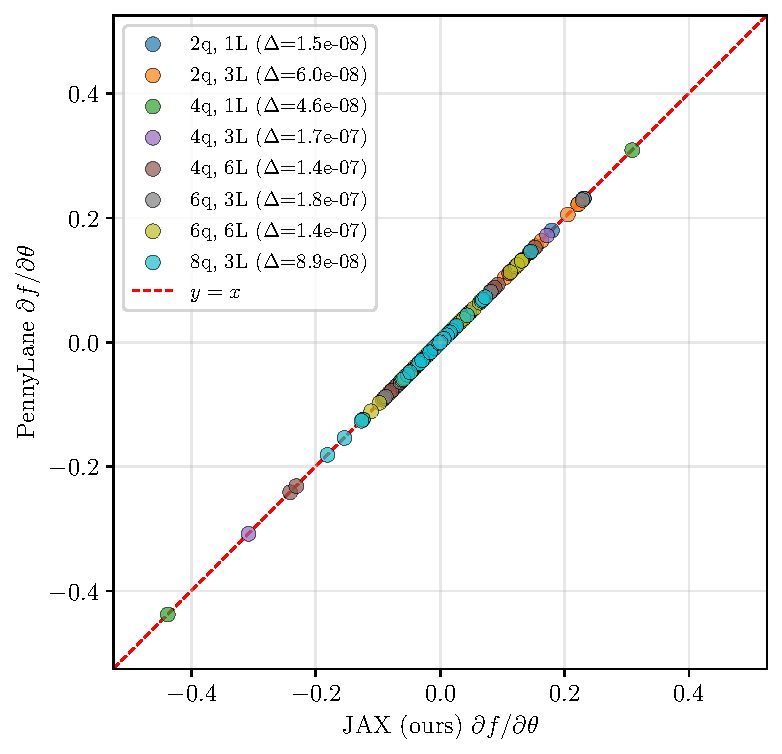
\includegraphics[width=\linewidth]{chapter5/pqc_gradient_agreement.pdf}
\caption{Comparison of parameter gradients $\partial f / \partial \boldsymbol{\theta}_q$ computed by our JAX statevector implementation and PennyLane's \texttt{default.qubit} backend across eight circuit configurations (2--8 qubits, 1--6 layers). All values fall on the identity line $y = x$ with maximum absolute deviation $\Delta < 2\times 10^{-7}$, confirming numerical equivalence of the two implementations.}
\label{fig:ch4-pqc-gradient}
\end{figure}

\subsubsection{Hybrid quantum-classical architecture}\label{sec:ch4-hybrid-network}

\begin{figure}[!t]
\centering
\resizebox{\linewidth}{!}{%
\begin{tikzpicture}[
  >=Stealth,
  font=\Large,
  node distance=2.2cm and 2.4cm,
  box/.style={draw=classicalBlue!70!black, rounded corners, line width=0.9pt, minimum width=3.0cm, minimum height=1.0cm, align=center, fill=classicalBlue!10},
  qbox/.style={draw=quantumOrange!80!black, rounded corners, line width=0.9pt, minimum width=3.0cm, minimum height=1.0cm, align=center, fill=quantumOrange!14},
  circ/.style={circle, draw=outputGreen!70!black, line width=0.9pt, minimum size=30, fill=outputGreen!14},
  loss/.style={ellipse, draw=residualPurple!80!black, line width=0.9pt, minimum width=1.8cm, minimum height=1.0cm, align=center, fill=residualPurple!14},
  data/.style={draw=residualPurple!80!black, rounded corners, line width=0.9pt, minimum width=3.0cm, minimum height=1.0cm, align=center, fill=residualPurple!10},
  physmain/.style={draw=residualPurple!80!black, rounded corners, line width=0.9pt, minimum width=4.0cm, minimum height=2.0cm, align=left, fill=residualPurple!8},
  decision/.style={diamond, draw=neutralGray!85!black, aspect=2, minimum width=1.6cm, inner sep=1pt, align=center, fill=neutralGray!10},
  neuron/.style={circle, draw=classicalBlue!70!black, fill=classicalBlue!12, minimum size=5mm, inner sep=0pt},
  inlabel/.style={circle, draw=classicalBlue!75!black, fill=classicalBlue!22, minimum size=7mm, inner sep=0pt, font=\small},
  nconn/.style={draw=classicalBlue!35, line width=0.3pt}
]

% --- NODES ---
% ===== Wavefield classical pre-network (MLP), inputs (x,z,t) =====
\node[inlabel] (wi1) at (0,0.7) {$x$};
\node[inlabel] (wi2) at (0,0.0) {$z$};
\node[inlabel] (wi3) at (0,-0.7) {$t$};
\foreach \i/\y in {1/1.05,2/0.35,3/-0.35,4/-1.05}{ \node[neuron] (wha\i) at (1.15,\y) {}; }
\foreach \i/\y in {1/1.05,2/0.35,3/-0.35,4/-1.05}{ \node[neuron] (whb\i) at (2.3,\y) {}; }
\foreach \a in {1,2,3}{\foreach \b in {1,2,3,4}{\draw[nconn] (wi\a)--(wha\b);}}
\foreach \a in {1,2,3,4}{\foreach \b in {1,2,3,4}{\draw[nconn] (wha\a)--(whb\b);}}
\node[draw=none, inner sep=2pt, fit=(wi1)(wi3)(whb1)(whb4)] (net1) {};
\node[anchor=north] (net1lab) at (1.15,-1.45) {$\mathcal{N}_\phi(x,z,t)$};
\node[qbox, right=1.cm of net1] (qc1) {$\mathcal{Q}_\phi(\mathcal{N}_\phi)$};
\node[circ, right=1.5cm of qc1] (phi) {$\phi$};

% --- DATA RESIDUAL BOX: label on top, observed (solid) vs predicted (dashed) seismograms below ---
\node[draw=residualPurple!80!black, rounded corners, line width=0.9pt, fill=residualPurple!10,
      minimum width=5.0cm, minimum height=2.8cm, right=3.0cm of phi] (data) {};
\node[anchor=north, font=\Large] at ([yshift=-0.16cm]data.north) {Data residual: $\mathcal{R}_{\mathrm{data}}$};
\begin{scope}[shift={(data.south west)}]
  \foreach \y in {0.45, 1.0, 1.55}{
    \draw[neutralGray!40, line width=0.4pt] (0.45,\y) -- (4.55,\y);
    \draw[residualPurple!75!black, line width=0.9pt, smooth, samples=120, domain=0.45:4.55]
      plot (\x, {\y + 0.22*sin(360*1.15*\x)*exp(-((\x-2.5)^2)/0.9)});
    \draw[quantumOrange!85!black, line width=0.9pt, dashed, smooth, samples=120, domain=0.45:4.55]
      plot (\x, {\y + 0.19*sin(360*1.15*\x + 30)*exp(-((\x-2.58)^2)/1.0)});
  }
\end{scope}
\node[physmain, below=1.5cm of data] (phys)
{PDE residual: $\mathcal{R}_{\mathrm{PDE}}(\phi,\alpha)=\partial_{tt}\phi-\alpha^2\nabla^2\phi$\\
BC residual: $\mathcal{R}_{\mathrm{BC}}(\phi,\alpha)$\\
IC residual: $\mathcal{R}_{\mathrm{IC}}(\phi,\alpha)$\\
Parameter constraints / bounds on $\alpha$};
\node[loss, right=1.5cm of phys] (loss) {$\mathcal{L}_{\mathrm{total}}$};

\coordinate (phys_lower) at ([yshift=-0.85cm]phys.center);
% ===== Velocity classical pre-network (MLP), inputs (x,z) =====
\coordinate (vbase) at (wi2 |- phys_lower);
\node[inlabel] (vi1) at ([yshift=0.35cm]vbase) {$x$};
\node[inlabel] (vi2) at ([yshift=-0.35cm]vbase) {$z$};
\foreach \i/\y in {1/1.05,2/0.35,3/-0.35,4/-1.05}{ \node[neuron] (vha\i) at ([xshift=1.15cm,yshift=\y cm]vbase) {}; }
\foreach \i/\y in {1/1.05,2/0.35,3/-0.35,4/-1.05}{ \node[neuron] (vhb\i) at ([xshift=2.3cm,yshift=\y cm]vbase) {}; }
\foreach \a in {1,2}{\foreach \b in {1,2,3,4}{\draw[nconn] (vi\a)--(vha\b);}}
\foreach \a in {1,2,3,4}{\foreach \b in {1,2,3,4}{\draw[nconn] (vha\a)--(vhb\b);}}
\node[draw=none, inner sep=2pt, fit=(vi1)(vi2)(vhb1)(vhb4)] (net2) {};
\node[anchor=north] (net2lab) at ([xshift=1.15cm,yshift=-1.45cm]vbase) {$\mathcal{N}_\alpha(x,z)$};
\node[qbox, right=1.cm of net2] (qc2) {$\mathcal{Q}_\alpha(\mathcal{N}_\alpha)$};
\node[circ, right=1.5cm of qc2] (cvar) {$\alpha$};

% --- BACKGROUND BOX ---
\begin{scope}[on background layer]
    % Invisible bounding box to maintain layout alignment for later nodes
    \node[inner sep=15pt, fit=(net1) (net2) (qc1) (qc2)] (hybridbox) {};

    % Wavefield box
    \node[draw=neutralGray!75!black, dashed, fill=neutralGray!8, rounded corners, inner sep=10pt,
          fit=(net1) (qc1) (net1lab), label={[yshift=0.0cm]above:\textbf{Finite-basis network}}] (wavebox) {};
    % Velocity box
    \node[draw=neutralGray!75!black, dashed, fill=neutralGray!8, rounded corners, inner sep=10pt,
          fit=(net2) (qc2) (net2lab), label={[yshift=0.0cm]below:\textbf{Global velocity network}}] (velbox) {};
\end{scope}

% --- CENTERED DECISION NODE ---
% This calculates the horizontal center between the hybridbox west and loss east
\node[decision] (eps) at ($(hybridbox.west |- 0, -9.0) !0.5! (loss.east |- 0, -9.0)$) {$\mathcal{L}_{\mathrm{total}} < \varepsilon_0$ ?};

% --- CONNECTIONS ---
\draw[->] (net1) -- (qc1);
\draw[->] (net2) -- (qc2);
\draw[->] (qc1) -- (phi);
\draw[->] (qc2) -- (cvar);
\draw[->] (phi) -- (data.west);
\draw[->] (phi) |- ([yshift=0.85cm]phys.west);
\draw[->] (cvar) -- (cvar -| phys.west);
\draw[->] (data.east) -| (loss.north);
\draw[->] (phys.east) -- (loss.west);

% Path to loss
\draw[->] (loss.south) |- (eps.east);

% Feedback loop
\draw[-] (eps.west) -- node[above, pos=0.2] {No} ++(-3cm,0) -| ([xshift=-1.2cm]net2.west);
\draw[->] ([xshift=-1.2cm]net2.west) |- (net1.west);
\draw[->] ([xshift=-1.2cm]net2.west) -- (net2.west);

% Yes path: Down, then Right
\draw[->] (eps.south) |- ++(3cm, -1.0cm) node[right] {Done \checkmark}
    node[near start, right] {Yes};

\end{tikzpicture}%
}
\caption{Schematic of the finite-basis classical-quantum hybrid architecture, combining classical neural networks and quantum circuits with physics-informed constraints. Blue boxes denote classical networks $\mathcal{N}$, orange boxes quantum circuits $\mathcal{Q}$, green circles the predicted fields $\phi$ and $\alpha$, and purple nodes the physics- and data-based residuals contributing to $\mathcal{L}_{\mathrm{total}}$. The inset depicts the observed (solid purple) versus predicted (dashed orange) seismograms at the receivers, whose misfit defines the data residual $\mathcal{R}_{\mathrm{data}}$.}
\label{fig:ch4-hybrid-arch}
\end{figure}

The hybrid architecture (\ref{fig:ch4-hybrid-arch}) couples two neural networks with physics-informed constraints: a wavefield network $\phi(x,z,t)$, decomposed across subdomains, and a velocity network $\alpha(x,z)$, which is a single global network. In the classical baseline, both networks are fully-connected tanh networks. In the quantum hybrid, both networks are classical-to-quantum pipelines.

Defining the latent vector
\begin{equation}
    \mathbf{z}(\mathbf{x}) = \mathcal{N}(\mathbf{x}; \boldsymbol{\theta}_c),
\end{equation}
each classical-to-quantum pipeline has the form
\begin{equation}
    g(\mathbf{x}) = w_\text{out}\, \mathcal{Q}\!\left(\mathbf{z}(\mathbf{x}); \boldsymbol{\beta}, \boldsymbol{\theta}_q\right) + b_\text{out},
\end{equation}
where $\mathcal{N}(\mathbf{x}; \boldsymbol{\theta}_c)$ is a classical fully-connected tanh sub-network with parameters $\boldsymbol{\theta}_c$, $\mathcal{Q}(\cdot; \boldsymbol{\beta}, \boldsymbol{\theta}_q)$ is the PQC with encoding scales $\boldsymbol{\beta}$ and variational circuit parameters $\boldsymbol{\theta}_q$ (returning a scalar in $[-1,1]$), and $(w_\text{out}, b_\text{out})$ are learnable output weights. For the anomaly benchmark experiments we use $n = 4$ qubits and $L = 2$ variational layers in both networks. The velocity network output is further mapped to physical velocity units via
\begin{equation}
    \alpha(x,z) = \alpha_\text{bg} + A\, \tanh\!\big(g(x,z)\big) \cdot m(x,z),
    \label{eq:ch4-velocity-output}
\end{equation}
with background velocity $\alpha_\text{bg} = 3.0$\,km/s, amplitude $A = 2.0$\,km/s, and a smooth spatial mask $m(x,z) \in [0,1]$ (the product of four logistic cutoffs) that confines the velocity perturbation to the interior of the physical domain. This construction hard-codes physical bounds ($|\alpha - \alpha_\text{bg}| \leq A$) and zero perturbation at the domain edges, acting as a mild regularization of the inverse problem.

The full training objective is
\begin{equation}
\begin{aligned}
\mathcal{L}_\text{total}
= {}& \lambda_\text{data}\,\mathcal{L}_\text{data}(\phi)
+ \lambda_\text{PDE}\,\mathcal{L}_\text{PDE}(\phi, \alpha) \\
&+ \lambda_\text{BC}\,\mathcal{L}_\text{BC}(\phi)
+ \lambda_\text{IC}\,\mathcal{L}_\text{IC}(\phi),
\end{aligned}
\end{equation}
where $\mathcal{L}_\text{data}$ is the data misfit between the predicted and observed displacement fields at the receiver locations, $\mathcal{L}_\text{PDE}$ enforces the source-free form of the acoustic wave equation \Eqref{eq:ch4-acoustic-wave} via automatic differentiation, and $\mathcal{L}_\text{IC}, \mathcal{L}_\text{BC}$ are the snapshot-based initial-condition and free-surface boundary-condition constraints. All parameters (classical-network weights $\boldsymbol{\theta}_c$, embedding scales $\boldsymbol{\beta}$, variational circuit angles $\boldsymbol{\theta}_q$, and output scalings) are optimized jointly by Adam gradient descent through the full differentiable pipeline.

\subsubsection{Training setup}
\label{sec:ch4-methods-training}

The training configuration described in this subsection is specific to the anomaly benchmark. All training uses the Adam optimizer at learning rate $10^{-4}$ (baseline; see \ref{tab:ch4-hyperparams} for variants). Each training step uses a collocation batch of shape $(n_x, n_z, n_t) = (40,40,25)$ across the subdomains ($40{,}000$ PDE collocation points in total), together with $40\!\times\!40 = 1{,}600$ points per displacement snapshot for the two initial-condition constraints, approximately $1{,}000$ receiver observations (20 receivers subsampled every 100 simulation timesteps), and $5{,}000$ randomly sampled boundary-condition points on the top surface. The composite loss uses fixed weights $\lambda_\text{PDE} = 0.1$, $\lambda_\text{IC} = 1.0$ (applied equally to the two snapshot constraints), $\lambda_\text{data} = 1.0$ (receiver data), and $\lambda_\text{BC} = 0.1$; the per-component loss decomposition for the classical baseline over training is shown in \ref{fig:ch4-metrics-losses}. The classical baseline is trained for $500{,}000$ iterations; the quantum hybrid is trained for $65{,}000$ iterations, at which point it has already surpassed the classical baseline's $500{,}000$-step L1 velocity error. Recovering higher-frequency velocity structure (as in the checkerboard benchmark of Section~\ref{sec:ch4-results-checkerboard}, which is driven at a higher source frequency) generally requires a higher collocation-point density to sample the shorter wavelengths, and may additionally call for a finer subdomain decomposition and larger subdomain networks.

Training uses JAX's just-in-time compilation and vectorized batching over subdomains to compile the update step into a single XLA program. The complete update step (classical-network forward/backward passes, PQC statevector evolution, Jacobian computation by automatic differentiation, and the composite loss) executes as a single GPU kernel. For the quantum hybrid, the statevector footprint is negligible: the 4-qubit PQC requires only $2^4 = 16$ complex amplitudes per forward pass, so memory cost is dominated by the classical wavefield subdomain networks. Spatial coordinates were nondimensionalized by a reference length $\ell_0 = 3$\,km, applied identically to $x$ and $z$, in all training computations; this length is chosen equal to the background wave speed (in km/s) so that the scaled PDE coefficient $\alpha^2/\ell_0^2$ is $\mathcal{O}(1)$, balancing the spatial and temporal derivative terms of the residual. The reference length is a normalization constant rather than the domain size: the physical inversion domain is still $1.15 \times 0.45$\,km.

\begin{figure}[!t]
\centering
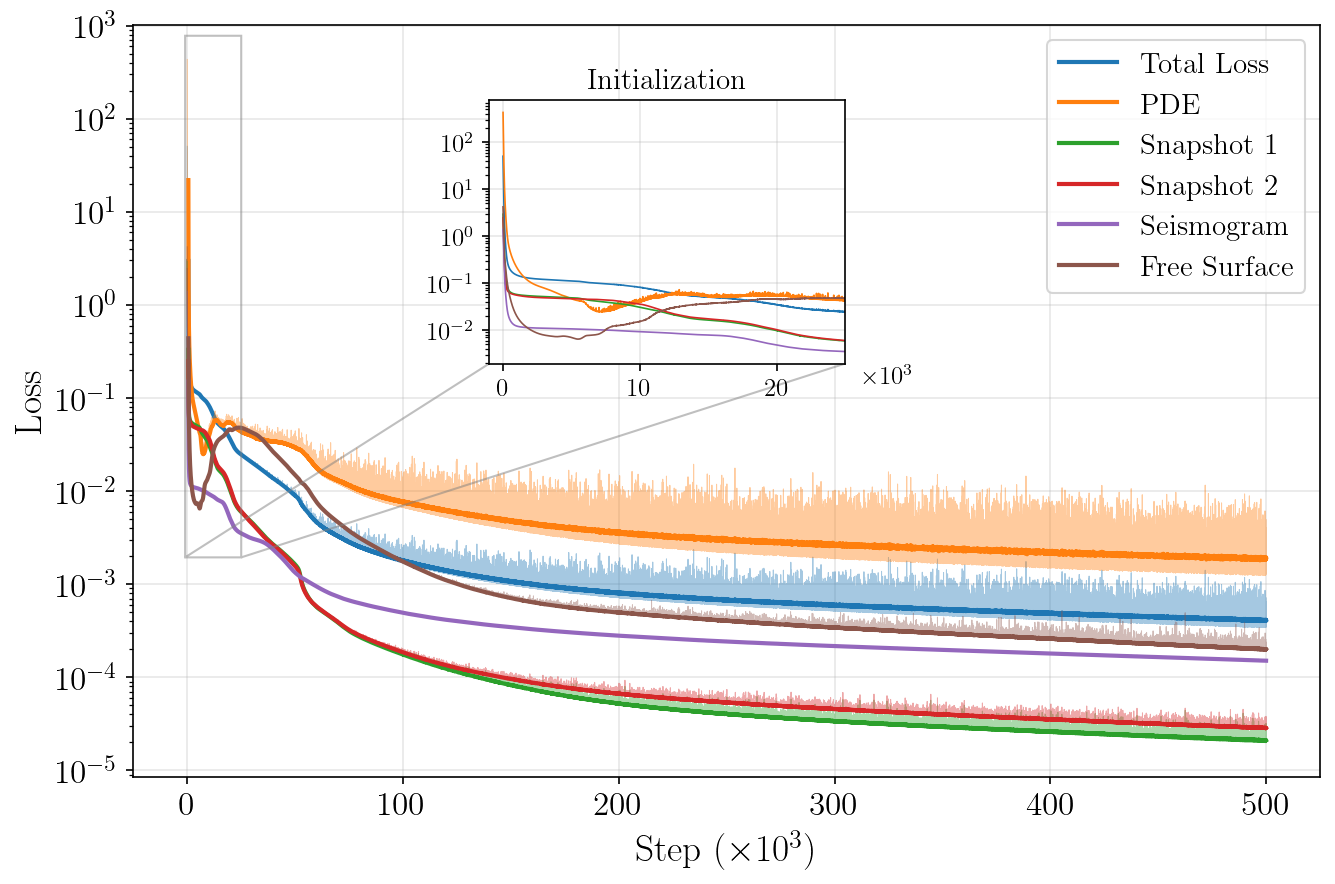
\includegraphics[width=\linewidth]{chapter5/metrics_losses.png}
\caption{Training loss decomposition for the classical FBPINN baseline on the anomaly benchmark: total loss, PDE residual, displacement-snapshot initial conditions (two components), seismogram misfit, and free-surface boundary condition, plotted versus training iteration. Inset: early-iteration behaviour showing rapid initial loss reduction.}
\label{fig:ch4-metrics-losses}
\end{figure}

\subsubsection{Network architectures and experimental setup}
\label{sec:ch4-results-setup}

To establish a rigorous comparison, we evaluate two distinct configurations applied to the identical FWI problem: a purely classical FBPINN baseline and our proposed hybrid quantum-classical architecture. In the classical baseline, both the decomposed wavefield network and the global velocity network are standard fully-connected networks with tanh activations. In the hybrid model, both are replaced by classical-to-quantum pipelines that terminate in four-qubit parameterized quantum circuits (PQCs).

Beyond the network heads, both configurations share the same FBPINN subdomain decomposition strategy ($5\!\times\!3\!\times\!5$ grid with a 0.35 overlap for the wavefield), the same use of a single global velocity network, and the same physics-informed composite loss function incorporating the PDE residual, wavefield snapshot initial conditions (ICs), data misfit, and free-surface boundary constraints. Notably, the quantum hybrid model achieves its expressivity using significantly fewer trainable parameters. We note that the two configurations are not matched parameter-for-parameter: the wavefield and velocity pre-networks differ in width and depth in addition to the quantum head (\ref{tab:ch4-hyperparams}), so the comparison reflects the combined classical-to-quantum substitution rather than the quantum circuit in isolation, and a parameter-matched classical control with the same backbone and a plain output head is not included here. Schematic representations of the hybrid framework (\ref{fig:ch4-hybrid-arch}) and the PQC topology (\ref{fig:ch4-pqc-architecture}) are provided alongside a summary of the network architectures in \ref{tab:ch4-hyperparams}. Methodological details, including the underlying acoustic wave equations and loss derivations, are detailed in the preceding subsections.

\subsection{Results}\label{sec:ch4-results}

We evaluate the proposed hybrid architecture on two wave-propagation benchmarks. The primary benchmark reconstructs a localized low-velocity anomaly from recordings acquired by a one-sided receiver array, providing a direct quantitative comparison between the quantum hybrid and a purely classical FBPINN baseline under matched FBPINN, loss, and optimizer settings. A second benchmark tests a checkerboard velocity pattern using the exact same network configuration, with only the collocation point density increased, to assess whether the proposed inversion framework can recover more spatially structured velocity variations without additional architectural tuning.

\subsubsection{Anomaly benchmark}
\label{sec:ch4-results-anomaly}

Our primary evaluation uses the velocity model established by Rasht-Behesht \emph{et al.}~\cite{rahst}, which defines a 2D acoustic domain ($1.15$\,km\,$\times$\,$0.45$\,km) featuring a localized low-velocity anomaly (approximately $2.5$\,km/s embedded within an approximately $3.0$\,km/s background; \ref{fig:ch4-anomaly}a). Ground-truth receiver data are generated by a spectral-element forward simulation~\cite{komatitsch1998spectral} driven by a Gaussian source at $(0.35,\,0.19)$\,km with dominant frequency $f_0 = 20$\,Hz. The inversion process is constrained by $500$\,ms of wavefield displacements recorded by a vertical array of 20 receivers positioned along the right boundary ($x = 1.15$\,km), supplemented by two early displacement snapshots ($t_0 = 0.100$\,s and $t_1 = 0.115$\,s). This transmission-dominated configuration, featuring a single source and a one-sided receiver array, represents a severely ill-posed inverse problem. The limited angular illumination inherently restricts the recovery of high-wavenumber spatial components, rigorously testing the regularizing capacity of the chosen neural architecture.

Starting from a purely homogeneous initial guess (\ref{fig:ch4-anomaly}b), both the classical and hybrid architectures successfully localize the low-velocity anomaly without suffering from the cycle-skipping artifacts that frequently plague classical adjoint-state FWI under poor starting models, which conventional FWI typically mitigates through multiscale or envelope-based strategies~\cite{11458622}. As illustrated by the inverted velocity field of the quantum hybrid model (\ref{fig:ch4-anomaly}c), the recovered anomaly closely tracks the true model's spatial distribution and peak amplitude. The minor lateral smearing observed in the reconstruction is consistent with the theoretical limits of resolving power imposed by the single-source geometry, confirming that the network has extracted the maximum available information from the receiver data.

The clearest distinction between the classical and quantum approaches emerges in their optimization dynamics. We quantify inversion accuracy by the L1 velocity error, the mean absolute difference between the inverted velocity field $\alpha$ and the true model $\alpha_\text{true}$ evaluated over an $N = 40\times40$ grid spanning the domain,
\begin{equation}
\mathrm{L1} = \frac{1}{N}\sum_{i=1}^{N}\bigl|\,\alpha(x_i,z_i) - \alpha_\text{true}(x_i,z_i)\,\bigr|,
\label{eq:ch4-l1}
\end{equation}
reported in km/s. \ref{fig:ch4-anomaly}d tracks the L1 velocity error against training iterations, revealing structurally different convergence trajectories. The quantum hybrid model undergoes a rapid initial descent, achieving an L1 error of $2.4\times 10^{-2}$ in merely $65{,}000$ iterations. By contrast, the classical baseline exhibits prolonged plateauing behavior, requiring $500{,}000$ iterations to reach a comparable, albeit slightly higher, final error of $2.9\times 10^{-2}$. This corresponds to an approximately $8\times$ reduction in the number of optimization iterations required to reach comparable or lower L1 velocity error, achieved despite the hybrid model using significantly fewer trainable parameters ($101{,}812$ vs.\ $151{,}836$). We emphasize that this comparison concerns optimization iterations rather than wall-clock runtime, since the per-iteration cost differs between the classical and hybrid architectures. We also note that the traces in \ref{fig:ch4-anomaly}d begin at different L1 errors: each model's velocity ($\alpha$) network initializes to a slightly different field about the homogeneous background, so the starting error reflects the random initialization of the differing $\alpha$-network architectures rather than any quantum effect (one classical velocity-network variant initializes to essentially the same L1 as the quantum hybrid). The comparison should accordingly be read as the iteration count needed to reach a given error, not as progress from a shared starting point.

\begin{figure}[!t]
\centering
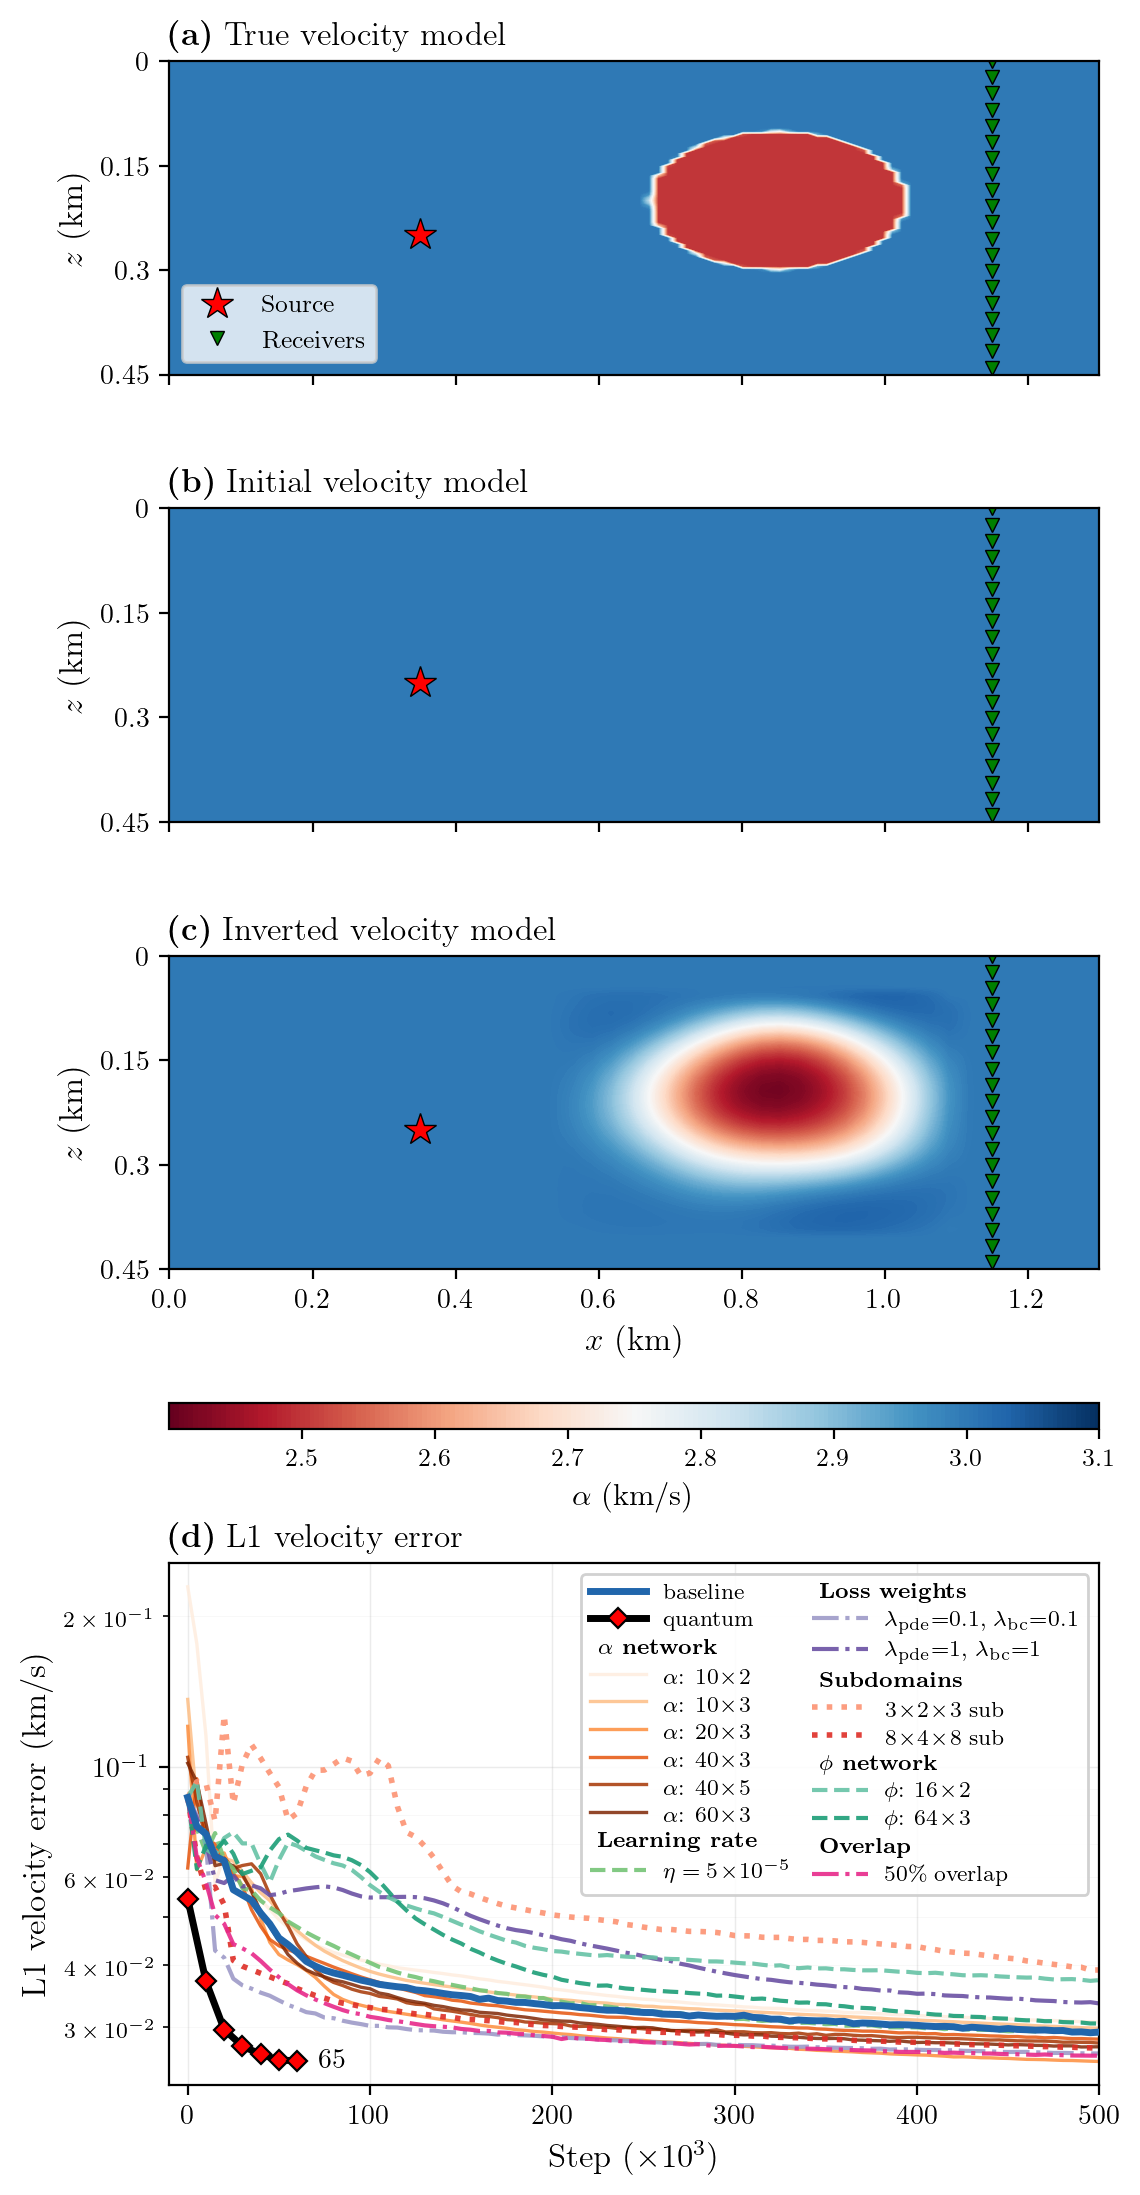
\includegraphics[width=\linewidth]{chapter5/l1_and_velocity.png}
\caption{Anomaly benchmark inversion and convergence. (a) True velocity model used for the spectral-element forward simulation, with source (red star) and receiver array (green triangles). (b) Initial homogeneous velocity model. (c) Inverted velocity model from the quantum hybrid FBPINN at $65{,}000$ training iterations. (d) L1 velocity error versus training iteration for the classical FBPINN baseline (blue), the quantum hybrid (red markers labeled 65k), and 14 of the 15 classical hyperparameter variants (thin colored lines). Traces begin at different initial L1 values because each velocity ($\alpha$) network initializes to a different (nominally homogeneous) field; this initial spread reflects initialization rather than training.}
\label{fig:ch4-anomaly}
\end{figure}

To test whether this performance gap could be explained by sub-optimal classical tuning, we conducted a systematic classical hyperparameter sweep comprising 15 distinct FBPINN variants. These baselines spanned a wide spectrum of configurations, including severely over-parameterized velocity networks (up to $60\!\times\!3$ hidden layers), alternative subdomain partitions ($3\!\times\!2\!\times\!3$ and $8\!\times\!4\!\times\!8$), varying learning rates, and adjusted physical loss weightings (detailed comprehensively in \ref{tab:ch4-hyperparams}). As depicted by the thin colored traces in \ref{fig:ch4-anomaly}d, simply increasing classical capacity or tuning hyperparameters failed to bridge the gap; none of the 15 classical configurations matched both the rapid early descent and the final L1 error achieved by the quantum hybrid within the tested training window ($500{,}000$ iterations).

\begin{table}[!t]
\centering
\caption{Network configurations and full hyperparameter sweep for the anomaly benchmark. The \texttt{classical} baseline (first row) and \texttt{quantum} hybrid (last row) are the two compared configurations; the intervening rows are the 15 classical hyperparameter variants. $\mathcal{Q}(n_q^{\times n_L})$ denotes a parameterized quantum circuit with $n_q$ qubits and $n_L$ layers. Values marked ``--'' are identical to the \texttt{classical} baseline. Subdomains column shows $\phi(\cdot)$ for wavefield decomposition.}
\label{tab:ch4-hyperparams}
\resizebox{\linewidth}{!}{%
\begin{tabular}{l l l c c c c c c c r}
\toprule
% \shortstack rather than \makecell: makecell nests a tabular, which the template
% rejects inside a table float ("Caption must be above table").
\textbf{Model} & \shortstack{$\boldsymbol{\phi}$ \textbf{network}\\$(x,z,t)\!\to\!\phi$} & \shortstack{$\boldsymbol{\alpha}$ \textbf{network}\\$(x,z)\!\to\!\alpha$} & \textbf{LR} & \textbf{Subs} & \textbf{Overlap} & $\boldsymbol{\lambda_\text{PDE}}$ & $\boldsymbol{\lambda_\text{IC}}$ & $\boldsymbol{\lambda_\text{data}}$ & $\boldsymbol{\lambda_\text{BC}}$ & \textbf{\# Pars} \\\midrule
\texttt{classical} & $\mathcal{N}$: $32^{\times2}\!\to\!16^{\times2}$ & $\mathcal{N}$: $20^{\times5}$ & $10^{-4}$ & $\phi(5\!\times\!3\!\times\!5)$ & 0.35 & 0.1 & 1.0 & 1.0 & 0.1 & 151{,}836 \\
\midrule
\multicolumn{11}{l}{\emph{$\phi$-network size variants}} \\
\texttt{phi16x2} & $\mathcal{N}$: $16^{\times2}$ & -- & -- & -- & -- & -- & -- & -- & -- & 25{,}836 \\
\texttt{phi64x3} & $\mathcal{N}$: $64^{\times3}$ & -- & -- & -- & -- & -- & -- & -- & -- & 649{,}836 \\
\midrule
\multicolumn{11}{l}{\emph{$\phi$ subdomain decomposition variants}} \\
\texttt{sub3x2x3} & -- & -- & -- & $\phi(3\!\times\!2\!\times\!3)$ & -- & -- & -- & -- & -- & 37{,}779 \\
\texttt{sub8x4x8} & -- & -- & -- & $\phi(8\!\times\!4\!\times\!8)$ & -- & -- & -- & -- & -- & 514{,}017 \\
\midrule
\multicolumn{11}{l}{\emph{$\alpha$-network size variants}} \\
\texttt{alpha10x2} & -- & $\mathcal{N}$: $10^{\times2}$ & -- & -- & -- & -- & -- & -- & -- & 150{,}226 \\
\texttt{alpha10x3} & -- & $\mathcal{N}$: $10^{\times3}$ & -- & -- & -- & -- & -- & -- & -- & 150{,}336 \\
\texttt{alpha20x3} & -- & $\mathcal{N}$: $20^{\times3}$ & -- & -- & -- & -- & -- & -- & -- & 150{,}996 \\
\texttt{alpha40x3} & -- & $\mathcal{N}$: $40^{\times3}$ & -- & -- & -- & -- & -- & -- & -- & 153{,}516 \\
\texttt{alpha40x5} & -- & $\mathcal{N}$: $40^{\times5}$ & -- & -- & -- & -- & -- & -- & -- & 156{,}796 \\
\texttt{alpha60x3} & -- & $\mathcal{N}$: $60^{\times3}$ & -- & -- & -- & -- & -- & -- & -- & 157{,}636 \\
\midrule
\multicolumn{11}{l}{\emph{Training hyperparameter variants}} \\
\texttt{lr5e4} & -- & -- & $5\!\times\!10^{-4}$ & -- & -- & -- & -- & -- & -- & -- \\
\texttt{lr5e5} & -- & -- & $5\!\times\!10^{-5}$ & -- & -- & -- & -- & -- & -- & -- \\
\texttt{overlap50} & -- & -- & -- & -- & 0.50 & -- & -- & -- & -- & -- \\
\texttt{wpde01\_wbc01} & -- & -- & -- & -- & -- & 0.01 & -- & -- & 0.01 & -- \\
\texttt{wpde1\_wbc1} & -- & -- & -- & -- & -- & 1.0 & -- & -- & 1.0 & -- \\
\midrule
\multicolumn{11}{l}{\emph{Quantum hybrid}} \\
\texttt{quantum} & $\mathcal{N}$: $32^{\times2}$ & $\mathcal{N}$: $20^{\times3}$ & -- & -- & -- & -- & -- & -- & -- & 101{,}812 \\
 & $\to$ $\mathcal{Q}$: $4^{\times2}$ & $\to$ $\mathcal{Q}$: $4^{\times2}$ & & & & & & & & \\
\bottomrule
\end{tabular}%
}
\end{table}

\subsubsection{Checkerboard benchmark}
\label{sec:ch4-results-checkerboard}

To further probe the resolution limits of the inversion pipeline, we test a checkerboard velocity model: a $3\times 3$ grid of alternating $\pm$$0.4$\,km/s perturbations on a $3.0$\,km/s background. The acquisition geometry is identical to the anomaly benchmark (same domain, source position, and receiver layout; \ref{fig:ch4-anomaly}a), as is the homogeneous initial model (\ref{fig:ch4-anomaly}b). The checkerboard forward simulation, however, uses a higher dominant source frequency, $f_0 = 60$\,Hz, compared with $f_0 = 20$\,Hz for the anomaly benchmark, so that the shorter wavelengths can resolve the finer spatial structure of the $3\times 3$ checkerboard. The checkerboard experiment thus tests recovery of higher spatial-frequency velocity structure under the same limited acquisition geometry.

Both the classical and quantum hybrid FBPINNs are run with the exact same network architectures and hyperparameters established for the anomaly benchmark (\ref{tab:ch4-hyperparams}). The training setup differs only in the use of a higher collocation point density, required to adequately constrain the smaller-scale spatial structures of the checkerboard pattern. Both models successfully resolve the checkerboard (\ref{fig:ch4-checkerboard}b). As expected from the single-source, one-sided receiver geometry, structural resolution degrades for blocks situated further from the receiver array. The successful inversion under this otherwise unchanged configuration confirms that the hybrid architecture generalizes beyond the anomaly benchmark without additional tuning.

\begin{figure}[!t]
\centering
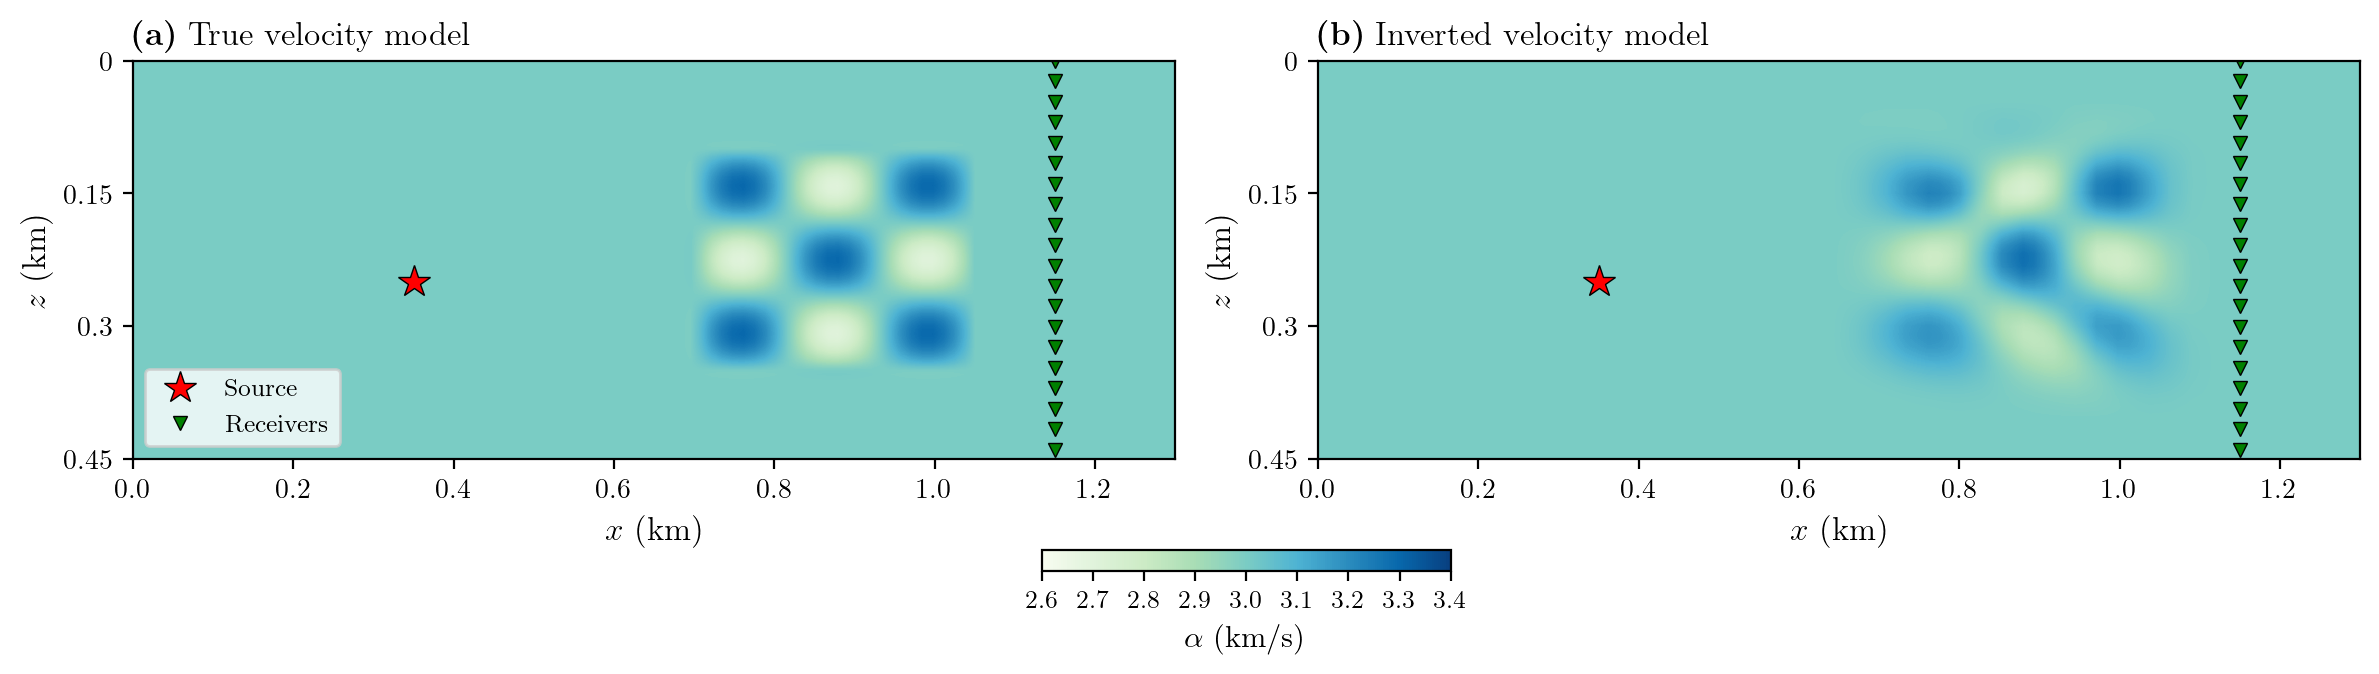
\includegraphics[width=\linewidth]{chapter5/true_and_inverted.png}
\caption{Checkerboard benchmark inversion. (a) True velocity model: a $3\times 3$ checkerboard of alternating $\pm$$0.4$\,km/s perturbations on a $3.0$\,km/s background, with source (red star) and receiver array (green triangles). (b) Inverted velocity model from the quantum hybrid FBPINN, using the identical network configuration from the anomaly benchmark with only the collocation point density increased.}
\label{fig:ch4-checkerboard}
\end{figure}

\subsection{Discussion}\label{sec:ch4-discussion}

The quantum hybrid's central result, a lower final L1 velocity error in approximately $8\times$ fewer training iterations with approximately $33$\% fewer trainable parameters, raises the question of what in the architecture produces it. We identify three contributing properties of the classical-to-PQC pipeline~\cite{cerezo2021variational}, while noting that our experiments do not isolate their individual effects.

First, the PQC is a parameter-efficient nonlinear map. Its output is governed by only $3nL+n$ trainable parameters, yet each enters through the joint action of non-commuting rotations rather than as an independent weight, so the same angles perform both feature mixing and output generation. This shared parameterization is consistent with the hybrid model matching or exceeding the classical baseline while using fewer parameters. We do not invoke the dimension of the underlying Hilbert space as a source of advantage: the measured output is a single bounded scalar, and for the circuits used here ($n=4$) it realizes only the low-order trigonometric family derived below.

Second, angle encoding endows the PQC output with a finite-frequency Fourier structure in the variables presented to the encoder. Because the PQC acts on the learned latent vector $\mathbf{z}(\mathbf{x}) = \mathcal{N}(\mathbf{x})$ rather than on the spatial coordinates directly, the relevant specialization of the result of Schuld \emph{et al.}~\cite{schuld2021effect} is
\begin{equation}
    f(\mathbf{x};\boldsymbol{\beta},\boldsymbol{\theta}_q) = \sum_{\boldsymbol{\omega}\in\Omega} c_{\boldsymbol{\omega}}(\boldsymbol{\theta}_q)\, e^{i\,\boldsymbol{\omega}\cdot(\boldsymbol{\beta}\odot\mathbf{z}(\mathbf{x}))},
\end{equation}
where the coefficients $c_{\boldsymbol{\omega}}$ are set by the trainable circuit angles and the accessible index set $\Omega$ is fixed by the encoding. For the $R_y(\beta_i z_i)$ encoding used here, each coordinate contributes only the indices $0,\pm 1$, so that for a single encoded variable
\begin{equation}
    f(s)=A+B\cos(\beta s)+C\sin(\beta s),
\end{equation}
with physical frequencies $0,\pm\beta_i$ that the trainable scales $\beta_i$ adapt during optimization; the derivation is given in Section~\ref{app:ch4-fourier}. This finite-frequency structure is not unique to quantum circuits: classical Fourier-feature mappings~\cite{tancik2020fourier}, and to a looser degree the nested sinusoidal activations of SIREN networks~\cite{sitzmann2020siren}, build the representation from a trigonometric basis and are an established remedy for the spectral bias of plain tanh networks. Relative to a fixed Fourier-feature layer with prescribed frequencies~\cite{tancik2020fourier}, the PQC differs in two respects: the encoding scales $\boldsymbol{\beta}$ are trainable, so the physical frequency grid adapts rather than being fixed a priori (a property it shares with SIREN, whose first-layer frequencies are likewise learned), and the entangling CNOT layers couple the per-coordinate features, populating cross-coordinate terms of $\Omega$ that an axis-aligned (additive) Fourier-feature layer does not produce on its own (an isotropic random Fourier mapping with a dense frequency matrix mixes coordinates and would). Two caveats temper this argument: the frequency bound applies to $f$ as a function of the learned latent $\mathbf{z}$ and not of the spatial coordinates, and our classical sweep contains only tanh architectures. A matched classical control with an explicit Fourier-feature or sinusoidal embedding is therefore the most informative comparison still missing, and we flag it as a priority below.

Third, the velocity output map hard-codes the range constraint $|\alpha-\alpha_\text{bg}|\leq A$. This bound is applied identically in both architectures, so it cannot by itself explain the gap; we note it only because, together with the bounded PQC output, it limits the latent signal entering the final map and may reduce large early-training excursions. Separately, the entangling CNOT layers provide a parameterization in which correlations among the latent variables are generated by the circuit dynamics rather than by stacked affine-plus-nonlinearity layers. Whether this yields a more favorable optimization trajectory, rather than a function class beyond the reach of a comparable MLP, is an empirical question we do not resolve here.

We stress that these properties bear mainly on representational capacity and parameter efficiency; none of them, on its own, predicts a faster convergence rate, so the link between the PQC parameterization and the observed iteration-count reduction remains to be established. The consistency of the improvement across the 15 classical hyperparameter variants (\ref{fig:ch4-anomaly}d) argues against the result being solely due to an unlucky baseline, though the models also begin from different initial L1 errors set by their velocity-network initializations. We emphasize, finally, that these gains are in optimization iterations on classically simulated circuits and do not constitute a quantum computational advantage; the simulated PQC realizes a function class that is, by construction, classically representable.

Our work complements recent hybrid quantum-PINN studies in other PDE-constrained settings. Leong \emph{et al.}~\cite{LEONG2025106782} benchmarked hybrid quantum PINNs for high-speed compressible flow, finding competitive accuracy at reduced parameter cost compared with classical PINNs. Berger \emph{et al.}~\cite{Berger2025} introduced trainable-embedding quantum PINNs for nonlinear PDEs including the Navier-Stokes equations, again observing efficiency gains at matched parameter count. The present work differs in two ways. First, we target a coupled forward-inverse problem (waveform inversion) rather than a pure forward PDE; the velocity field is learned jointly with the wavefield. Second, we integrate the PQC within a domain-decomposed FBPINN~\cite{Moseley2023}, extending the PINN-based FWI formulation of Rasht-Behesht \emph{et al.}~\cite{rahst} to handle larger and higher-frequency inversion problems via overlapping subdomain networks.

Several limitations should be noted: (i) The present experiments are two-dimensional acoustic and extending to three-dimensional elastic inversion, as pursued with classical physics-guided deep networks~\cite{10178066}, is the natural next step but is constrained by the $\mathcal{O}(2^n)$ memory cost of statevector simulation as qubit counts grow. Scaling to larger circuits on real hardware further raises the concern of barren plateaus (vanishingly small gradients in high-depth parameterized circuits~\cite{mcclean2018barren}), which would require careful initialization and ansatz choice. (ii) Inversions use a single source; production FWI pipelines incorporate a large number of sources with different illuminations, and PINN-based FWI in particular is known to be sensitive to loss-landscape pathologies under data sparsity~\cite{krishnapriyan2021failure}, which learned generative priors have been proposed to regularize~\cite{Wang2023diff}. (iii) The quantum circuit is simulated classically. On real NISQ hardware, gradients would be computed via the parameter-shift rule (two circuit evaluations per parameter), and device noise could erode the iteration-level advantage observed here.

Looking forward, the small qubit counts used here ($n=4$, $L=2$) are compatible with near-term quantum hardware, which suggests that genuine hardware demonstrations are feasible once noise-mitigation techniques reach sufficient maturity. Systematic studies at matched parameter counts across circuit depths and widths would clarify how the convergence advantage scales with quantum-circuit capacity. A matched classical control with an explicit Fourier-feature or sinusoidal embedding, added to the hyperparameter sweep, would in particular isolate how much of the observed advantage reflects the finite-frequency inductive bias rather than the quantum parameterization itself. Because the framework targets the general structure of physics-informed wave inversion rather than any geophysics-specific feature, we expect it to transfer directly to the broader wave-based inverse problems, such as medical ultrasound tomography, photoacoustic imaging, and non-destructive evaluation.

\subsection{Conclusion}

We introduced a hybrid quantum-classical FBPINN for acoustic FWI, in which the decomposed wavefield network and the global velocity network are represented by PQC-based classical-to-quantum pipelines within a domain-decomposed physics-informed framework, implemented as an end-to-end differentiable JAX program that avoids parameter-shift-rule overhead and jointly optimizes the classical PINN parameters and quantum circuit angles. On the anomaly benchmark, the hybrid model reaches a comparable or lower L1 velocity error in approximately $8\times$ fewer training iterations than the primary classical FBPINN baseline, despite using approximately $33$\% fewer trainable parameters, and it outperforms all 15 classical hyperparameter variants tested within the same $500{,}000$-iteration window. We emphasize that these gains are in optimization iteration count on classically simulated circuits and do not constitute a claim of quantum computational advantage, and that the mechanism behind the iteration-count reduction remains to be established. Key limitations include reliance on classical statevector simulation, a two-dimensional acoustic setup, a single-source configuration, and a comparison that is not parameter-matched and spans only tanh classical architectures. A matched classical control with an explicit Fourier-feature or sinusoidal embedding is the most informative experiment still needed. It would isolate how much of the advantage reflects a finite-frequency inductive bias rather than the quantum parameterization. Extension to elastic, three-dimensional, and multi-source inversion, and validation on near-term quantum hardware, are the natural next steps. Because the framework targets the general structure of physics-informed wave inversion rather than any geophysics-specific feature, we expect it to transfer to other wave-based inverse problems, such as medical ultrasound tomography and non-destructive evaluation.

\subsection{Data and Code Availability}

The data and code that support the findings of this study are available in the project repository at \url{https://github.com/x-repos/quFWI}.

\subsection{Appendix: Fourier Structure of the Angle-Encoded PQC}\label{app:ch4-fourier}

This note derives the finite-frequency structure of the PQC output used in the Discussion, specializing the general result of Schuld \emph{et al.}~\cite{schuld2021effect} to the angle encoding adopted in this work.

Consider first a single encoded scalar $s$ with Hermitian generator $G$ and encoding unitary $U_{\mathrm{enc}}(s)=e^{-i\beta s G}$, acting on the reference state $|\psi_0\rangle=|0\rangle^{\otimes n}$. Because the variational block $V(\boldsymbol{\theta}_q)$ is applied after the encoding, the averaged measurement observable $O=\frac{1}{n}\sum_{i=0}^{n-1}Z_i$ can be folded into the Heisenberg-picture operator $M(\boldsymbol{\theta}_q)=V(\boldsymbol{\theta}_q)^\dagger O\,V(\boldsymbol{\theta}_q)$, so the measured output is
\begin{equation}
  f(s)=\langle\psi_0|\,U_{\mathrm{enc}}(s)^\dagger M(\boldsymbol{\theta}_q)\,U_{\mathrm{enc}}(s)\,|\psi_0\rangle.
\end{equation}
Writing the spectral decomposition $G=\sum_a \lambda_a \Pi_a$ gives $U_{\mathrm{enc}}(s)=\sum_a e^{-i\beta s\lambda_a}\Pi_a$, and therefore
\begin{equation}
  f(s)=\sum_{a,b} e^{i\beta s(\lambda_a-\lambda_b)}\,\langle\psi_0|\,\Pi_a M(\boldsymbol{\theta}_q)\Pi_b\,|\psi_0\rangle,
\end{equation}
so the accessible frequency indices are the pairwise eigenvalue differences, $\Omega\subseteq\{\lambda_a-\lambda_b\}$. For the $R_y(\beta s)$ encoding used here, $G=Y/2$ has eigenvalues $\pm\tfrac{1}{2}$, so the differences are $0,\pm 1$ and
\begin{equation}
  f(s)=A+B\cos(\beta s)+C\sin(\beta s).
\end{equation}
The trainable angles change $A$, $B$, and $C$ but cannot create frequencies outside this set. This single-frequency (degree-one) spectrum is a consequence of encoding each variable exactly once: the $L$ variational layers act through the trainable parameters $\boldsymbol{\theta}_q$ and do not re-encode the data, so they enrich the coefficients but not the frequency set. Repeated (``data re-uploading'') encodings would extend the accessible spectrum to higher harmonics, but are not used here.

For the full register, each coordinate $z_i$ is encoded on its own qubit through $R_y(\beta_i z_i)$, so the encoding generators $\{Y_i/2\}$ act on disjoint tensor factors and mutually commute. The encoding unitary then factorizes as $\prod_i e^{-i\beta_i z_i Y_i/2}$, the per-coordinate spectra combine additively, and the accessible index set becomes $\Omega\subseteq\{-1,0,1\}^n$, with physical frequencies $\boldsymbol{\beta}\odot\boldsymbol{\omega}$. This is the multivariate Fourier form quoted in the Discussion. The entangling CNOT layers and variational angles determine which coefficients $c_{\boldsymbol{\omega}}$ are nonzero, in particular populating cross-coordinate indices, but they do not enlarge $\Omega$.

\subsection{Acknowledgment}

We thank the Reservoir Characterization Project (RCP), Colorado School of Mines, for financial support.

\input{chapter/06-conclusions}

% Example chapters (figures, tables, equations, journal papers) are in template/chapter/

% ><><><><><><><><><><><><><><><><><><><><><><><><><><><><><><><><><><><><><><><><
%                   BACK MATTER: Reference Cited
% ><><><><><><><><><><><><><><><><><><><><><><><><><><><><><><><><><><><><><><><><
\backmatter     % Leave this line here, it sets the formatting requirements for the back matter of the document

% >>>>>>>>> References Cited (required) <<<<<<<<<<
\urlstyle{rm}               % <-- Sets the URL font to be the same as the other text
\bibliography{supporting-files/thesis}

% >>>>>>>>> Selected Bibliography (optional) <<<<<<<<<<
\cleardoublepage
\begin{selected-bibliography}
<Your selected bibliography would go here, a page break might also be necessary above>
\end{selected-bibliography}

% Make sure the citations in you .bib file are correct. Especially double check that the resources type is correct. This will dictate how the items in the bibliography are formatted.
% We suggest using a citation management tool to create your .bib file. This make your references machine readable in the click of a button. Attend a Library workshop, visit the Library's website, or speak to a librarian about getting started with a citation management tool. This will make your life much easier. READ: MUCH EASIER! https://libguides.mines.edu/citing/software

% Look at http://bib-it.sourceforge.net/help/fieldsAndEntryTypes.php#phdthesis to find some information on the types of fields that exist. Also recommend using a reference manger. 


% >>>>>>>>> Appendices (if applicable) <<<<<<<<<<
% Appendices of the Chapter 3 paper (qawave-cpml)
% ======================================================================
% Appendix B: The convolutional PML in the Hamiltonian-simulation
% variables.  Self-contained fragment, \input from main.tex after the
% \appendix switch.  All labels are prefixed appB:.
% ======================================================================
\appendix{The convolutional PML in the Hamiltonian-simulation variables}
\label{ch3:appB:cpml}

This appendix expands the one-line statements of
Sections~\ref{ch3:sec:cpml}, \ref{ch3:sec:1d}, and \ref{ch3:sec:2d}: the causal kernel
and memory ODE from the CFS stretch
(Appendix~\ref{ch3:appB:kernel}), the one-dimensional memory generator and
the frequency-domain collapse (Appendix~\ref{ch3:appB:1d}), the proof that
the collapse is exact (Appendix~\ref{ch3:appB:collapse}), the
two-dimensional eight-block generator
(Appendix~\ref{ch3:appB:2d}), the staggered profile-sampling rule
(Appendix~\ref{ch3:appB:stagger}), and the profile formulas
(Appendix~\ref{ch3:appB:profiles}).  Throughout, $D$ is the
forward-difference matrix and $D^{\dagger}=-D_{\mathrm{b}}$ its negative
backward counterpart (Section~\ref{ch3:sec:wave}); all operators are exactly
those constructed in the accompanying code.

\subsection{From the CFS stretch to the memory ODE}
\label{ch3:appB:kernel}

We fix the Fourier convention
$\hat f(\omega)=\int dt\,e^{-i\omega t}f(t)$,
$f(t)=(2\pi)^{-1}\int d\omega\,e^{+i\omega t}\hat f(\omega)$, so that
$\partial_t\mapsto i\omega$ and the causal exponential has the transform
$\int_0^{\infty}dt\,e^{-\beta t}e^{-i\omega t}=(\beta+i\omega)^{-1}$ for
$\beta>0$.  A PML stretches the coordinate into the complex plane,
$\tilde x=\int_0^x s(x',\omega)\,dx'$, which in the frequency domain
replaces every spatial derivative by
$\partial_x\mapsto s(\omega)^{-1}\partial_x$ inside the layer.  For the
CFS factor of Eq.~\eqref{ch3:eq:cfs}, partial fractions in the variable
$i\omega$ give
\begin{equation}
  \frac{1}{s(\omega)}
  \;=\; \frac{\alpha+i\omega}{\kappa(\alpha+i\omega)+\sigma}
  \;=\; \frac{1}{\kappa} \;+\; \hat\zeta(\omega),
  \label{ch3:appB:eq:invs}
\end{equation}
with
\begin{equation}
  \hat\zeta(\omega) \;=\; -\frac{\sigma}{\kappa^{2}}\,
  \frac{1}{\beta+i\omega},
  \qquad
  \beta \;:=\; \frac{\sigma}{\kappa}+\alpha
  \label{ch3:appB:eq:zetahat}
\end{equation}
the CFS decay rate: indeed
$1/s-1/\kappa=(\kappa-s)/(\kappa s)$ with
$\kappa-s=-\sigma/(\alpha+i\omega)$ and
$\kappa s=\kappa^{2}(\beta+i\omega)/(\alpha+i\omega)$.  The single pole
at $i\omega=-\beta$ inverts, by the causal transform above, to the
exponential kernel of Eq.~\eqref{ch3:eq:kernel},
$\zeta(t)=-(\sigma/\kappa^{2})\,e^{-\beta t}\theta(t)$, and frequency
multiplication is time convolution:
$s^{-1}\partial_x f = \kappa^{-1}\partial_x f + \zeta * \partial_x f$.

The convolution becomes local in time once it is named.  Let
$\phi:=\zeta*\partial_x f$.  Multiplying Eq.~\eqref{ch3:appB:eq:invs} by
$(\beta+i\omega)$ gives the polynomial identity
$(\beta+i\omega)\hat\zeta=-\sigma/\kappa^{2}$, hence
$i\omega\,\hat\phi=-\beta\,\hat\phi
-(\sigma/\kappa^{2})\,\widehat{\partial_x f}$, which transforms back to
the memory ODE of Eq.~\eqref{ch3:eq:memoryode}.  Equivalently, in the time
domain,
$\partial_t\phi=\zeta(0^{+})\,\partial_x f+\zeta'*\partial_x f$ with
$\zeta(0^{+})=-\sigma/\kappa^{2}$ and $\zeta'=-\beta\zeta$.  One
first-order ODE per stretched derivative thus carries the convolution
exactly; this is the recursive-convolution CPML of Roden and
Gedney~\cite{roden2000cpml}.

\subsection{One dimension: memory generator and collapse}
\label{ch3:appB:1d}

In the variables of Section~\ref{ch3:sec:wave} the undamped 1D system is
$\dot v=-iDw$, $\dot w=-iD^{\dagger}v$ [Eq.~\eqref{ch3:eq:waveH}].  Each
equation contains exactly one spatial derivative, so the stretch
generates one memory field per physical field.  Sampling the profiles
per field (Appendix~\ref{ch3:appB:stagger}) defines the diagonal matrices
$\Sigma_v=\diag(\sigma_{v,j})$, $K_v=\diag(\kappa_{v,j})$,
$B_v=\diag(\sigma_{v,j}/\kappa_{v,j}+\alpha_{v,j})$, and the layer
projector $\Pi_v=\diag(\mathbf{1}[\sigma_{v,j}>0])$, and likewise for
$w$.  Applying the stretched-derivative rule to $-iDw$ and carrying the
convolution by the rescaled memory field
$\phi_v:=\gamma^{-1}\,\zeta_v*(-iDw)$---where $\gamma>0$ is a free
constant rescaling under which the physical trajectory is invariant,
set to the balanced value $\gamma=\sqrt{2\sigma_{\max}/h}$ of
Appendix~\ref{ch3:app:proof}---gives, by Eq.~\eqref{ch3:eq:memoryode},
\begin{equation}
  \dot v = -iK_v^{-1}Dw + \gamma\phi_v,
  \qquad
  \dot\phi_v = -B_v\phi_v + \frac{i}{\gamma}\Sigma_vK_v^{-2}Dw,
  \label{ch3:appB:eq:stretched}
\end{equation}
and the analogous pair for $(w,\phi_w)$ with $D\to D^{\dagger}$,
$v\leftrightarrow w$.  The source of $\phi_v$ carries the factor
$\Sigma_v$, so $\phi_v$ vanishes identically outside the layer strips
for memory-free data; masking the injection column by $\Pi_v$ therefore
changes no such trajectory while removing the spurious $O(\gamma)$
interior entries that an unmasked column would contribute to the
Hermitian part $H_1$.  On the four-block state
$[v;\,w;\,\phi_v;\,\phi_w]$ (two extra block qubits) the generator is
\begin{equation}
  A_{\mathrm{mem}} =
  \begin{bmatrix}
    0 & -iK_v^{-1}D & \gamma\Pi_v & 0\\[2pt]
    -iK_w^{-1}D^{\dagger} & 0 & 0 & \gamma\Pi_w\\[2pt]
    0 & \tfrac{i}{\gamma}\Sigma_vK_v^{-2}D & -B_v & 0\\[2pt]
    \tfrac{i}{\gamma}\Sigma_wK_w^{-2}D^{\dagger} & 0 & 0 & -B_w
  \end{bmatrix}.
  \label{ch3:appB:eq:gen1d}
\end{equation}

\emph{Collapse for $\kappa=1$, $\alpha=0$.}  In this case the stretch
degenerates: $s(\omega)=(i\omega+\sigma)/(i\omega)$, so the stretched
$v$ equation, $i\omega\hat v=s_v(\omega)^{-1}(-iD\hat w)$ per Fourier
mode, multiplies out to
\begin{equation}
  (i\omega+\sigma_v)\,\hat v \;=\; -iD\hat w,
  \label{ch3:appB:eq:freqcollapse}
\end{equation}
because the symbol $s(\omega)\,i\omega=i\omega+\sigma$ is a
\emph{first-degree polynomial} in $i\omega$.  Transforming back,
$\dot v=-iDw-\sigma_v v$, and likewise
$\dot w=-iD^{\dagger}v-\sigma_w w$: the convolution collapses to the
local damping of Eq.~\eqref{ch3:eq:1dcollapse},
$A=-iH-\diag(\sigma_v,\sigma_w)$, with no memory fields at all.

\subsection{Proof of the exact collapse}
\label{ch3:appB:collapse}

The frequency-domain argument above is formal (it commutes the stretch
with the time-domain initial-value problem); the following statement
makes the equivalence exact at the semi-discrete level.

\begin{lemma}[exact collapse]
\label{ch3:appB:lem:collapse}
Let $\kappa\equiv1$ and $\alpha\equiv0$ in the generator of
Eq.~\eqref{ch3:appB:eq:gen1d}, so that $B_v=\Sigma_v$ and
$B_w=\Sigma_w$, and define the defects
\begin{equation}
  e_v := \phi_v + \gamma^{-1}\Sigma_v v,
  \quad
  e_w := \phi_w + \gamma^{-1}\Sigma_w w.
  \label{ch3:appB:eq:defect}
\end{equation}
Then $\dot e_v=\dot e_w=0$ along every solution of
$\dot\Psi=A_{\mathrm{mem}}\Psi$.  Consequently a memory-form trajectory
projects onto a trajectory of the collapsed generator
Eq.~\eqref{ch3:eq:1dcollapse} if and only if $e_v(0)=e_w(0)=0$; for the
standard embedding $\phi_v(0)=\phi_w(0)=0$ this is the condition
$\Sigma_v v(0)=0$ and $\Sigma_w w(0)=0$, i.e.\ initial data supported
outside the layer.
\end{lemma}

\begin{lemproof}
Using both rows of Eq.~\eqref{ch3:appB:eq:stretched} with $B_v=\Sigma_v$,
\begin{equation*}
\begin{split}
  \dot e_v
  &= \Bigl[-\Sigma_v\phi_v+\tfrac{i}{\gamma}\Sigma_vDw\Bigr]
  + \gamma^{-1}\Sigma_v\bigl[-iDw+\gamma\Pi_v\phi_v\bigr]\\
  &= (\Sigma_v\Pi_v-\Sigma_v)\,\phi_v \;=\; 0,
\end{split}
\end{equation*}
since $\Sigma_v\Pi_v=\Sigma_v$ (the projector is the support indicator
of $\Sigma_v$); identically for $e_w$.  Equivalently, the block-row
operator
$E=\bigl[\begin{smallmatrix}
\gamma^{-1}\Sigma_v & 0 & I & 0\\
0 & \gamma^{-1}\Sigma_w & 0 & I
\end{smallmatrix}\bigr]$
annihilates the generator from the left, $EA_{\mathrm{mem}}=0$
(verified to round-off in our implementation).  On the invariant slice
$e\equiv0$ the memory ansatz $\phi_v=-\gamma^{-1}\Sigma_v v$ of
Section~\ref{ch3:sec:1d} holds at all times, the injection term becomes
$\gamma\Pi_v\phi_v=-\Sigma_v v$, and $(v,w)$ obeys
Eq.~\eqref{ch3:eq:1dcollapse}; conversely, every collapsed trajectory lifts
to the memory form through the ansatz.
\end{lemproof}

When $e(0)\neq0$, the conserved defect acts on the physical equations
as the static in-layer forcing $\gamma\Pi_ve_v(0)$,
$\gamma\Pi_we_w(0)$, so the discrepancy between the two forms scales
with the layer content $\lVert\Sigma_vv(0)\rVert$,
$\lVert\Sigma_ww(0)\rVert$ of the initial data---and vanishes exactly
for data supported outside the layer.  Numerically, propagating the
same interior pulse with Eq.~\eqref{ch3:appB:eq:gen1d} and with
Eq.~\eqref{ch3:eq:1dcollapse} agrees to $6\times10^{-13}$
(Section~\ref{ch3:sec:1d}).

\emph{Remark (the roles of $\alpha$ and $\kappa$).}  The cancellation
uses only $\alpha\equiv0$: for a graded $\kappa$ the modified defect
$e_v=\phi_v+\gamma^{-1}\Sigma_vK_v^{-1}v$ is conserved by the same
computation, and the convolution collapses to the local form
$\dot v=-iK_v^{-1}Dw-K_v^{-1}\Sigma_vv$ (both statements again verified
to round-off).  For $\alpha>0$, instead, $\dot e_v=-\diag(\alpha_v)\phi_v
\neq0$---equivalently, $s(\omega)\,i\omega$ is no longer polynomial in
$i\omega$---and the memory fields are irreducible: the four-block form
is then the genuine content of the CFS layer.

\subsection{Two dimensions: the eight-block generator}
\label{ch3:appB:2d}

In 2D the damping acts per direction: the $x$ stretch replaces every
$\partial_x$ and the $y$ stretch every $\partial_y$.  On the
separated-block state of Section~\ref{ch3:sec:wave} the undamped equations are
$\dot v=-iD_xw_x-iD_yw_y$, $\dot w_x=-iD_x^{\dagger}v$,
$\dot w_y=-iD_y^{\dagger}v$, with $D_x=D\otimes I_{N_y}$ and
$D_y=I_{N_x}\otimes D$ on the flattened $N_xN_y$ grid register ($x$
register more significant).  The $v$ equation contains one derivative
of each direction and acquires two memory fields $\phi_{vx}$,
$\phi_{vy}$; each $w$ equation contains a single derivative and
acquires one, $\phi_x$ for $w_x$ and $\phi_y$ for $w_y$.  The four
memory fields plus the three physical fields are padded by one zero
block to the eight blocks of Eq.~\eqref{ch3:eq:blocks} (three block
qubits).

Because $\sigma_x$ depends on $x$ only, its diagonal samples factorise
on the grid register:
$\Sigma_v^{x}=S_x\otimes I_{N_y}$ and
$\Sigma_w^{x}=S_x^{\mathrm{st}}\otimes I_{N_y}$, where
$S_x=\diag\,\sigma(x_j)$ holds the nodal samples and
$S_x^{\mathrm{st}}=\diag\,\sigma(x_{j-1/2})$ the half-cell samples
(Appendix~\ref{ch3:appB:stagger}); symmetrically
$\Sigma_v^{y}=I_{N_x}\otimes S_y$ and
$\Sigma_w^{y}=I_{N_x}\otimes S_y^{\mathrm{st}}$.  With $\kappa\equiv1$
(our 2D configurations), the decay rates are
$B_v^{x}=\Sigma_v^{x}+\diag\alpha_x(x_j)$ etc., and the masks
$\Pi_v^{x}=\diag(\mathbf{1}[\Sigma_v^{x}>0])$, \dots\ are the
layer-strip projectors.  Repeating the derivation of
Appendix~\ref{ch3:appB:1d} once per (field, stretched direction) pair gives
the generator, in the block ordering of Eq.~\eqref{ch3:eq:blocks},
\begin{widetext}
\begin{equation}
  A \;=\;
  \begin{bmatrix}
    0 & -iD_x & -iD_y & \gamma\Pi_v^{x} & \gamma\Pi_v^{y} & 0 & 0 & 0\\[3pt]
    -iD_x^{\dagger} & 0 & 0 & 0 & 0 & \gamma\Pi_w^{x} & 0 & 0\\[3pt]
    -iD_y^{\dagger} & 0 & 0 & 0 & 0 & 0 & \gamma\Pi_w^{y} & 0\\[3pt]
    0 & \frac{i}{\gamma}\Sigma_v^{x}D_x & 0 & -B_v^{x} & 0 & 0 & 0 & 0\\[3pt]
    0 & 0 & \frac{i}{\gamma}\Sigma_v^{y}D_y & 0 & -B_v^{y} & 0 & 0 & 0\\[3pt]
    \frac{i}{\gamma}\Sigma_w^{x}D_x^{\dagger} & 0 & 0 & 0 & 0 & -B_w^{x} & 0 & 0\\[3pt]
    \frac{i}{\gamma}\Sigma_w^{y}D_y^{\dagger} & 0 & 0 & 0 & 0 & 0 & -B_w^{y} & 0\\[3pt]
    0 & 0 & 0 & 0 & 0 & 0 & 0 & 0
  \end{bmatrix}
  \quad\text{on}\quad
  \bigl[\,v;\; w_x;\; w_y;\; \phi_{vx};\; \phi_{vy};\;
        \phi_{x};\; \phi_{y};\; 0\,\bigr],
  \label{ch3:appB:eq:gen2d}
\end{equation}
\end{widetext}
which is, entry for entry, the matrix assembled by the accompanying
implementation.

\emph{Strip masking.}  The source of each memory field carries its own
profile factor ($\Sigma_v^{x}$ for $\phi_{vx}$, \dots), so the field
remains identically zero outside its layer strip for memory-free
initial data; the corresponding injection column is masked by the strip
projector, exactly as in 1D, so that $H_1$ carries no spurious
interior coupling.

\emph{Corners.}  In a corner cell both $\sigma_x>0$ and $\sigma_y>0$
hold simultaneously: both directions' memory fields are active there,
the same generator entries of Eq.~\eqref{ch3:appB:eq:gen2d} apply
unchanged, and no corner-specific terms arise.  This is the structural
advantage of the unsplit convolutional PML over split-field
formulations~\cite{roden2000cpml}.  The measured stability,
$\max\operatorname{Re}\operatorname{eig}(A)=0$ to round-off, is
reported in Section~\ref{ch3:sec:2d}.

\subsection{The staggered sampling rule}
\label{ch3:appB:stagger}

For the forward-difference convention, $(Dw)_j=(w_{j+1}-w_j)/h$.  The
component $v_j$ is updated through $(Dw)_j$ and represents the field at
the integer node $x_j=jh$; the component $w_j$ is updated through
$(D^{\dagger}v)_j\propto v_j-v_{j-1}$, a difference centered at the
half-cell point $x_{j-1/2}$, so the $w$ field lives on the staggered
grid (the backward convention shifts it to $x_{j+1/2}$).  The sampling
rule follows: \emph{every profile factor in an evolution equation is
sampled on the grid of the field that the equation updates},
\begin{equation}
  \sigma_{v,j}=\sigma(x_j),
  \qquad
  \sigma_{w,j}=\sigma(x_{j\mp1/2}),
  \label{ch3:appB:eq:staggerrule}
\end{equation}
with the upper (lower) sign for the forward (backward) convention,
and per direction in 2D (\ref{ch3:appB:tab:stagger}): only the $x$
profile of the $w_x$ family and the $y$ profile of the $w_y$ family are
staggered; all other dependencies are nodal.

\begin{table}
\caption{Staggered sampling of the damping profiles in 2D
(forward-difference convention; the backward convention flips the
half-cell shifts).  Each profile is sampled on the grid of the field
its equation updates.}
\label{ch3:appB:tab:stagger}
\begin{tabular}{lll}
\toprule
Field & Lives at & Profile samples \\
\midrule
$v$   & $(x_j,\,y_k)$         & $\sigma(x_j)$,\ $\sigma(y_k)$ \\
$w_x$ & $(x_{j-1/2},\,y_k)$   & $\sigma(x_{j-1/2})$ \\
$w_y$ & $(x_j,\,y_{k-1/2})$   & $\sigma(y_{k-1/2})$ \\
\bottomrule
\end{tabular}
\end{table}

\emph{Ablation.}  Sampling all profiles at the integer nodes
instead---the only change being the half-cell shift of the $w$
profiles---degrades the measured gold-standard reflection of
Section~\ref{ch3:sec:2d} by factors of 120--235.  At the reflection floors of
\ref{ch3:fig:convergence}(a,b) the half-cell stagger is load-bearing,
not a refinement.

\subsection{Profile formulas}
\label{ch3:appB:profiles}

Within a layer of $n_{\mathrm{pml}}$ points (width
$L=n_{\mathrm{pml}}h$) the damping is polynomially graded in the depth
$d$ measured from the interface,
\begin{equation}
  \sigma(d) \;=\; \sigma_{\max}\,(d/L)^{m},
  \qquad 0\le d\le L,
  \label{ch3:appB:eq:sigma}
\end{equation}
and zero outside; the interface node itself is undamped,
$\sigma(0)=0$, the outermost node attains $\sigma_{\max}$, and
staggered samples beyond the wall are clipped to $d=L$.  The amplitude
follows from the normal-incidence round trip: a wave crossing the
layer, reflecting off the terminating hard wall, and crossing back
accumulates the attenuation
\begin{equation}
  R \;=\; \exp\Bigl[-\frac{2}{c}\int_0^{L}\sigma(x)\,dx\Bigr]
  \;=\; \exp\Bigl[-\frac{2\,\sigma_{\max}L}{(m+1)\,c}\Bigr],
  \label{ch3:appB:eq:roundtrip}
\end{equation}
so prescribing a design reflection $R_0$ gives the Collino--Tsogka
amplitude~\cite{collino2001pml}
\begin{equation}
  \sigma_{\max} \;=\; -\frac{(m+1)\,c\,\ln R_0}{2L},
  \label{ch3:appB:eq:sigmamax}
\end{equation}
used with the standard recipe $m=2$,
$R_0=10^{-3}$~\cite{komatitsch2007unsplit}.  The nominal $R_0$ is
realised only for layers of ${\gtrsim}8$ points; for thinner layers the
discrete transition error dominates (a four-point layer reflects at the
$0.5$--$2\%$ level for grid-scale wavelengths), consistent with the
saturation of \ref{ch3:fig:convergence}(a).

When the CFS parameters are used they are graded with the same
geometry,
\begin{equation}
  \kappa(d) = 1 + (\kappa_{\max}-1)\,(d/L)^{m},
  \quad
  \alpha(d) = \alpha_{\max}\,(1-d/L),
  \label{ch3:appB:eq:grading}
\end{equation}
$\kappa$ rising from $1$ at the interface to $\kappa_{\max}$ at the
wall with the same polynomial as $\sigma$, and $\alpha$ tapering
linearly~\cite{komatitsch2007unsplit} from $\alpha_{\max}$ just inside
the interface to zero at the wall (and vanishing identically outside
the layer); in the implementation
$\alpha(d)=\alpha_{\max}[1-(\sigma(d)/\sigma_{\max})^{1/m}]$, which is
identical.  A nonzero $\alpha$ improves grazing-incidence and
evanescent absorption but unmatches the layer at low frequencies (the
stretch is matched only for $\omega\gg\alpha$), so the fixed-horizon
absorption benchmarks of Section~\ref{ch3:sec:2d} use $\alpha_{\max}=0$.
Finally, the memory rescaling defaults to
$\gamma=\sqrt{2\sigma_{\max}/h}$, the choice that balances the
injection and memory-source contributions to $\lamax(H_1)$
(Appendix~\ref{ch3:app:proof}).

% ======================================================================
% Appendix C: Schrodingerisation -- discrete formulas and recovery.
% Fragment; \input into main.tex.  All labels prefixed appC:.
% ======================================================================
\appendix{Schr\"odingerisation: discrete formulas and recovery}
\label{ch3:appC:schro}

This appendix records the complete discrete recipe behind the summary of
Section~\ref{ch3:sec:schro}, with the exact sign, grid, and ordering conventions
of our implementation; these are the conventions validated end to end by
the demonstrations of Section~\ref{ch3:sec:demos}.

\subsection{Hermitian split and warped transform}
\label{ch3:appC:transform}

The semi-discrete absorbing dynamics $\dot z = Az$ is split as
\begin{equation}
  A = H_1 + iH_2, \qquad
  H_1 = \frac{A + A^{\dagger}}{2}, \qquad
  H_2 = \frac{A - A^{\dagger}}{2i},
  \label{ch3:appC:split}
\end{equation}
with the dissipative part $H_1$ and the Hamiltonian part $H_2$ both
Hermitian.  The warped phase-space transform of
Ref.~\cite{jin2023schrodingerisation} appends one auxiliary variable $p$
and sets $w(t,p) = e^{-p}z(t)$ for $p\ge0$ (extended to $p<0$ by the
profile $g$ of Section~\ref{ch3:appC:initial}).  The sign structure follows in
one line: along the exact solution, $\partial_t w = e^{-p}Az = Aw$ and
$\partial_p w = -e^{-p}z = -w$, so $H_1 w = -H_1\,\partial_p w$ and
\begin{equation}
  \partial_t w \;=\; -H_1\,\partial_p w \;+\; iH_2\,w,
  \label{ch3:appC:warped}
\end{equation}
a transport equation in $p$: the non-unitary part of $A$ has become
advection of the auxiliary variable.

\subsection{Discrete setup and per-mode evolution}
\label{ch3:appC:discrete}

The $p$ register holds $N_p = 2^{n_p}$ grid points on the periodic domain
$[-p_{\max},\,p_{\max})$,
\begin{equation}
  p_j = -p_{\max} + j\,\Delta p, \qquad
  \Delta p = \frac{2p_{\max}}{N_p},
  \label{ch3:appC:grid}
\end{equation}
$j = 0,\dots,N_p-1$, with dual frequencies $\eta_k = \pi k/p_{\max}$ for
$k = -N_p/2,\dots,N_p/2-1$ in FFT ordering [i.e.\
$\eta = 2\pi\times\texttt{fftfreq}(N_p,\Delta p)$].  We fix the Fourier
\emph{synthesis} convention $w(\cdot,p) = \sum_k \hat w_k\,e^{+i\eta_k p}$
(NumPy: $w = \mathrm{ifft}(\hat w)$ along the $p$ axis,
$\hat w = \mathrm{fft}(w)$).  Substituting
$\partial_p \to i\eta_k$ in Eq.~\eqref{ch3:appC:warped} decouples the modes
into the unitary evolutions of Eq.~\eqref{ch3:eq:permode},
\begin{equation}
\begin{split}
  \frac{d\hat w_k}{dt} &= -i\,(\eta_k H_1 - H_2)\,\hat w_k \\
  \Longrightarrow\quad
  \hat w_k(T) &= e^{-iT(\eta_k H_1 - H_2)}\,\hat w_k(0).
\end{split}
  \label{ch3:appC:permode}
\end{equation}
Stacking the modes, the whole evolution is one Hamiltonian simulation,
\begin{equation}
  H_{\mathrm{tot}} \;=\; D_\eta \otimes H_1 \;-\; I_p \otimes H_2,
  \qquad D_\eta = \diag(\eta_k),
  \label{ch3:appC:htot}
\end{equation}
acting on the tensor order ($p$ register, system register) with the $p$
register most significant: on the circuit, qubits $0,\dots,n_s-1$ carry
the system register (little-endian) and qubits $n_s,\dots,n_s+n_p-1$ the
$p$ register, so the flattened statevector index is $j\,2^{n_s} + s$.
The opening $\mathrm{QFT}^{\dagger}$ on the $p$ register maps the grid
amplitudes to $\hat w/\sqrt{N_p}$ (the unitarily normalised FFT),
$e^{-iTH_{\mathrm{tot}}}$ acts in the $\eta$ basis, and the closing
$\mathrm{QFT}$ returns to the $p$ grid [\ref{ch3:fig:circuits}(b)].

\subsection{Initial data and the $C^{1}$ profile}
\label{ch3:appC:initial}

The initial condition $w(0,p_j) = g(p_j)\,z(0)$ is a product state across
the two registers,
\begin{equation}
  \lvert W(0)\rangle
  = \frac{\lvert g\rangle \otimes \lvert z_0\rangle}{N_0},
  \qquad
  N_0 = \lVert g\rVert_2\,\lVert z_0\rVert_2,
  \label{ch3:appC:product}
\end{equation}
with the normalisation $N_0$ recorded classically and undone at recovery.
The plain profile $g(p) = e^{-\lvert p\rvert}$ is kinked at $p=0$ and
limits the $p$ discretisation to $O(\Delta p)$; the $C^{1}$ cubic of
Ref.~\cite[Remark~4.9]{jin2024recovery} replaces it on $(-1,0)$,
\begin{equation}
  g(p) =
  \begin{cases}
    e^{-p}, & p \ge 0,\\[3pt]
    \Bigl(\dfrac{3}{e}-3\Bigr)p^{3}
      + \Bigl(\dfrac{4}{e}-5\Bigr)p^{2} - p + 1, & -1 < p < 0,\\[7pt]
    e^{p}, & p \le -1,
  \end{cases}
  \label{ch3:appC:profile}
\end{equation}
restoring $O(\Delta p^{2})$.  The junctions are $C^{1}$ by construction:
at $p=0^{-}$ the cubic gives $g=1$, $g'=-1$, matching $e^{-p}$; at
$p=-1^{+}$ it gives $g = g' = e^{-1}$, matching $e^{p}$.  Because
$g(p) = e^{-p}$ \emph{exactly} for $p\ge0$, the recovery formula below is
unchanged by the smoothing.  Measured on the 1D CPML benchmark of
\ref{ch3:fig:convergence}(c) ($2^{5}$ spatial points,
$n_{\mathrm{pml}}=8$, $\sigma_{\max}=1$, $T=30$, $p_{\max}=18$): the
recovery error at the default slice falls from $4.1\times10^{-2}$ to
$6.3\times10^{-4}$ over $n_p = 6$--$11$ for the kinked profile and from
$1.3\times10^{-2}$ to $2.4\times10^{-6}$ for the cubic, with fitted
slopes of $\log_2(\mathrm{error})$ versus $n_p$ of $-1.2$ and $-2.6$
($-1.6$ and $-3.4$ on the pre-floor points $n_p\le9$)---at or above the
nominal first- and second-order rates, confirming the one-order upgrade
of Ref.~\cite{jin2024recovery} in this setting.

\subsection{Recovery: threshold, wraparound, plateau}
\label{ch3:appC:recovery}

The solution is recovered from a single grid slice,
\begin{equation}
  z(T) \;=\; e^{p^{*}}\,w(T,p^{*}),
  \qquad
  p^{*} \;\ge\; \lamax^{+}(H_1)\,T,
  \label{ch3:appC:recover}
\end{equation}
where $\lamax^{+} = \max\{0,\lamax(H_1)\}$ and the validity threshold on
$p^{*}$ is Theorem~3.1 of Ref.~\cite{jin2024recovery}.  When
$H_1\preceq0$ (the collapsed 1D CPML and the sponge) any $p^{*}>0$ is
admissible, and the implementation defaults to the slice three grid
points above $p=0$, i.e.\ $p^{*} = 3\Delta p$.  For indefinite $H_1$ (the
2D CPML memory form of Lemma~\ref{ch3:lem:threshold}) the slice must be
placed explicitly at $p^{*}\ge\lambda^{+}T$; below the threshold the
recovered state is $O(1)$ wrong (\ref{ch3:fig:threshold}).

Two further discrete conditions guard the slice.  \emph{Wraparound}: in
Eq.~\eqref{ch3:appC:warped} an $H_1$-eigencomponent with eigenvalue $\lambda$
is advected in $p$ with velocity $\lambda$, so the most strongly damped
components travel a distance $\lambda^{-}T$ \emph{leftwards}, with
$\lambda^{-} = \lvert\lambda_{\min}(H_1)\rvert$ ($=\sigma_{\max}$ for the
diagonal absorbers).  The discrete $p$ domain is periodic, so
$p_{\max}$ must be wide enough that this leftward-transported mass does
not wrap through $p=-p_{\max}$ back into the recovery region.
\emph{Plateau}: since $e^{p}w(T,p) = z(T)$ for every admissible $p$, the
function $p\mapsto e^{p}\lVert w(T,p)\rVert$ must be flat across the
recovery window.  The implementation tabulates it over the first twelve
grid points right of $p=0$ and reports the relative peak-to-peak spread;
a flat plateau certifies that $p_{\max}$, $N_p$, and the profile are
adequate (our regression tests require a spread below $5\times10^{-2}$),
while a tilted or stepped plateau flags wraparound or an under-resolved
profile.

\subsection{Measurement interpretation}
\label{ch3:appC:measure}

The pipeline is unitary, so the final statevector is exactly
$W(T)/N_0$, holding $w_s(T,p_j)/N_0$ at index $j\,2^{n_s}+s$.  Measuring
the $p$ register returns outcome $p_j$ with probability
$\lVert w(T,p_j)\rVert^{2}/N_0^{2}$ and collapses the system register
onto $w(T,p_j)/\lVert w(T,p_j)\rVert = z(T)/\lVert z(T)\rVert$: every
slice in the admissible window yields the \emph{same} normalised state,
so post-selection may accept the whole plateau window rather than a
single outcome, summing the corresponding probabilities.  The success
probability of the slice at $p^{*}$ is, up to $p$-discretisation error,
\begin{equation}
  \Pr(p^{*})
  \;=\; \frac{e^{-2p^{*}}\,\lVert z(T)\rVert^{2}}{N_0^{2}}
  \;\propto\; e^{-2p^{*}},
  \label{ch3:appC:psuccess}
\end{equation}
which at the threshold slice $p^{*} = \lambda^{+}T$ is the
$e^{-2\lambda^{+}T}$ post-selection penalty of Section~\ref{ch3:sec:lemma}---the
cost that the Lyapunov symmetrizer of Section~\ref{ch3:sec:symmetrizer} replaces
by the $T$-independent factor $\kappa_2^{2}(S)$.  On the statevector
simulator used for the demonstrations of Section~\ref{ch3:sec:demos}, the slice
is read off rather than sampled: the final statevector is reshaped to an
$N_p\times2^{n_s}$ array, row $j$ at $p^{*}$ is extracted, and the result
is rescaled by $e^{p_j}N_0$.  This is deterministic and exact, so the
reported errors measure the Trotter and discretisation error only; on
hardware the same slice would additionally cost the factor
$e^{-2p^{*}}$ of Eq.~\eqref{ch3:appC:psuccess} in repetitions.

% ----------------------------------------------------------------------
% Appendix D: validation protocol and convergence data.
% Fragment to be \input into main.tex after \appendix.
% All numbers from paper/experiments/convergence_results.json and
% paper/draft.md; the stagger ablation reproduced from the library
% (lib/absorbing.py) under the same gold-standard protocol.
% ----------------------------------------------------------------------

\appendix{Validation protocol and convergence data}
\label{ch3:appD:validation}

This appendix records the classical validation protocol behind every
reflection number quoted in Section~\ref{ch3:sec:2d} and the raw convergence
data behind the fitted orders of Section~\ref{ch3:sec:circuit}
[\ref{ch3:fig:convergence}(a--d)].

\subsection{Gold-standard reflection protocol}
\label{ch3:appD:protocol}

Measuring the residual reflection of an absorbing layer against the
absorbing dynamics itself is circular; the gold standard is the
open-domain solution.  The truncated domain has $N=128$ points (seven
grid qubits) with the CPML occupying $n_{\mathrm{pml}}$ points at each
end.  The initial data are a Gaussian velocity bump centred at $j=64$
with width $3$ cells and $w(0)=0$, normalised to
$\lVert z_0\rVert_2=1$.  The reference embeds the \emph{same} truncated
data centred in a $4\times$ hard-wall domain ($N_{\mathrm{ref}}=512$,
embedding offset $\Delta=(N_{\mathrm{ref}}-N)/2=192$) and evolves it
with the closed-domain unitary $e^{-iH_{\mathrm{ref}}T}$.  Both
evolutions are computed by dense matrix exponentials, so the comparison
contains no time-integration error.  The reported error is the
pointwise $\ell_2$ difference on the interior window,
\begin{equation}
  E(T)^{2} \;=\; \sum_{f\in\{v,\,w\}}\;
  \sum_{j=n_{\mathrm{pml}}}^{N-n_{\mathrm{pml}}-1}
  \bigl|\, f_j(T) - f^{\mathrm{ref}}_{j+\Delta}(T) \,\bigr|^{2}.
  \label{ch3:appD:eq:gold}
\end{equation}
Two checks make the protocol sound.  (i)~\emph{Window alignment}: at
$T=0$ the windowed difference in Eq.~\eqref{ch3:appD:eq:gold} evaluates to
exactly zero in floating point, pinning the embedding offset and the
index conventions.  (ii)~\emph{Causal validity}: with $c=1$, $h=1$ the
pulse meets the layer interface at depth $j=n_{\mathrm{pml}}$ and its
reflection is back at the centre by
$T\approx2(64-n_{\mathrm{pml}})\le120$ for $n_{\mathrm{pml}}\ge4$,
whereas the far walls of the reference domain are first felt inside the
comparison window only at $T\approx380$.  The plateau times
$T\in\{100,120,140\}$ therefore capture the complete round-trip
reflection of the truncated domain while the reference is still
uncontaminated.  The reported reflection is the maximum of $E(T)$ over
the three plateau times, and the relative plateau spread
[$(\max-\min)/\mathrm{mean}$] is the flatness diagnostic.  A reduced
instance of the same protocol ($N=64$ versus $256$, $T=20$ and $60$,
asserted $<10^{-3}$) is pinned in the unit-test suite
(Section~\ref{ch3:appD:tests}).

\subsection{Reflection versus layer width and design reflection}
\label{ch3:appD:reflection}

\begin{table}
\caption{Gold-standard true reflection (1D CPML, $N=128$ versus the
$N=512$ hard-wall reference, $m=2$): plateau error
$\max_{T\in\{100,120,140\}}E(T)$ and relative plateau spread.  Upper
block: layer-width sweep at $R_0=10^{-3}$; lower block: design-reflection
sweep at $n_{\mathrm{pml}}=12$.}
\label{ch3:appD:tab:reflection}
\begin{tabular}{llll}
\toprule
$n_{\mathrm{pml}}$ & $R_0$ & plateau error & plateau spread \\
\midrule
4  & $10^{-3}$ & $6.7\times10^{-4}$ & $1.0\times10^{-9}$ \\
6  & $10^{-3}$ & $2.6\times10^{-4}$ & $3.3\times10^{-10}$ \\
8  & $10^{-3}$ & $2.6\times10^{-4}$ & $2.2\times10^{-10}$ \\
12 & $10^{-3}$ & $3.4\times10^{-4}$ & $1.7\times10^{-9}$ \\
16 & $10^{-3}$ & $4.2\times10^{-4}$ & $3.3\times10^{-5}$ \\
\midrule
12 & $10^{-2}$ & $4.5\times10^{-3}$ & $1.5\times10^{-10}$ \\
12 & $10^{-3}$ & $3.4\times10^{-4}$ & $1.7\times10^{-9}$ \\
12 & $10^{-4}$ & $4.3\times10^{-5}$ & $1.9\times10^{-7}$ \\
\bottomrule
\end{tabular}
\end{table}

\ref{ch3:appD:tab:reflection} interprets as follows.  The curve is
the sum of two competing contributions.  At the thinnest layer
($n_{\mathrm{pml}}=4$) the discrete transition error dominates: the
measured reflection sits $9.4\times$ above the discrete wall-return
prediction.  For $n_{\mathrm{pml}}\ge8$ the transition error is
negligible and the reflection is set by the wall return, which
\emph{rises toward the design value from below} as the layer widens:
node sampling of the polynomial profile overestimates
$\int\sigma\,dx$ by a factor $1+O(1/n_{\mathrm{pml}})$ (exactly
$\Sigma\sigma h/\!\int\!\sigma = 1.38$, $1.25$, $1.19$, $1.13$,
$1.09$ for $n_{\mathrm{pml}}=4$--$16$), so the effective round-trip
reflection is
$R_{\mathrm{eff}} = R_0^{\,\Sigma\sigma h/\!\int\!\sigma} =
7.1\times10^{-5}$, $1.7\times10^{-4}$, $2.7\times10^{-4}$,
$4.2\times10^{-4}$, $5.2\times10^{-4}$ across the sweep; the measured
values track this prediction within $5$--$20\%$ for
$n_{\mathrm{pml}}\ge8$.  Thin layers therefore \emph{over}-perform
the nominal $R_0$ (at the price of larger transition error), and
widening the layer converges the reflection up to the design value.
We verified this directly in the {\footnotesize SEISMIC\_CPML}
reference implementation~\cite{komatitsch2007unsplit} (the 2D
isotropic elastic code, unmodified kernels, same gold-standard
protocol, $\alpha=0$, $K=1$): its $P$-wave reflection is likewise
non-monotonic and rises from $n_{\mathrm{pml}}=12$ to $16$
($5.8\times10^{-4}\to6.5\times10^{-4}$, against a predicted
$6.5\times10^{-4}\to7.2\times10^{-4}$), converging up toward the
design $R_0$ and matching its own discrete-sum prediction within
${\sim}10\%$ for $n_{\mathrm{pml}}\ge12$.  Two scheme-dependent
differences: the staggered elastic scheme samples the profile at both
full and half points, so its quadrature ratio is
$1+3/(4n_{\mathrm{pml}})$ rather than our
${\sim}1+3/(2n_{\mathrm{pml}})$; and the minimum sits at
$n_{\mathrm{pml}}\approx12$ there because $S$-wave transition
reflection (whose design value $R_0^{c_p/c_s}$ is far smaller) and the
coarser wavelength resolution keep the transition term dominant
further out.  The effect is invisible in normal use of that code, where
the layer width is fixed at ${\sim}10$ cells.

The miscalibration admits a one-line remedy, which we provide as an
option (\texttt{calibration='discrete'}): rescale the staggered profile
\emph{pair} by a single common factor so that the characteristic
damping sum $\Sigma\,(\sigma_v+\sigma_w)h/2$ equals the design
integral exactly.  The realised reflection is then flat at the design
value, $0.81$--$1.08\,R_0$ across the whole sweep
$n_{\mathrm{pml}}=4$--$16$ [red squares in
\ref{ch3:fig:convergence}(a)], i.e.\ the Collino--Tsogka formula
becomes exact on the grid.  The common factor is essential: rescaling
each profile \emph{separately} gives $\sigma_v$ and $\sigma_w$
different damping functions (the node and midpoint quadratures differ),
an in-layer impedance mismatch that reflects at
$O(1/n_{\mathrm{pml}})$---measured at $1.2\times10^{-2}$ to
$6.9\times10^{-2}$, i.e.\ ten to seventy times \emph{worse} than no
calibration at all.  This remedy applies verbatim to classical CPML
codes.  That the level is
$R_0$-controlled rather than an absolute discretisation floor is
established by the lower block: at $n_{\mathrm{pml}}=12$ the measured
reflection tracks the design value over two decades, with ratios
$E/R_0=0.45$, $0.34$, $0.43$---the Collino--Tsogka formula is
predictive within a factor ${\sim}2.3$ in this discretisation, and
lowering $R_0$ lowers the true reflection commensurately, down to
$4.3\times10^{-5}$ at $R_0=10^{-4}$.  This is the floor behaviour
reported for classical CPML implementations by Komatitsch and
Martin~\cite{komatitsch2007unsplit}.  The plateau is flat to
$\le2\times10^{-9}$ (relative) in six of the eight rows; even the two
most weakly damped rows ($n_{\mathrm{pml}}=16$ and $R_0=10^{-4}$) vary
by only $3.3\times10^{-5}$ and $1.9\times10^{-7}$ of their mean across
$T\in\{100,120,140\}$, i.e.\ the round-trip transient has fully decayed and
the quoted numbers are converged in $T$.

\subsection{Recovery order in the \texorpdfstring{$p$}{p} register}
\label{ch3:appD:porder}

\begin{table}
\caption{Schr\"odingerisation recovery error versus $p$-register size
$n_p$ for the kinked $e^{-|p|}$ profile and the $C^{1}$ cubic profile of
Ref.~\protect\cite{jin2024recovery} [1D CPML benchmark, $N=32$,
$n_{\mathrm{pml}}=8$, $\sigma_{\max}=1$, $T=30$, $p\in[-18,18)$,
$\Delta p=36/2^{n_p}$].  Errors are
$\lVert z_{\mathrm{rec}}-e^{AT}z_0\rVert_2$ with
$\lVert z_0\rVert_2=1$, recovered at the library-default slice
$p^{*}=3\Delta p$ (valid at any $p^{*}>0$ since $H_1\preceq0$ here).
The fitted orders are least-squares slopes of $\log_2 E$ versus $n_p$.}
\label{ch3:appD:tab:profiles}
\begin{tabular}{llll}
\toprule
$n_p$ & $\Delta p$ & $e^{-|p|}$ profile & $C^{1}$ cubic profile \\
\midrule
6  & 0.563  & $4.1\times10^{-2}$ & $1.3\times10^{-2}$ \\
7  & 0.281  & $1.6\times10^{-2}$ & $2.6\times10^{-3}$ \\
8  & 0.141  & $3.6\times10^{-3}$ & $1.7\times10^{-4}$ \\
9  & 0.0703 & $1.5\times10^{-3}$ & $1.3\times10^{-5}$ \\
10 & 0.0352 & $1.1\times10^{-3}$ & $5.9\times10^{-6}$ \\
11 & 0.0176 & $6.3\times10^{-4}$ & $2.4\times10^{-6}$ \\
\midrule
\multicolumn{2}{l}{order in $\Delta p$ (all points)} & 1.23 & 2.64 \\
\multicolumn{2}{l}{order in $\Delta p$ ($n_p=6$--$9$)} & 1.64 & 3.40 \\
\bottomrule
\end{tabular}
\end{table}

\ref{ch3:appD:tab:profiles} gives the recovery error of the full
Schr\"odingerised pipeline (exact per-mode evolution, no Trotter) as a
function of the $p$-register size, for the two warping profiles of
Section~\ref{ch3:sec:schro}.  The errors are absolute per unit initial norm;
by $T=30$ the layer has absorbed all but
$\lVert e^{AT}z_0\rVert_2=1.4\times10^{-3}$ of the state, so resolving
the residual field demands the higher-order profile.  Both profiles
meet or exceed their nominal orders [$O(\Delta p)$ kinked,
$O(\Delta p^{2})$ cubic, Remark~4.9 of Ref.~\cite{jin2024recovery}]:
the full-sweep fits give orders $1.23$ and $2.64$, and the pre-floor
fits ($n_p=6$--$9$) give $1.64$ and $3.40$.  Because the default slice
$p^{*}=3\Delta p$ moves with refinement, we re-evaluated both series at
the fixed slice $p^{*}=1$: the fitted orders become $1.64$ and $3.25$,
so the profile ordering is not a slice artefact.  At $n_p=11$ the cubic
profile is ${\sim}260\times$ more accurate ($2.4\times10^{-6}$ versus
$6.3\times10^{-4}$); the flattening of its last two points marks the
approach to the recovery floor of this configuration.

\subsection{Trotter orders at gate level}
\label{ch3:appD:trotter}

\begin{table}
\caption{Gate-level Trotter error versus step count [1D CPML, $N=8$,
$n_{\mathrm{pml}}=2$, $\sigma_{\max}=1$, $T=4$, $n_p=5$, $p_{\max}=8$;
transpiled circuits on a statevector simulator; errors
$\lVert z_{\mathrm{circ}}-z_{\mathrm{ref}}\rVert_2$ with
$\lVert z_0\rVert_2=1$].  ``vs exact S.''\ uses the exact
Schr\"odingerised evolution (exact per-mode propagation at the same $p$
discretisation) as reference, isolating the splitting error; ``vs
$e^{AT}z_0$'' uses the full matrix-exponential reference and therefore
contains the $p$-discretisation floor, measured independently as
$1.29\times10^{-2}$.  Order~2 symmetrises both Trotter levels (Strang
outer split, palindromic term order inner).}
\label{ch3:appD:tab:trotter}
\begin{tabular}{lllll}
\toprule
 & \multicolumn{2}{c}{order 1} & \multicolumn{2}{c}{order 2} \\
steps & vs exact S. & vs $e^{AT}z_0$ & vs exact S. & vs $e^{AT}z_0$ \\
\midrule
10 & $1.36\times10^{-1}$ & $1.32\times10^{-1}$ & $3.24\times10^{-2}$ & $3.40\times10^{-2}$ \\
20 & $6.55\times10^{-2}$ & $6.27\times10^{-2}$ & $8.02\times10^{-3}$ & $1.46\times10^{-2}$ \\
40 & $3.25\times10^{-2}$ & $3.11\times10^{-2}$ & $2.00\times10^{-3}$ & $1.29\times10^{-2}$ \\
80 & $1.62\times10^{-2}$ & $1.75\times10^{-2}$ & $4.99\times10^{-4}$ & $1.29\times10^{-2}$ \\
\midrule
slope & $-1.02$ & $-0.98$ & $-2.01$ & $-0.44$\textsuperscript{a} \\
\bottomrule
\end{tabular}
\\[2pt]
{\footnotesize \textsuperscript{a}\,Floor-limited: not a meaningful order, see text.}
\end{table}

\ref{ch3:appD:tab:trotter} separates the two error sources of the
circuit pipeline of Section~\ref{ch3:sec:circuit}.  Against the exact
Schr\"odingerised evolution the splitting error is clean: fitted slope
$-1.02$ at order~1 and $-2.01$ at order~2 with both Trotter levels
symmetrised [\ref{ch3:fig:convergence}(d)].  Against the full
$e^{AT}z_0$ reference the order-2 series saturates at
$1.29\times10^{-2}$ from $40$ steps onward---exactly the independently
measured $p$-discretisation floor of this deliberately coarse $n_p=5$
register---so the nominal slope $-0.44$ in that column is
floor-limited rather than a defect of the splitting.  The order-1
series does not saturate within the sweep because its splitting error
stays above the floor.  Enlarging the $p$ register lowers the floor at
the rates of \ref{ch3:appD:tab:profiles}.

\subsection{Stagger ablation}
\label{ch3:appD:stagger}

The damping profiles are sampled at $x_j=(j+s)h$ with the stagger $s$
matched to where each field lives (Section~\ref{ch3:sec:cpml}): for the
forward-difference convention, $v$ at integer nodes ($s=0$) and $w$ at
the half-cells $x_{j-1/2}$ ($s=-1/2$).  Rerunning the gold-standard
protocol ($n_{\mathrm{pml}}=12$, $R_0=10^{-3}$) with the $\sigma_w$
stagger ablated gives \ref{ch3:appD:tab:stagger}: misplacing the
profile by half a cell costs two orders of magnitude in true
reflection.  The stagger is load-bearing, not cosmetic.

\begin{table}
\caption{Stagger ablation under the gold-standard protocol
(Section~\protect\ref{ch3:appD:protocol}; 1D CPML, $n_{\mathrm{pml}}=12$,
$R_0=10^{-3}$): plateau reflection versus the stagger offset $s$ of the
$\sigma_w$ sampling, $x_j=(j+s)h$.}
\label{ch3:appD:tab:stagger}
\begin{tabular}{lll}
\toprule
$\sigma_w$ stagger $s$ & plateau error & degradation \\
\midrule
$-1/2$ (correct half-cell) & $3.4\times10^{-4}$ & $1$ \\
$0$ (unstaggered)          & $4.1\times10^{-2}$ & ${\approx}120$ \\
$+1/2$ (wrong sign)        & $8.1\times10^{-2}$ & ${\approx}235$ \\
\bottomrule
\end{tabular}
\end{table}

\subsection{Test suite}
\label{ch3:appD:tests}

The classical and circuit layers are pinned by $24$ unit tests
(\texttt{tests/test\_absorbing.py}), grouped by the property classes
they assert.  (i)~\emph{Generator structure and spectra}: the
Collino--Tsogka profile amplitude and support;
$\max\operatorname{Re}\operatorname{eig}(A)\le0$ to round-off for the
collapsed 1D, general CFS ($\kappa_{\max}=2$, $\alpha_{\max}=0.05$),
and 2D memory-form generators; the Hermitian split $A=H_1+iH_2$ with
$H_1=-\diag(\sigma)\preceq0$ for the collapsed 1D form and the sponge.
(ii)~\emph{Collapse}: the 1D memory form reproduces the collapsed
diagonal damping to $10^{-10}$.  (iii)~\emph{Absorption and reflection
bounds}: interior energy below $10^{-5}$ where the hard-wall reference
retains more than $0.5$; round-trip amplitude reflection below
$5\times10^{-3}$; 2D CPML and sponge energy decay; and the
gold-standard true reflection below $10^{-3}$ on the reduced instance.
(iv)~\emph{Recovery thresholds}: scalar decay recovered to $10^{-4}$;
the cubic profile beating the kinked profile at equal resolution; 1D
recovery below $2\times10^{-3}$ with a plateau-flatness diagnostic; 2D
sponge recovery below $10^{-3}$ with $\lambda^{+}=0$ asserted; and the
2D CPML threshold of Section~\ref{ch3:sec:lemma} verified in both
directions---accurate above $p^{*}=\lambda^{+}T+1$ and at least ten
times worse below.  (v)~\emph{Circuit-versus-matrix agreement}: the
exact-Hamiltonian-gate path against the numpy per-mode pipeline to
$10^{-8}$ (pinning the QFT/FFT conventions and qubit ordering); the
Trotterised Bell circuit to $5\times10^{-2}$; the separated 2D operator
strings against the block Hamiltonian to $10^{-13}$; the per-step
orders $O(\delta t^{2})$ and $O(\delta t^{3})$ of the projector-aware
Bell circuit and its Strang variant; and the 17-qubit end-to-end
gate-level run to $3\times10^{-2}$.  (vi)~\emph{Guards and
regression}: rejection of out-of-range recovery slices, degenerate
layers, and inconsistent damping vectors; and a regression test pinning
the untouched closed-domain library (the mixed Dirichlet/Neumann
Laplacian stencil).  Every bound above is asserted numerically, so any
change that degrades a spectrum, a reflection, a recovery threshold, or
a circuit convention fails the suite.

% ---------------------------------------------------------------------
% Appendix E: The Lyapunov symmetrizer --- construction, exact
% properties, and compressibility data.
%
% Self-contained fragment, \input from main.tex.  All labels are
% prefixed appE:.  Numbers are taken verbatim from
%   paper/experiments/symmetrizer_results_part1.json   (kappa_table,
%     sanity, alt_symmetrizer),
%   paper/experiments/kappa_scaling_results.json       (new_rows,
%     skipped, fits),
%   paper/experiments/structured_symmetrizer_results.json
%     (grids.4x3: structure, approx; grids.3x3: structure),
% cross-checked against paper/draft.md Sec. 3.4.
% ---------------------------------------------------------------------

% Theorem-like environment for this appendix (guarded: another fragment
% or the preamble may already define it).
\makeatletter
\@ifundefined{proposition}{\newtheorem{proposition}{Proposition}}{}
\makeatother

\appendix{The Lyapunov symmetrizer: construction, exact properties, and
compressibility data}
\label{ch3:appE:symmetrizer}

This appendix collects the classical construction behind
Section~\ref{ch3:sec:symmetrizer}, the exact identity underlying
Eq.~\eqref{ch3:eq:identity} with its proof, the complete conditioning data
of which \ref{ch3:tab:kappa} is an excerpt, the grid-size saturation
measurements, and the compressibility study of the symmetrizer $S$.

\subsection{Construction and classical cost}
\label{ch3:appE:construction}

The absorbing generator $A$ is marginally stable---we measure
$\max\operatorname{Re}\operatorname{eig}(A)=0$ to round-off
(Section~\ref{ch3:sec:2d})---so the Lyapunov equation for $A$ itself is
singular.  We therefore shift, $A_\epsilon = A-\epsilon I$, which is
Hurwitz with margin $\epsilon$, and solve
\begin{equation}
  A_\epsilon^{\dagger}W + WA_\epsilon = -I,
  \qquad
  W = \int_0^{\infty} e^{tA_\epsilon^{\dagger}}\,e^{tA_\epsilon}\,dt
  \;\succ\;0,
  \label{ch3:appE:eq:lyap}
\end{equation}
the integral being the unique Hermitian solution.  The symmetrizer is
the Hermitian square root $S=W^{1/2}$, with conditioning
$\kappa_2(S)=\sqrt{\lamax(W)/\lambda_{\min}(W)}$.  The shift is undone
classically by the scalar factor $e^{\epsilon T}$
[Eq.~\eqref{ch3:eq:lyapunov}].

Numerically, Eq.~\eqref{ch3:appE:eq:lyap} is solved by the
Bartels--Stewart algorithm (one complex Schur decomposition of
$A_\epsilon^{\dagger}$ plus a triangular substitution;
\texttt{scipy.linalg.solve\_continuous\_lyapunov}), and $S$, $S^{-1}$
follow from one Hermitian eigendecomposition of $W$---three dense
$O(n^{3})$ kernels in total.  Measured wall times at the largest
completed size, $n=4096$ ($32\times16$ grid,
$\sigma_{\max}=0.5$): the Lyapunov solve takes $268\,$s at
$\epsilon=10^{-2}$ and $244\,$s at $\epsilon=10^{-3}$, the
eigendecomposition of $W$ takes $31\,$s, the residual verification
$2.5$--$2.6\,$s, and the sparse Lanczos evaluation of
$\lambda^{+}=\lamax^{+}(H_1)$ is negligible ($0.05\,$s).  The $n=8192$
point was gated off by cubic extrapolation of the measured $n=4096$
time (projected $40.3$ min per $\epsilon$, over the $25$-min budget)
and by memory (a dense complex $8192^{2}$ matrix occupies $1$ GiB and
the solve holds six to eight of them, against $5.1$ GiB free).  Across
all 18 configurations of \ref{ch3:appE:tab:kappa18} the relative
Lyapunov residual
$\lVert A_\epsilon^{\dagger}W+WA_\epsilon+I\rVert_F/\lVert W\rVert_F$
is at most $1.4\times10^{-14}$.

\subsection{An exact identity for the transformed Hermitian part}
\label{ch3:appE:exact}

The equality sign in Eq.~\eqref{ch3:eq:identity} is not an estimate.  With
the unit right-hand side $-I$ in Eq.~\eqref{ch3:appE:eq:lyap}, the
Hermitian part of the transformed generator is an explicit function of
$W$:

\begin{proposition}
\label{ch3:appE:prop}
Let $A\in\mathbb{C}^{n\times n}$ have spectral abscissa at most zero,
fix $\epsilon>0$, set $A_\epsilon=A-\epsilon I$, let $W\succ0$ solve
$A_\epsilon^{\dagger}W+WA_\epsilon=-I$, and let $S=W^{1/2}$ be the
Hermitian positive-definite square root.  Then, exactly,
\begin{align}
  \tfrac12\bigl(SA_\epsilon S^{-1}+S^{-1}A_\epsilon^{\dagger}S\bigr)
    &= -\tfrac12 W^{-1} \;\prec\; 0,
  \label{ch3:appE:eq:identshift}\\
  \tfrac12\bigl(SAS^{-1}+S^{-1}A^{\dagger}S\bigr)
    &= \epsilon I - \tfrac12 W^{-1}.
  \label{ch3:appE:eq:identorig}
\end{align}
In particular the $\epsilon$-shifted transform is strictly dissipative
with $\lamax(\Ht^{(\epsilon)}) = -1/\bigl(2\lamax(W)\bigr)$, and the
transform of the original $A$ has
$\lamax(\Ht) = \epsilon - 1/\bigl(2\lamax(W)\bigr) < \epsilon$.
\end{proposition}

\begin{lemproof}
Since $A_\epsilon$ is Hurwitz, the integral in
Eq.~\eqref{ch3:appE:eq:lyap} converges and is the unique Hermitian
solution; it is positive definite, so $S=W^{1/2}$ exists, is
Hermitian, and $S^{2}=W$.  Write
$\At=SA_\epsilon S^{-1}$ and take any $x\in\mathbb{C}^{n}$ with
$x=Sy$.  By congruence,
\begin{equation}
  x^{\dagger}\bigl(\At+\At^{\dagger}\bigr)x
  = y^{\dagger}\bigl(WA_\epsilon+A_\epsilon^{\dagger}W\bigr)y
  = -\lVert y\rVert^{2}
  = -x^{\dagger}W^{-1}x,
  \label{ch3:appE:eq:congruence}
\end{equation}
using $S\At S = WA_\epsilon$ and $S\At^{\dagger}S =
A_\epsilon^{\dagger}W$.  Two Hermitian matrices with equal quadratic
forms are equal, so $\At+\At^{\dagger}=-W^{-1}$, which is
Eq.~\eqref{ch3:appE:eq:identshift}; its largest eigenvalue is
$-\tfrac12\lambda_{\min}(W^{-1})=-1/(2\lamax(W))$.  For
Eq.~\eqref{ch3:appE:eq:identorig}, $SAS^{-1}=SA_\epsilon
S^{-1}+\epsilon I$ and $\epsilon I$ is Hermitian, so the Hermitian
part shifts by $\epsilon I$ and the eigenvalues are
$\epsilon-1/(2\lambda_j(W))$.
\end{lemproof}

The identity is verified in every measured configuration: in all 18
rows of \ref{ch3:appE:tab:kappa18} the directly computed
$\lamax(\Ht)$ (dense eigendecomposition of the Hermitian part of
$SAS^{-1}$) agrees with the prediction $\epsilon-1/(2\lamax(W))$ to a
relative deviation of at most $3.8\times10^{-12}$---far beyond the
four-digit agreement quoted in the main text---and the shifted column
equals the unshifted one minus $\epsilon$ to the same precision.  A
direct check of the matrix identity~\eqref{ch3:appE:eq:identshift} on an
$n=50$ instance gives a Frobenius residual of $8.9\times10^{-14}$.
Proposition~\ref{ch3:appE:prop} also explains the choice made in
Section~\ref{ch3:sec:symmetrizer}: the transform of the \emph{original} $A$
is not dissipative ($\lamax(\Ht)\approx\epsilon>0$), whereas the
transform of $A_\epsilon$ is, strictly; we therefore evolve the
shifted system and undo $e^{\epsilon T}$ classically.

\begin{table}
\caption{Full Lyapunov-symmetrizer data set; \protect\ref{ch3:tab:kappa} of
the main text is the excerpt obtained by dropping the
$\lambda_{\min}(W)$ and unshifted-transform columns.  Grids are listed
in points ($n$ is the full state dimension including the eight
blocks).  $\lambda^{+}=\lamax^{+}(H_1)$ is the indefiniteness of the
untransformed generator; $\kappa_2(S)=\sqrt{\operatorname{cond}_2(W)}$;
$\lamax(\Ht)$ is the largest Hermitian-part eigenvalue of the
transform $SAS^{-1}$ of the original generator and
$\lamax(\Ht^{(\epsilon)})$ that of the $\epsilon$-shifted transform
$SA_\epsilon S^{-1}$; $T^{*}=\ln\kappa^{2}/(2\lambda^{+})$ is the
crossover time.  Every row satisfies the identities of
Proposition~\protect\ref{ch3:appE:prop}: $\lamax(\Ht)$ equals
$\epsilon-1/(2\lamax(W))$ to a relative deviation
$\le3.8\times10^{-12}$, and
$\lamax(\Ht^{(\epsilon)})=\lamax(\Ht)-\epsilon$.  Relative Lyapunov
residuals are $\le1.4\times10^{-14}$.}
\label{ch3:appE:tab:kappa18}
\resizebox{\linewidth}{!}{%
\begin{tabular}{llllllllll}
\toprule
Grid & $n$ & $\sigma_{\max}$ & $\epsilon$ & $\lambda^{+}(H_1)$ &
$\lambda_{\min}(W)$ & $\kappa_2(S)$ & $\lamax(\Ht)$ &
$\lamax(\Ht^{(\epsilon)})$ & $T^{*}$ \\
\midrule
$8\times8$ & 512 & 0.5 & $10^{-2}$ & 0.683 & 0.669 & $402.1$ & $9.9954\times10^{-3}$ & $-4.63\times10^{-6}$ & 8.8 \\
$8\times8$ & 512 & 0.5 & $10^{-3}$ & 0.683 & 0.681 & $3009$ & $9.9992\times10^{-4}$ & $-8.10\times10^{-8}$ & 11.7 \\
$8\times8$ & 512 & 0.5 & $10^{-4}$ & 0.683 & 0.683 & $1.105\times10^{4}$ & $9.9994\times10^{-5}$ & $-6.00\times10^{-9}$ & 13.6 \\
$8\times8$ & 512 & 1.0 & $10^{-2}$ & 0.927 & 0.373 & $509.3$ & $9.9948\times10^{-3}$ & $-5.17\times10^{-6}$ & 6.7 \\
$8\times8$ & 512 & 1.0 & $10^{-3}$ & 0.927 & 0.376 & $2851$ & $9.9984\times10^{-4}$ & $-1.64\times10^{-7}$ & 8.6 \\
$8\times8$ & 512 & 1.0 & $10^{-4}$ & 0.927 & 0.377 & $9762$ & $9.9986\times10^{-5}$ & $-1.39\times10^{-8}$ & 9.9 \\
$16\times8$ & 1024 & 0.5 & $10^{-2}$ & 0.687 & 0.661 & $506.3$ & $9.9970\times10^{-3}$ & $-2.95\times10^{-6}$ & 9.1 \\
$16\times8$ & 1024 & 0.5 & $10^{-3}$ & 0.687 & 0.673 & $7009$ & $9.9998\times10^{-4}$ & $-1.51\times10^{-8}$ & 12.9 \\
$16\times8$ & 1024 & 0.5 & $10^{-4}$ & 0.687 & 0.674 & $3.052\times10^{4}$ & $9.9999\times10^{-5}$ & $-7.96\times10^{-10}$ & 15.0 \\
$16\times8$ & 1024 & 1.0 & $10^{-2}$ & 0.956 & 0.369 & $749.6$ & $9.9976\times10^{-3}$ & $-2.41\times10^{-6}$ & 6.9 \\
$16\times8$ & 1024 & 1.0 & $10^{-3}$ & 0.956 & 0.372 & $6981$ & $9.9997\times10^{-4}$ & $-2.76\times10^{-8}$ & 9.3 \\
$16\times8$ & 1024 & 1.0 & $10^{-4}$ & 0.956 & 0.373 & $2.732\times10^{4}$ & $9.9998\times10^{-5}$ & $-1.80\times10^{-9}$ & 10.7 \\
$16\times16$ & 2048 & 0.5 & $10^{-2}$ & 0.694 & 0.655 & $566.9$ & $9.9976\times10^{-3}$ & $-2.37\times10^{-6}$ & 9.1 \\
$16\times16$ & 2048 & 0.5 & $10^{-3}$ & 0.694 & 0.667 & $9856$ & $9.9999\times10^{-4}$ & $-7.71\times10^{-9}$ & 13.3 \\
$16\times16$ & 2048 & 0.5 & $10^{-4}$ & 0.694 & 0.669 & $6.612\times10^{4}$ & $1.0000\times10^{-4}$ & $-1.71\times10^{-10}$ & 16.0 \\
$16\times16$ & 2048 & 1.0 & $10^{-2}$ & 0.972 & 0.367 & $857.7$ & $9.9981\times10^{-3}$ & $-1.85\times10^{-6}$ & 6.9 \\
$16\times16$ & 2048 & 1.0 & $10^{-3}$ & 0.972 & 0.370 & $1.249\times10^{4}$ & $9.9999\times10^{-4}$ & $-8.67\times10^{-9}$ & 9.7 \\
$16\times16$ & 2048 & 1.0 & $10^{-4}$ & 0.972 & 0.370 & $6.347\times10^{4}$ & $1.0000\times10^{-4}$ & $-3.35\times10^{-10}$ & 11.4 \\
\bottomrule
\end{tabular}%
}
\end{table}

\subsection{The full conditioning table}
\label{ch3:appE:fulltable}

\ref{ch3:appE:tab:kappa18} lists all 18 measured configurations
(three grids, two damping strengths, three shifts).  Three regularities
are worth recording.  (i)~$\lambda_{\min}(W)$ is essentially
independent of $\epsilon$ ($0.66$--$0.68$ at $\sigma_{\max}=0.5$,
$0.37$ at $\sigma_{\max}=1.0$), so the entire $\epsilon$ dependence of
$\kappa_2(S)$ is carried by $\lamax(W)$, consistent with
Proposition~\ref{ch3:appE:prop}, in which $\lamax(W)$ is pinned to the
inverse dissipativity margin of the shifted transform.
(ii)~Least-squares fits of $\ln\kappa_2(S)$ against $\ln\epsilon$ per
(grid, $\sigma_{\max}$) configuration give slopes between $-0.64$ and
$-1.03$ (the range quoted as
$\epsilon^{-0.6\,\text{to}\,-1.0}$ in Section~\ref{ch3:sec:symmetrizer}),
steepening with grid size at fixed $\epsilon$ range.  (iii)~The
crossover times $T^{*}=\ln\kappa^{2}/(2\lambda^{+})$ span
$6.7$--$16.0$ and grow only logarithmically with $\kappa_2(S)$.  For
comparison, the eigenvector symmetrizer $W=(VV^{\dagger})^{-1}$
yields $\kappa_2(S)=2.9\times10^{8}$--$6.9\times10^{8}$ where it
exists and fails outright ($VV^{\dagger}$ numerically singular) on
both $16\times8$ configurations; the Lyapunov construction is four to
six orders of magnitude better conditioned and never fails.

\subsection{Saturation of \texorpdfstring{$\kappa_2(S)$}{kappa2(S)}
with grid size}
\label{ch3:appE:saturation}

\ref{ch3:appE:tab:scaling} extends the $\sigma_{\max}=0.5$ series to
$n=4096$.  At $\epsilon=10^{-2}$ the conditioning is flat:
$\kappa_2(S)$ \emph{decreases} from $566.9$ to $564.5$ between
$n=2048$ and $n=4096$ (local log--log slope $-0.006$).  At
$\epsilon=10^{-3}$ it still rises but visibly flattens.  Power-law
fits confirm that a power law is the wrong model: at
$\epsilon=10^{-2}$ the fitted exponent drops from $0.25$
($r^{2}=0.963$, $n=512$--$2048$) to $0.16$ ($r^{2}=0.823$,
$n=512$--$4096$), and at $\epsilon=10^{-3}$ from $0.86$
($r^{2}=0.943$) to $0.62$ ($r^{2}=0.875$)---falling exponents with
degrading fit quality, i.e.\ $\kappa$ is saturating, not following a
power law.  The drivers saturate individually: $\lambda^{+}$ grows
from $0.6829$ to $0.6940$ over the eightfold range in $n$ and is then
identical to ten digits between $n=2048$ and $n=4096$, and
$\lambda_{\min}(W)$ stays at $0.655$--$0.681$ throughout.  The
conditioning is therefore $\epsilon$-controlled, not grid-controlled:
mesh refinement does not inflate the symmetrizer cost.

\begin{table}
\caption{$\kappa_2(S)$ and $\lambda_{\min}(W)$ versus grid size at
$\sigma_{\max}=0.5$ (grids in points; $n$ is the state dimension).
The $n=8192$ point was gated off by the projected runtime and memory
(Section~\protect\ref{ch3:appE:construction}).}
\label{ch3:appE:tab:scaling}
\begin{tabular}{lllllll}
\toprule
 & & & \multicolumn{2}{c}{$\epsilon=10^{-2}$} &
 \multicolumn{2}{c}{$\epsilon=10^{-3}$} \\
\cline{4-5}\cline{6-7}
Grid & $n$ & $\lambda^{+}(H_1)$ & $\kappa_2(S)$ & $\lambda_{\min}(W)$
 & $\kappa_2(S)$ & $\lambda_{\min}(W)$ \\
\midrule
$8\times8$ & 512 & 0.6829 & 402.1 & 0.669 & 3009 & 0.681 \\
$16\times8$ & 1024 & 0.6875 & 506.3 & 0.661 & 7009 & 0.673 \\
$16\times16$ & 2048 & 0.6940 & 566.9 & 0.655 & 9856 & 0.667 \\
$32\times16$ & 4096 & 0.6940 & 564.5 & 0.655 & 11241 & 0.668 \\
\bottomrule
\end{tabular}
\end{table}

\subsection{Compressibility of \texorpdfstring{$S$}{S}}
\label{ch3:appE:compress}

\noindent\textbf{Protocol.}  At $\epsilon=10^{-2}$, $\sigma_{\max}=0.5$, we
measured the structure of $S$ on the $n=512$ grid and confirmed on the
$n=1024$ grid, and scored 25 candidate approximate symmetrizers
$S_b\approx S$ drawn from six families (Manhattan-distance-banded,
magnitude-thresholded, block-pattern, identity-plus-low-rank,
low-rank-plus-band hybrid, and banded-$S^{-1}$).  Each candidate is
scored by its residual indefiniteness
$\lambda_b = \lamax\bigl(\mathrm{Herm}(S_bA_\epsilon
S_b^{-1})\bigr)$; for the exact $S$,
$\lambda_b=-1/(2\lamax(W))<0$ by Proposition~\ref{ch3:appE:prop}.  A
candidate \emph{passes} if $\lambda_b\le2\times10^{-3}$ (the
$\epsilon$-mode recovery at the default slice remains valid); a
candidate with $2\times10^{-3}<\lambda_b\le0.5$ is
\emph{rescue-eligible}: the classical shift is enlarged from
$\epsilon$ to $s=\epsilon+\lambda_b$, so the evolved generator
$S_b(A-sI)S_b^{-1}$ is again dissipative, the undo factor becomes
$e^{sT}$, and the post-selection penalty relative to the exact $S$ has
exponent $2\lambda_bT$.  End-to-end recoveries (errors relative to
$e^{AT}z_0$ at $T\in\{10,40\}$, $n_p=10$) were run for the exact $S$
and one representative per surviving family.
\ref{ch3:appE:tab:compress} lists all candidates on the $n=1024$
confirmation grid.

\noindent\textbf{Structure of $S$.}  Three exact or near-exact structural
facts.  (i)~\emph{Dead-index identity.}  On the $328$ of $1024$
indices ($32\%$; $176$ of $512$, i.e.\ $34\%$, at $n=512$) that carry
no dynamics---interior memory components and the zero padding
block---$A$ acts as zero, so Eq.~\eqref{ch3:appE:eq:lyap} reduces to
$2\epsilon w=1$ there and $S$ is \emph{exactly}
$(2\epsilon)^{-1/2}I$ on this subspace: measured deviation
$2.0\times10^{-14}$ on the diagonal, off-diagonal entries below
$7.8\times10^{-15}$, and coupling to the active subspace below
$1.1\times10^{-12}$.  This factor is free structure for any
implementation.  (ii)~\emph{The active support is about half the
matrix}: the exact $S$ has $48.1\%$ ($n=1024$) and $51.1\%$
($n=512$) nonzero entries (at threshold $10^{-14}$ of the largest).
(iii)~\emph{The correction is full rank but strip-localised}: with the
optimal scalar $\alpha=16.7$, the correction $E=S-\alpha I$ carries
$94.5\%$ of the Frobenius norm of $S$, has $999$ of $1024$ singular
values above $10^{-2}$ of the largest, and needs rank $995$ to capture
$99.99\%$ of its energy---numerically full rank---while $99.6\%$ of
that energy sits on index pairs both lying in the absorbing-layer
strips ($72$ of the $1024$ indices are strip-free interior).

\begin{table}
\caption{All 25 candidate approximate symmetrizers on the $n=1024$
($16\times8$) confirmation grid at $\epsilon=10^{-2}$,
$\sigma_{\max}=0.5$.  Density is the fraction of nonzero entries of
the sparse object; for the $\alpha I+{}$rank-$r$ family it is
$(r{+}1)/n$ (the number of LCU terms relative to $n$), and for the
banded-$S^{-1}$ family it is the density of the banded $S^{-1}$ (state
preparation by sparse linear solve).
$\lambda_b=\lamax\bigl(\mathrm{Herm}(S_bA_\epsilon S_b^{-1})\bigr)$ is
the residual indefiniteness.  Status: ``pass'' $=$
$\lambda_b\le2\times10^{-3}$, valid in $\epsilon$ mode at the default
slice; ``rescue'' $=$ run end to end with the enlarged shift
$\epsilon+\lambda_b$; ``elig.''\ $=$ rescue-eligible
($\lambda_b\le0.5$) but not run end to end; ``fail'' $=$ $S_b$
indefinite or $\lambda_b>0.5$.  The top-$50\%$ threshold and the
support-of-$A^{2}$ patterns reproduce the exact $S$ to machine
precision (relative Frobenius deviation $\le6\times10^{-16}$); the
end-to-end errors of every usable candidate are obtained at
conditioning $\operatorname{cond}(S_b)=5.06\times10^{2}$--$5.11
\times10^{2}$, equal to the exact value $5.06\times10^{2}$.}
\label{ch3:appE:tab:compress}
\begin{tabular}{llllll}
\toprule
Candidate $S_b$ & density (\%) & $\lambda_b$ & status &
err.\ ($T{=}10$) & err.\ ($T{=}40$) \\
\midrule
exact $S$ (active support) & 48.1 & $-3.0\times10^{-6}$ & pass & $7.7\times10^{-6}$ & $4.9\times10^{-5}$ \\
Manhattan band, $d=1$ & 1.8 & $2.36$ & fail & -- & -- \\
Manhattan band, $d=2$ & 4.2 & $1.32$ & fail & -- & -- \\
Manhattan band, $d=4$ & 10.8 & $3.09$ & fail & -- & -- \\
Manhattan band, $d=8$ & 26.5 & $0.062$ & elig. & -- & -- \\
Manhattan band, $d=12$ & 38.6 & $0.056$ & rescue & $8.7\times10^{-6}$ & $3.1\times10^{-4}$ \\
magnitude threshold, top 1\% & 1.0 & $104$ & fail & -- & -- \\
magnitude threshold, top 5\% & 5.0 & $3.03$ & fail & -- & -- \\
magnitude threshold, top 10\% & 10.0 & $0.734$ & fail & -- & -- \\
magnitude threshold, top 25\% & 25.0 & $0.054$ & elig. & -- & -- \\
magnitude threshold, top 35\% & 35.0 & $4.2\times10^{-3}$ & rescue & $8.7\times10^{-6}$ & $5.4\times10^{-5}$ \\
magnitude threshold, top 50\% & 48.1 & $-3.0\times10^{-6}$ & pass & -- & -- \\
block diagonal (per-field) & 7.4 & $6.83$ & fail & -- & -- \\
support of $A$ & 29.9 & $8.58$ & fail & -- & -- \\
support of $A^{2}$ & 48.1 & $-3.0\times10^{-6}$ & pass & $7.7\times10^{-6}$ & $4.9\times10^{-5}$ \\
$\alpha I+{}$rank 8 & 0.9 & $0.677$ & fail & -- & -- \\
$\alpha I+{}$rank 16 & 1.7 & $0.677$ & fail & -- & -- \\
$\alpha I+{}$rank 32 & 3.2 & $0.674$ & fail & -- & -- \\
$\alpha I+{}$rank 64 & 6.3 & $0.674$ & fail & -- & -- \\
$\alpha I+{}$rank 32${}+{}$band 2 & 4.2 & $0.374$ & elig. & -- & -- \\
$\alpha I+{}$rank 32${}+{}$band 8 & 26.5 & $0.066$ & rescue & $1.3\times10^{-5}$ & $6.6\times10^{-4}$ \\
$\alpha I+{}$rank 64${}+{}$band 2 & 4.2 & $0.349$ & elig. & -- & -- \\
$\alpha I+{}$rank 64${}+{}$band 8 & 26.5 & $0.033$ & elig. & -- & -- \\
banded $S^{-1}$, $d=2$ & 4.0 & $5.02$ & fail & -- & -- \\
banded $S^{-1}$, $d=8$ & 25.3 & $2.23$ & fail & -- & -- \\
\bottomrule
\end{tabular}
\end{table}

\noindent\textbf{Findings.}  The full-rank measurement rules out
identity-plus-low-rank outright: for ranks $8$--$64$ the residual
$\lambda_b=0.674$--$0.677$ equals the \emph{untransformed}
$\lambda^{+}=0.687$ to within two percent, i.e.\ a short LCU
correction has no symmetrizing effect at all.  Narrow bands,
aggressive thresholds, block patterns, and banded inverses are either
indefinite or carry $\lambda_b\gtrsim1$.  Moderate compression,
however, works under the rescue accounting: magnitude thresholding at
$35\%$ density recovers to $8.7\times10^{-6}$ ($T=10$) and
$5.4\times10^{-5}$ ($T=40$); the Manhattan band $d=12$ at $38.6\%$
reaches $8.7\times10^{-6}$ and $3.1\times10^{-4}$; the rank-32 plus
band-8 hybrid at $26.5\%$ reaches $1.3\times10^{-5}$ and
$6.6\times10^{-4}$.  The rescue cost is mild at the measured
residuals: the largest rescued $\lambda_b=0.066$ gives an undo factor
$e^{\lambda_bT}=e^{2.6}\approx14$ and a post-selection penalty
$e^{2\lambda_bT}=e^{5.3}\approx2\times10^{2}$ at $T=40$, against the
$T$-independent baseline $\kappa_2^{2}(S)\approx2.6\times10^{5}$.  The
rescue frame is also the robust one: the dissipativity margin of the
exact $S$ is only $|\lambda_b|=3.0\times10^{-6}$, and a perturbation
of $S$ of relative spectral norm $6.4\times10^{-7}$ suffices to push
$\lambda_b$ past the $2\times10^{-3}$ gate, so \emph{strict}
dissipativity of any approximation is fragile, whereas absorbing the
measured $\lambda_b$ into the classical shift is exact bookkeeping.
Taken together---half-dense active support, full-rank strip-localised
correction, free dead-index identity factor---these measurements
support the implementation verdict of Section~\ref{ch3:sec:symmetrizer}:
block-encoding of a ${\sim}35\%$-dense operator rather than a local
circuit or a short LCU, with a structured-ansatz Lyapunov solve as the
open problem.  The compression study is limited to $n\le1024$.

\subsection{Choosing the shift \texorpdfstring{$\epsilon$}{epsilon}}
\label{ch3:appE:eps}

The shift enters the cost twice and the accuracy nowhere: the
recovered state is exact up to the classically applied factor
$e^{\epsilon T}$, while $\kappa_2(S)$ grows as
$\epsilon^{-0.64}$--$\epsilon^{-1.03}$
(Section~\ref{ch3:appE:fulltable}) and the evolved norm of the shifted system
costs $e^{2\epsilon T}$ in post-selection.  At the recommended
$\epsilon=10^{-2}$ these are $\kappa_2(S)=4.0\times10^{2}$--$8.6
\times10^{2}$ across all configurations and
$e^{\epsilon T}\le e^{0.4}$ ($e^{2\epsilon T}\le e^{0.8}\approx2.2$)
over the horizons tested ($T\le40$)---the shift is negligible against
$\kappa_2^{2}$, and decreasing $\epsilon$ by a decade buys only that
trivial factor while inflating $\kappa_2^{2}$ by one and a half to two
decades.  The shifted transform is what makes the large-$\epsilon$
choice safe: with the \emph{unshifted} transform of $A$,
Proposition~\ref{ch3:appE:prop} gives
$\lamax(\Ht)=\epsilon-1/(2\lamax(W))\approx\epsilon>0$, so the
recovery threshold [Eq.~\eqref{ch3:eq:recovery}] would demand
$p^{*}\gtrsim\epsilon T$---at the default slice $p^{*}=0.117$
($n_p=10$, $p_{\max}=20$) and $T=40$ this would force
$\epsilon\lesssim2.9\times10^{-3}$, excluding the best-conditioned
setting, and would couple $\epsilon$ to the horizon and the
$p$-register extent.  The shifted transform has
$\Ht^{(\epsilon)}\preceq-1/(2\lamax(W))\,I\prec0$, so any $p^{*}>0$ is
valid at every $T$ and $\epsilon$ acts purely as a conditioning knob.


\end{document}